%-----------------------------------------------------------------------
% This is the main tex file for the thesis that combines the individual chapters & other elements
%
% Author: Amber Lenon
%
% Revision: $Id$
%
%-----------------------------------------------------------------------

% document class and packages
\documentclass[12pt,notitlepage]{report}
%\usepackage{natbib}
\usepackage{bibunits}
\usepackage{suthesis}
\usepackage{graphicx}
\usepackage{color}
\usepackage{amsmath}
\usepackage[nolist]{acronym}
\usepackage{multirow}
\usepackage{mathtools}
\usepackage{amssymb}
\usepackage{amsfonts}
\usepackage{rotating}
\usepackage[bookmarksnumbered, bookmarksopen, breaklinks, colorlinks, linkcolor=blue, citecolor=magenta]{hyperref}
\usepackage{subfig}
\usepackage{tabularx}
\usepackage{adjustbox}
\usepackage{booktabs}
\usepackage{changepage}
\usepackage{lscape, rotating}
\usepackage[final]{pdfpages}
\usepackage[dvipsnames]{xcolor}
\usepackage{afterpage}

\pdfoutput=1
\DeclareGraphicsExtensions{.pdf,.png}
\DeclareUnicodeCharacter{2009}{\,} 

\hbadness=10000

% new command definitions
%\newcommand{\half}{\frac{1}{2}}
%\newcommand{\ospsd}{\ensuremath{S_n\left(\left|f_{k}\right|\right)}}
\newcommand{\amber}[1]{{\color{ProcessBlue} [#1]}}
\newcommand{\checkme}[1]{{\color{BrickRed} #1}}
\newcommand{\ecc}{\ensuremath{e}}
\newcommand{\eccthirty}{\ensuremath{e_{30}}}
\newcommand{\chieff}{\ensuremath{\chi_{\mathrm{eff}}}}
\newcommand{\rankingstat}{\ensuremath{\tilde{\rho}_c}}
\newcommand{\tdr}{\ensuremath{\mathrm{TDR}}}
\newcommand{\far}{\ensuremath{\mathcal{F}}}
\newcommand{\tar}{\ensuremath{\mathcal{T}}}
\newcommand{\msun}{\ensuremath{\mathrm{M}_{\odot}}}
\newcommand{\chirpm}{\ensuremath{\mathcal{M}}}
\newcommand{\pastro}{\ensuremath{P_{\mathrm{astro}}}}

% journal definitions
\newcommand{\aj}{{\it Astronomical Journal}}
\newcommand{\apj}{{\it Astrophysical J.}}
\newcommand{\apjl}{{\it Astrophysical J.}}
\newcommand{\aap}{{\it Astron. and Astrophys.}}
\newcommand{\aaps}{{\it Astronomy and Astrophysics, Supplement}}
\newcommand{\aapr}{{\it The Astronomy and Astrophysics Review}}
\newcommand{\actaa}{{\it Acta Astronomica}}
\newcommand{\apjs}{{\it Astrophysical Journal, Supplement}}
\newcommand{\araa}{{\it Annual Review of Astronomy and Astrophysics}}
\newcommand{\aplett}{{\it Astrophysics Letters}}
\newcommand{\cmp}{{\it Commun. Math. Phys.}}
\newcommand{\grg}{{\it Gen. Rel. Grav.}}
\newcommand{\cqg}{{\it Class. Quant. Grav.}}
\newcommand{\lr}{{\it Living Reviews in Relativity}}
\newcommand{\mnras}{{\it Mon. Not. Roy. Astr. Soc.}}
\newcommand{\nar}{{\it New Astronomy Review}}
\newcommand{\pasa}{{\it Publications of the Astron. Soc. of Australia}}
\newcommand{\pasp}{{\it Publ. Astron. Soc. Pac.}}
\newcommand{\pr}{{\it Phys. Rev.}}
\newcommand{\prl}{{\it Phys. Rev. Lett.}}
\newcommand{\prd}{{\it Phys. Rev. D}}
\newcommand{\pra}{{\it Phys. Rev. A}}
\newcommand{\prsl}{{\it Proc. R. Soc. Lond. A}}
\newcommand{\ptrsl}{{\it Phil. Trans. Roy. Soc. London}}
\newcommand{\rmp}{{\it Rev. Mod. Phys.}}

%\newcommand{\tcr}{\textcolor{red}}
%\newcommand{\tcb}{\textcolor{blue}}
%\newcommand{\tcm}{\textcolor{magenta}}
%\newcommand{\tcg}{\textcolor{green}}
%\newcommand{\tcp}{\textcolor{purple}}

\usepackage{color}
\definecolor{cyan}{rgb}{0,0.9,0.9}
\definecolor{orange}{rgb}{0.9,0.5,0}
\definecolor{magenta}{rgb}{1,0,1}
\definecolor{purple}{rgb}{0.5,0.0,0.5}
\definecolor{teal}{rgb}{0.0,0.5,0.5}
\definecolor{gray}{rgb}{0.8242,0.8242,0.8242}
%%
\begin{document}

\Abstract{
Since the start of the first observing run the Advanced Laser Interferometer Gravitational-Wave Observatory (LIGO) and the Advanced Virgo observatory have detected 48 binary black hole mergers and two binary neutron star mergers. Knowledge about the properties of the binary can be gained from the gravitational-wave observations. Binary neutron star systems can form with significant orbital eccentricity. Gravitational radiation efficiently removes this eccentricity from the binary's orbit as the star's inspiral together. This thesis describes a search for neutron star binaries that have an eccentric orbits when their gravitational waves enter the sensitive band of Advanced LIGO and Virgo. For the detected binary neutron star mergers GW170817 and GW190425, Bayesian parameters estomation is used to constrain the binary's orbital eccentricity. Finally, we consider the prospects of Cosmic Explorer, a planned third-generation gravitational-wave observatory, to detected eccentric binary neutron stars and measure their eccentricity. This analysis has important implications for the computational cost of the search for binaries in quasi-circular orbits with Cosmic Explorer. 
%We present a search for eccentric binary neutron star mergers from the first and second observing runs of the LIGO and Virgo observatories, using matched-filtering methods. During the second observing run, the first binary neutron star merger, GW170817, was detected by LIGO and Virgo using a search that neglected eccentricity. We use eccentric template banks and gravitational-wave observations to detect eccentric binary neutron star mergers. We measure the eccentricity of the two binary neutron star observations from the LIGO-Virgo observatories' second and third observing run, using Bayesian parameter estimation on the gravitational-wave data. During the second and third observing run LIGO-Virgo observed two binary neutron star mergers, GW170817 and GW190425. We combined gravitational-wave observations with two constraints on the eccentricity of the binaries to measure the eccentricity of the detection. The measurement of the eccentricity of GW190425 is compared with other works that also measure the eccentricity. We explore the ability of a proposed third generation gravitational-wave detector, Cosmic Explorer, to detect binary neutron stars and to measure their eccentricity. We use both non-eccentric and eccentric template banks to determine how effective Cosmic Explorer will be at detecting eccentric binary neutron star signals. We also estimate the computational cost of searches in Cosmic Explorer. Using eccentric template banks we estimate the constraints Cosmic Explorer will be able to place on the eccentricity of detected binary neutron star signals using parameter estimation.
}

\title{Eccentricity of Merging Neutron Star Binaries$:$ Searches, Parameter Estimation, and Future Prospects}
\author{Amber K. Lenon}
\majorprof{Duncan A. Brown}
\previousdegree{MSc., West Virginia University, Morgantown, West Virginia}{BSc., Syracuse University, Syracuse, New York}
\submitdate{July 2021}
\degree{Doctor of Philosophy}
\program{Physics}
\copyrightyear{2021}
\majordept{Physics}
%\atitlep
\clearpage

\havededicationtrue
\dedication{To Mom, Collin, \& Jace}
\haveminorfalse
\copyrightyear{2021}
\copyrighttrue
\doctoratetrue
\figurespagetrue
\tablespagetrue
\electronicsubmittrue
\Acknowledgments{
Acknowledgements stuff goes here}
\beforepreface
\prefacesection{Preface}
Chapter~\ref{ch:eccentric-search} is based on material from: \\
Alexander H. Nitz, \textit{Amber Lenon}, Duncan A. Brown, ``Search for Eccentric Binary Neutron Star Mergers in the first and second observing runs of Advanced LIGO,'' \textbf{ The Astrophysical Journal, Volume 890, Number 1 (2019)} \\ \url{https://iopscience.iop.org/article/10.3847/1538-4357/ab6611}
\\ \\
Chapter~\ref{ch:bns-pe} is based on material from:  \\ 
\textit{Amber Lenon}, Alexander H. Nitz, Duncan A. Brown, ``Measuring the Eccentricity of GW170817 and GW190425'' \textbf{Monthly Notices of the Royal Astronomical Society, Volume 497, Issue 2, September 2020, Pages 1966–1971} \\  \url{https://doi.org/10.1093/mnras/staa2120}.
\\ \\
Chapter~\ref{ch:3G-eccen-prospects} is based on material from:  \\ 
\textit{Amber Lenon}, Duncan A. Brown, Alexander H. Nitz,  ``Eccentric Binary Neutron Star Search Prospects for Cosmic Explorer'' (2021).  This work has been submitted for publication in the \textit{American Physical Society Physical Review D}. A pre-print is available online at \url{https://arxiv.org/abs/2103.14088}.
\\ \\

%\\
\afterpreface
\Chapter{Introduction}
\label{ch:Introduction}
The Advanced LIGO~\cite{TheLIGOScientific:2014jea} and
Virgo~\cite{TheVirgo:2014hva} observatories have completed three observing runs to date, searching for gravitational waves emitted during the inspirals of compact object
binaries, composed of stellar-mass black holes (BHs) or neutron stars (NSs). During the first observing run, the LIGO observatories reported the first direct observations of gravitational waves from a binary black hole merger, GW150914~\cite{Abbott:2016blz}. This observation was followed by two more binary black hole detections in the same observing run~\cite{TheLIGOScientific:2016pea}. During the second observing run, the Virgo observatory joined the LIGO observatories, and reported for the first time, direct detection of gravitational waves from a binary neutron star inspiral~\cite{TheLIGOScientific:2017qsa}. Along with gravitational waves, the same source, referred to as GW170817, was observed across the full electromagnetic spectrum~\cite{GBM:2017lvd}, providing opportunities to answer a whole host of long-standing open questions in physics. In addition to the binary neutron star detection, the second observing run also reported observations of seven binary black hole mergers~\cite{TheLIGOScientific:2014jea,Abbott:2017vtc,Abbott:2017gyy,LIGOScientific:2018mvr,LIGOScientific:2018mvr,LIGOScientific:2018mvr,Abbott:2017oio,LIGOScientific:2018mvr}. From the third observing run, the community has been alerted of 33 merger candidates to date~\url{https://gracedb.ligo.org/superevents/public/O3/}, with one confirmed neutron star merger~\cite{Abbott:2020uma}, one confirmed binary black hole merger~\cite{LIGOScientific:2020stg}, and one black hole - compact object merger, where the compact object could be the highest mass neutron star or the lowest mass black hole discovered for the first time~\cite{Abbott:2020khf}. With the observatories starting to make routine detections, we now have incredible opportunities to probe the properties of neutron stars and black holes, and understand the physics of binary mergers. The plethora of exciting questions relating to compact object mergers can be divided into three broad categories: (i) What are the characteristics of neutron stars and stellar-mass black holes in our universe and how to accurately extract this information from the gravitational waves they emit? (ii) how do these close compact object binaries form? (iii) what are the outcomes of the mergers---what are the astrophysical processes that occur and the remnant objects that form after mergers? In this thesis we study some of the questions under these broad categories. Below we summarize the background of the topics we study and the directions we undertake to pursue these problems.

\section{Information extraction from gravitational-wave signals}
Gravitational waves detected by the LIGO and Virgo observatories carry imprints of properties of the compact objects in their astrophysical source systems. The systems that LIGO-Virgo is searching for comprise black hole - black hole binaries, neutron star - neutron star binaries, and neutron star - black hole binaries. Data streams from the observatories that contain gravitational-wave signals can be analyzed to extract measurable properties of the source binaries---pointing to the characteristics of stellar-mass black holes and neutron stars in our universe. In practice, accurate measurements of signal properties are performed using Bayesian inference~\cite{Bayes:1763,Jaynes:2003jaq}. Bayesian inference allows us to select the signal model that is best supported by observations, and to obtain probability distributions for a model's parameters---serving as measurements of the parameter values. The main source parameters of interest are masses and spins of the component objects, distance to the source, viewing angle of the binary (angle between the binary's angular momentum and line of sight) and sky location of the binary. If the detected source is composed of at least one neutron star, there can be additional parameters, such as tidal deformabilities---we discuss this parameter in detail later in this thesis. 

In Chapter \ref{ch:o2_bbh_pe}, we present Bayesian inference analyses of the seven binary black hole mergers from LIGO-Virgo's second observing run, using the \texttt{PyCBC Inference}~\cite{Biwer:2018osg} software. We describe the methodology used in such analyses to extract information about the parameters of interest from compact object binaries, and present measurements of source properties of the binary black hole mergers.

In Chapter \ref{ch:common_eos}, we use Bayesian parameter estimation to measure parameters of interest from the first observations of gravitational waves from a binary neutron star inspiral, from LIGO-Virgo's second observing run, GW170817. This study was focused on extracting the tidal deformability and radius parameters of the component objects, and the physics questions that the measurements addressed. 

Neutron stars are laboratories for studying matter at the highest densities in the observable universe. The behavior of such incredibly dense matter is described by the nuclear equation of state. Gravitational waves from neutron star mergers can be used to measure the nuclear equation of state. In a neutron star binary system, as the two companions come in close vicinity to each other at the end of their inspiral phase, the gravitational field of each object induces a deformation in the structure of its companion. This deformation is measurable as a parameter, referred to as tidal deformability. The tidal deformability parameter enters into the phase of the gravitational-wave signal emitted from the binary. In addition to the tidal deformability parameter, it is also possible to measure the radius of the component neutron stars using gravitational waves. Both the tidal deformabilities and radii tell us how compact the neutron stars are, and their measurements are critical to determining the nuclear equation of state, as well as for interpreting multimessenger observations of neutron star mergers---observations of the same source with different types of signals or ``messengers''.

We implement a physical constraint on the nuclear equation of state, and information from the electromagnetic observations of GW170817, directly into our Bayesian parameter estimation analysis of the gravitational-wave data, to constrain the tidal deformabilities of the neutron stars of the binary. The constraint we use includes the undeniable correlations relating tidal deformabilities and masses of neutron stars. It is computed using parameterized hadronic equations of state, simulated using a fixed neutron star crust coupled with three polytropic segments. The relation also takes into account causality and the observed minimum value of the neutron star maximum mass. We use the tidal deformability constraints and mass estimates of the binary extracted from the gravitational-wave data to measure the radii of the neutron stars in the detected binary. It is also possible to directly measure the radii from the gravitational-wave data, and this approach is adopted in Ref.~\cite{capano_stringent_2020}.

\section{Formation of compact object binary sources---the common envelope phase}
The compact object binaries observed by LIGO-Virgo are end products of the evolution of binary systems comprised of massive stars. However, the existing problem in this scenario is that these progenitor binary stars are characterized by an orbital separation comparable to an astronomical unit. As gravitational-wave luminosity is inversely proportional to the fifth power of the binary separation~\cite{PhysRev.136.B1224}, widely separated binaries lose energy incredibly slowly and spiral-in negligibly over billions of years. On the other hand, the colliding compact object binary sources observed by LIGO-Virgo imply thet these binaries have initial orbital separations several orders of magnitude smaller than those in the massive star binaries; the stars would need to have an orbital separation comparable to a solar radius, for them to be driven to merger through gravitational-wave emission, within the age of the universe. Therefore, for massive star binaries to produce LIGO-Virgo sources, there needs to be a transformation in the orbit of the parent binary, such that the components are brought in much closer to each together. The standard framework by which this transformation is believed to take place involves the parent binary evolving into a short phase, called ``common envelope'' during its lifetime. This is a critical stage in the binary star system's evolution, when it is tightened by a factor of two or more orders of magnitude through dynamically unstable mass transfer.

The evolution of binary stars through the common envelope phase can be outlined as follows (See \cite{Postnov:2014tza,2013A&ARv..21...59I,Mandel:2018hfr} for details). The parent binary is comprised of a pair of massive stars widely separated by a few astronomical units. The more massive star (primary) leaves the main sequence phase, and expands rapidly. When its radius crosses the Roche lobe radius~\cite{1983ApJ...268..368E}, it starts transferring mass on to the less massive star (secondary), which is still in the main sequence phase. Mass transfer at this step may be non-conservative but is stable. The transfer takes place on the thermal timescale of the primary, with the secondary being unable to assimilate the incoming mass at a thermal equilibrium state, as it is less evolved, and has a longer thermal timescale. At the end of the mass transfer, the primary loses its hydrogen envelope and turns into a helium burning core, which can be identified as a Wolf-Rayet star~\cite{1967AcA....17..355P}, and eventually undergoes a core-collapse supernova explosion, to form a compact object (such as black hole or neutron star). %The secondary star can be spun up by the angular momentum endowed by the transferred matter onto it. 
The secondary eventually grows out of its main sequence phase and the two companions switch roles. The secondary now grows and impinges upon the orbit of the primary (now a compact object). Note that the primary at this point is typically much smaller in size and mass than the secondary, as a result of the processes it has passed through in the course of evolution into a compact object. The mass transfer in this step is non-conservative as well as unstable, resulting in the formation of an shared envelope inside which the two stars evolve. %The compact object gets dragged into the envelope of the more massive star. 
The compact object spirals in towards denser stellar atmospheres, encountering drag forces--that cause a rapid decay in its orbit and results in the tightening of the orbit of the binary. Additionally, the compact object may get modified by accretion of mass onto it from the envelope. At the end of the dynamical inspiral phase, there can be two typical outcomes. The orbital energy deposited into the envelope ejects the envelope, resulting in the formation of a Wolf Rayet star - compact object binary. The Wolf-Rayet star then undergoes a supernova explosion and collapses into a black hole. If the system survives the explosion, a close compact object binary is formed, which emits gravitational radiation, becomes a LIGO-Virgo source, and merges on a timescale less than a Hubble time. Alternatively, if the envelope is retained, the compact object and the core of the companion may merge into a single compact object. One possible outcome in this case, based on the kind of compact object involved in the system, is formation of a Thorne-Zytkow object~\cite{1977ApJ...212..832T,2014MNRAS.443L..94L}.

In Chapter \ref{ch:common_envelope}, we explore the dynamical inspiral phase of common envelope episodes, during which the crucial orbital transformation of the binary takes place. The major challenge in modeling this scenario is that there are huge ranges of spatial and temporal scales involved, that should be simultaneously tackled. Time scales may range between order of seconds to order of a thousand years. Spatial scales may vary between order of a few kilometers to order of a few thousand solar radius~\cite{2013A&ARv..21...59I}. %Time scales may range between the dynamical time scales of a neutron star, for example---order of seconds, to thermal time scales of the envelope---order of a thousand years. This gives $\approx 10^{10}$ order of magnitude difference. Spatial scales may vary between the size of the compact object---order of a few kilometers to size of the envelope---order of a few thousand solar radius~\cite{2013A&ARv..21...59I}. 
Due to these reasons, modeling the full common envelope evolution in a single simulation is a challenging task. Hereby, we approach this problem by breaking down the complex physics of common envelope interactions, and look at individual aspects of the problem with simplified calculations. We isolate the flow around the embedded object from the rest of the envelope, and study its behavior in response to changing surrounding conditions. We repeat these calculations varying the surrounding conditions, to model flow morphologies in various regions along the envelope's radial extent, as well as across the range of typical common envelope encounters. A synthesis of the suite of simulations collectively provides a modeling of the full common envelope dynamical inspiral phase. We use our simulation results to study the evolution of component objects and the orbit of the binary during these episodes. %understand the effect of this phase on the observable properties---such as mass and spin---of the LIGO-Virgo stellar-mass black hole populations.

\section{Outcomes of neutron star mergers}
Unlike black hole mergers, which are purely gravitational events, the merging of a binary that involves a neutron star, such as a neutron star - neutron star or a neutron star - black hole merger, involves matter, which plays a significant role during and after the collision of the two objects. The work of astrophysicists in the past few decades predicted that the energetic processes taking place during the merger and interactions of matter released by the collision with the surrounding medium, give rise to a series a non-thermal and thermal emissions across the electromagnetic spectrum (for example, \cite{Bloom:2008ua,Metzger:2011bv,Piran:2012wd,Rosswog:2015nja,Fernandez:2015use,1986ApJ...308L..43P,Eichler:1989ve,Narayan:1992iy,Nakar:2011,Hotokezaka:2015eja,Li:1998bw,2010MNRAS.406.2650M,2011ApJ...736L..21R}). Furthermore, the work of Ref.~\cite{1974ApJ...192L.145L} predicted that neutron star - black hole mergers would eject significant amounts of neutron rich material into the interstellar medium, which would be promising sources of a phenomenon called rapid neutron capture, or $r$-process nucleosynthesis. Later, Refs.~\cite{1982ApL....22..143S, Eichler:1989ve} suggested that such a process would also take place in case of neutron star - neutron star mergers.  During the $r$-process, heavy seed nuclei in locations of high density neutron rich material undergo a rapid capture of free neutrons, at a high rate, with no time for radioactive decay between captures. These processes are responsible for forming approximately half of the elements in the periodic table that are heavier than iron.

The first observations of a binary neutron star merger by the LIGO-Virgo detectors, GW170817, gave us the opportunity to examine the theoretical predictions of electromagnetic emissions and nucleosynthetic yields associated with the merger. The gravitational-wave signal was followed up exhaustively by a global array of telescopes in search of electromagnetic counterparts~\cite{GBM:2017lvd}. Less than $\sim$ 2 seconds after the merger time extracted from the gravitational-wave signal, a short gamma-ray burst (GRB 170817A) was produced at the same source location. This was followed by an optical transient SS17a/AT2017gfo. The source was eventually observed in X-ray, ultraviolet, infrared, and radio bands over hours, days, and weeks. The optical and infrared transients from this events could be explained to have been triggered by $r$-process events associated with the merger. In the $r$-process nucleosynthesis, after all the free neutrons in the reservoir are consumed by seed nuclei, heavy unstable elements are formed. The unstable elements then emit radioactive energy and decay to form final stable nuclei. Therefore, GW170817 provided evidence of neutron star mergers being the origin of short gamma-ray bursts and kilonovae, and being astrophysical sites for production of heavy elements in the universe.  

There are several ways by which $r$-process material can be ejected in a neutron star merger. One of the mechanisms is via tidal tail ejecta. Close to the time of merger, as two neutron stars or a neutron star and a black hole in the binary come in close vicinity to each other, material can be tidally shredded off each neutron star component by its companion~\cite{Davies:1993zn,Ruffert:1996by,Rosswog:1998hy}. The material typically expands outwards from the merger location in the equatorial plane of the binary. Another mechanism of mass ejection would be via shock heated ejecta. As the two components come into contact with each other, shock heating can give rise to ejecta, that is released out of the polar regions~\cite{Oechslin:2006,PhysRevD.87.024001,Bauswein:2013jpa}. A third type of ejecta can be from postmerger accretion disk outflows. Merger of the binary components leads to the formation of a compact object (black hole or neutron star). Matter released in this process from the neutron star components in the binary, can have sufficient angular momentum to circularize around the remnant compact object in the form of an accretion disk. Eventually, these accretion disks can give rise to strong outflows, that are sites for $r$-process nucleosynthesis~\cite{Metzger:2008av,Dessart:2008zd}. Neutron star mergers involve strong gravitational and magnetic fields, due to which it is appropriate to model them using general-relativistic magnetohydrodynamic simulations. In Chapter \ref{ch:kilonova}, we use such simulations with weak interactions to model postmerger accretion disks, outflows, and nucleosynthetic yields applicable to a variety of neutron star - neutron star and neutron star - black hole merger scenarios. The physics associated with such disks, their $r$-process outcomes, and the kilonova transients they trigger are expected to vary across mergers. These outcomes depend on the initial conditions, which comprise of a complex combination of the masses and spins of the components, the type of components (neutron star - neutron star and neutron star - black hole pairs), as well as the nuclear equation of state. We explore the properties of distinct states of accretion disks and their outcomes across the binary parameter space. We provide theoretical models and predictions that could be tested against a variety of future neutron star merger observations.
\Chapter{Methods}
\label{ch:Methods}
Gravitational waves provide valuable insight into the formation and physics of compact objects. It is important to accurately detect and measure their parameters, specifically eccentricity in our case. In this chapter we review existing literature that underlies the results of this thesis. First, we describe eccentricity and the derivation of equations describing the decrease in energy, angular momentum, semimajor axis, and eccentricity due to gravitational radiation. Next, we describe the methods and algorithms used to detect gravitational-waves and determine their significance. Finally, we describe the Bayesian methods and algorithms used to measure the parameters of detected gravitational-wave signals.

\section{Gravitational Waves from Eccentric Binary Inspiral}\label{GW-eccentricity} 

Circular binary systems that consist of two neutron stars with mass $m_1$, $m_2$, separated by a distance, d with eccentricity, $e = 0$ have been considered in Refs.~\cite{misner:1973,Brown:2004vh}. Here we consider a similar case with non-zero eccentricity, $e \neq 0$. Eccentricity describes how much an object's orbit deviates from a circle. As gravitational radiation is emitted, there is a loss of energy and angular momentum. However, unlike in the circular case, in the case of non-zero eccentricity as gravitational waves are emitted there is a decrease in the eccentricity and semi-major axis.

In 1918, Albert Einstein derived formula that described gravitational radiation, known as the quadrupole formula, which are written as \cite{misner:1973,Peters:1963ux,Peters:1964zz}

\begin{equation}\label{dEdt}
    \frac{dE}{dt} = -\frac{G}{5c^5}\left(\frac{d^3Q^{TT}_{ij}}{dt^3}\frac{d^3Q^{TT}_{ij}}{dt^3} - \frac{1}{3}\frac{d^3Q^{TT}_{ii}}{dt^3}\frac{d^3Q^{TT}_{jj}}{dt^3}\right),
\end{equation}

\begin{equation}\label{dLdt}
    \frac{dL}{dt} = -\frac{2G}{5c^5}\left(\frac{d^2Q^{TT}_{ij}}{dt^2}\frac{d^3Q^{TT}_{ij}}{dt^3}\right),
\end{equation}
where $Q^{TT}_{ij}$ is the transverse traceless component of $Q_{ij}$ and $Q_{ij}$ is given by 
\begin{equation}\label{quad-moment}
    Q_{ij} = \int \rho(\boldsymbol{x})x_ix_jd^3x.
\end{equation}
These equations describe the energy and angular momentum carried away by gravitational radiation.

To further reduce these equations, we can solve for each component of $Q_{ij}$ and substitute into Eqs.~\ref{dEdt} and~\ref{dLdt}. First we define the Cartesian coordinates of a binary with component masses $m_1$ and $m_2$ as ($d_1\cos\psi$,$d_1\sin\psi$)  and ($d_2\cos\psi$,$d_2\sin\psi$) in the $xy$ plane with the rotation aligned along the $z$ axis. If the origin is at the center of mass of the binary, the mass distribution of the binary, in the point mass approximation. is given by
\begin{align}
    \rho(\boldsymbol{x}) = m_1[\delta(x-d_1\cos\psi)\delta(y-d_1\sin\psi)\delta(z)] \\ 
    +~m_2[\delta(x-d_2\cos\psi)\delta(y-d_2\sin\psi)\delta(z)],
\end{align}
where 
\begin{equation}
    d_1 = \left( \frac{m_2}{m_1+m_2}\right)d,
\end{equation}
\begin{equation}
    d_2 = \left( \frac{m_1}{m_1+m_2}\right)d,
\end{equation}
and the angular velocity, $\psi$ is given by
\begin{equation}
    \psi = \frac{[G(m_1+m_2)a(1-e^2)]^{1/2}}{d^2}.
\end{equation}
Using Keplerian motion, we can define the orbit equation as
\begin{equation}
    d = \frac{a(1-e^2)}{1+e\cos\psi},
\end{equation}
where $a$ is the semimajor axis and $e$ is the eccentricity. 

To calculate the loss of energy and angular momentum due to gravitational radiation, we first calculate the quadrupole moment of the mass distribution $Q_{jk}$. The non-zero components are $Q_{xx}$, $Q_{yy}$, and $Q_{xy} = Q_{yx}$. The derivation of $Q_{xx}$ from Eq.~\ref{quad-moment} gives

\begin{equation}\label{Qxx-gr}
\begin{split}
    Q_{xx} &= \int m_1[\delta(x-d_1\cos\psi)\delta(y-d_1\sin\psi)\delta(z)] \\
        &~~~+~m_2[\delta(x-d_2\cos\psi)\delta(y-d_2\sin\psi)\delta(z)]x^2d^3x \\
    &= (m_1d_1^2 + m_2d_2^2)\cos^2\psi \\
    &= \left[m_1\left( \frac{m_2}{m_1+m_2}\right)^2 + m_2\left( \frac{m_1}{m_1+m_2}\right)^2\right]d^2\cos^2\psi \\
    &= \left[ \frac{m_1m_2^2+m_2m_1^2}{(m_1+m_2)^2}\right]d^2\cos^2\psi \\
    &= \left[ \frac{m_1m_2(m_1+m_2)}{(m_1+m_2)^2}\right]d^2\cos^2\psi \\
    &= \mu d^2\cos^2\psi 
\end{split}
\end{equation}
where
\begin{equation}
    \begin{split}
        \int\delta(x-x_0)f(x)d^3x &= f(x_0), \\
        \int\delta(x)d^3x &= 1,
    \end{split}
\end{equation}
and $\mu$, the reduced mass, is given by
\begin{equation}\label{mu}
    \mu = \frac{m_1m_2}{m_1+m_2}.
\end{equation}
The other components, $Q_{yy}$ and $Q_{xy} = Q_{yx}$, are derived in a similar way to give

\begin{equation}\label{GR-quad-moment}
    \begin{split}
        Q_{yy} &= \mu d^2\sin^2{\psi}, \\
        Q_{xy} &= Q{yx} = \mu d^2 \sin{\psi}\cos{\psi}.
    \end{split}
\end{equation}
In the case of a circular binary, the orbital angular velocity can be described as
\begin{equation}
    \Omega = \sqrt{\frac{GM}{d^3}}.
\end{equation}
This means that the quadupole moments $Q_{xx}$, $Q_{yy}$, and $Q_{xy} = Q_{yx}$ are derived to be

\begin{equation}\label{Newtonian-quad-moment}
    \begin{split}
       Q_{xx} &= \frac{1}{2}\mu d^2(1 + \cos2\Omega t), \\
        Q_{yy} &= \frac{1}{2}\mu d^2(1 - \cos2\Omega t), \\
        Q_{xy} &= Q{yx} = \frac{1}{2}\mu d^2\sin2\Omega t.
    \end{split}
\end{equation}
Derivatives of Eq.~\ref{Newtonian-quad-moment} are easily calculated as $\mu$ and $\Omega$ are not dependent on time. Unlike the orbit of a circular binary, which can be described using Newtonian gravity, the orbit of an eccentric binary includes two time dependent parameters that are necessary to describe the orbit: the semimajor axis, $a$, and the eccentricity, $e$. This makes derivatives of the quadrupole moment difficult to calculate.

The third derivatives of the quadrupole moment from Eqs.~\ref{Qxx-gr} and~\ref{GR-quad-moment} in the frame of the binary are~\cite{Peters:1963ux}
\begin{equation}
    \begin{split}
        \frac{d^3Q_{xx}}{dt^3} &= \beta(1+e\cos\psi)^2(2\sin2\psi + 3e\sin\psi\cos\psi), \\
        \frac{d^3Q_{yy}}{dt^3} &= -\beta(1+e\cos\psi)^2[2\sin2\psi + e\sin\psi(1+3\cos^2\psi)], \\
        \frac{d^3Q_{xy}}{dt^3} &= \frac{d^3Q_{yx}}{dt^3} = -\beta(1+e\cos\psi)^2[2\cos2\psi - e\cos\psi(1-3\cos^2\psi)],
    \end{split}
\end{equation}
where $\beta$ is defined as

\begin{equation}
    \beta = \frac{4G^3m_1^2m_2^2(m_1+m_2)}{a^5(1-e^2)^5}.
\end{equation}

Substituting the calculated $Q^{TT}_{ij}$ into Eqs.~\ref{dEdt} and~\ref{dLdt} and taking a time average, the equations for the loss of energy and angular moment are

\begin{equation}\label{dEdt-reduced}
    \frac{dE}{dt} = -\frac{32}{5}\frac{G^4m_1^2m_2^2(m_1+m_2)}{c^5a^5(1-e^2)^{7/2}}\left(1+\frac{73}{24}e^2+\frac{37}{96}e^4\right),
\end{equation}

\begin{equation}\label{dLdt-reduced}
    \frac{dL}{dt} = -\frac{32}{5}\frac{G^{7/2}m_1^2m_2^2(m_1+m_2)^{1/2}}{c^5a^{7/2}(1-e^2)^2}\left(1+\frac{7}{8}e^2\right).
\end{equation}

For a system with non-zero eccentricity we know that the semimajor axis, $a$ and eccentricity, $e$ are dependent on time. To find an equation for $da/dt$ and $de/dt$ we need to relate the semimajor axis and eccentricity to energy and angular momentum. The relations are given by

\begin{equation}\label{semimajoraxis}
    a = -Gm_1m_2/2E,
\end{equation}
\begin{equation}\label{angularmomentum}
    L^2 = Gm_1^2m_2^2(m_1+m_2)^{-1}a(1-e^2).
\end{equation}

Using Eqs.~\ref{semimajoraxis} and~\ref{dEdt-reduced} we can derive an equation for the change in semimajor axis over time as

\begin{equation}\label{dadt}
    \frac{da}{dt} = -\frac{64}{5}\frac{G^3m_1m_2(m_1+m_2)}{c^5a^3(1-e^2)^{7/2}}\left(1+\frac{73}{24}e^2+\frac{37}{96}e^4\right).
\end{equation}
Similarly using Eqs.~\ref{angularmomentum},~\ref{dLdt-reduced}, and~\ref{dadt}, we can also derive an equation for the change in eccentricity

\begin{equation}\label{dedt}
    \frac{de}{dt} = -\frac{304}{15}e\frac{G^3m_1m_2(m_1+m_2)}{c^5a^4(1-e^2)^{5/2}}\left(1+\frac{121}{304}e^2\right)
\end{equation}

In the case of a circular binary where $e = 0$, the equations for the change in total energy and the change in semimajor axis, Eqs.~\ref{dEdt-reduced} and \ref{dadt} respectively, are reduced to

\begin{equation}
    \frac{dE}{dt} = -\frac{32}{5}\frac{G^4m_1^2m_2^2(m_1+m_2)}{c^5a^5} = -\frac{32G^4}{5c^5}\frac{M^3\mu^2}{a^5},
\end{equation}

\begin{equation}
    \frac{da}{dt} = -\frac{64}{5}\frac{G^3m_1m_2(m_1+m_2)}{c^5a^3} = -\frac{64G^3}{5c^5}\frac{\mu M^2}{a^3}, 
\end{equation}
where $M=m_1+m_2$ and $\mu$ is given by Eq.~\ref{mu}. 

As the system loses energy to gravitational radiation, we can write an equation for the decay relating $a$ and $e$

\begin{equation}\label{dade}
     \frac{da}{de} = \frac{da/dt}{de/dt} = \frac{12}{19}\frac{a[1+(73/24)e^2+(37/96)e^4]}{e(1-e^2)[1+(121/304)e^2]}.
\end{equation}
With given initial parameters, $a_0$ and $e_0$ we can uniquely determine $a(t)$ and $e(t)$ for a binary using Eqs.~\ref{dadt} and~\ref{dedt}. The eccentricity of the binary depends on at what frequency the eccentricity is defined at. $e(t)$ can be converted to the frequency domain using a Fourier transform given by
\begin{equation}
    \tilde{e}(f) = \int_{-\infty}^{\infty} e(t)e^{-2\pi ift} dt.
\end{equation}
The eccentricity of the binary decreases as gravitational waves are emitted so at lower frequencies the eccentricity will be larger than at higher frequencies. For a circular binary we can set $e_0 = 0$ and derive and equation for $a(t)$

\begin{equation}\label{a(t)}
    a(t) = (a_0^4 - 4\xi t)^{1/4},
\end{equation}
where
\begin{equation}
    \xi = \frac{64}{5}\frac{G^3m_1m_2(m_1+m_2)}{c^5}.
\end{equation}
The system will decay in a finite time $T_c$ for a circular binary given by
\begin{equation}\label{circ-lifetime}
    T_c = \frac{a_0^4}{4\xi}.
\end{equation}

To determine the decay time for a binary with $e_0 \neq 0$, we need to solve Eqs.~\ref{dadt} and~\ref{dedt} to get $a(t)$ and $e(t)$. We can integrate Eq.~\ref{dade} to calculate $a(e)$ 

\begin{equation}\label{a(e)}
    a(e) = \frac{c_0e^{12/19}}{(1-e^2)}\left[1+\frac{121}{304}e^2\right]^{870/2299},
\end{equation}
where $c_0$ is determined by the initial conditions $a=a_0$ when $e=e_0$. In the case of small $e$, Eq.~\ref{a(e)} reduces to
\begin{equation}
    a(e) \approx c_0e^{12/19},~~e^2 \ll 1,
\end{equation}
and for $e$ close to 1, this becomes
\begin{equation}
    a(e) \approx c_1/(1-e^2),~~(1-e^2) \ll 1,
\end{equation}
where $c_1 = c_0(425/304)^{870/2299} \approx 1.137c_0$. If we neglect the complicated factor in $c_1$, $a(e)$ is given by
\begin{equation}
    a(e) \approx c_0e^{12/19}/(1-e^2).
\end{equation}

Using Eqs.~\ref{dedt} and~\ref{a(e)} we can write an equation for the decay time of an eccentric binary system. We can use $e(t)$ instead of $a(t)$ in calculating the decay time $T(a_0,e_0)$, since $e \to 0$ as $a \to 0$. The equation for $de/dt$ in terms of $a(e)$ is given by
\begin{equation}
    \frac{de}{dt} = -\frac{19}{12}\frac{\xi}{c_0^4}\frac{e^{-29/19}(1-e^2)^{3/2}}{[1+(121/304)e^2]^{1181/2299}}.
\end{equation}
The lifetime of the system $T(a_0,e_0)$ is then given by the integral
\begin{equation}\label{T_eccen}
    T(a_0,e_0) = \frac{12}{19}\frac{c_0^4}{\xi}\int_0^{e_0} \frac{de e^{29/19}[1+(121/304)e^2]^{1181/2299}}{(1-e^2)^{3/2}}.
\end{equation}
For small $e_0$, this reduces to
\begin{equation}
    T(a_0,e_0) \approx \frac{12}{19}\frac{c_0^4}{\xi}\int_0^{e_0}de e^{29/19} = \frac{c_0^4}{4\xi} e_0^{48/19}. 
\end{equation}
This is approximately agrees with Eq.~\ref{circ-lifetime} where $T_c = a_0^4/4\xi$. For $e_0$ close to 1, Eq.~\ref{T_eccen} becomes
\begin{equation}
    T(a_0,e_0) \approx (768/425)T_c(a_0)(1-e^2)^{7/2}.
\end{equation}

%Discussion of waveforms
We can introduce an orthonormal triad, $\boldsymbol{p},\boldsymbol{q}, \boldsymbol{N}$ to define the relative separation of the binary $\boldsymbol{x}$ with magnitude $r$ as
\begin{equation}
    \boldsymbol{x} = \boldsymbol{p}r\cos\phi + (\boldsymbol{q}\cos i + \boldsymbol{N}\sin i)r\sin\phi, 
\end{equation}
where $i$ is the inclination angle of the binary and $\phi$ is the true anomaly, which defines the position of an object along a Keplerian orbit. $\boldsymbol{p}$ points towards a suitable ascending node, $\boldsymbol{N}$ points from the observer to the source, and $\boldsymbol{q} = \boldsymbol{N} \times \boldsymbol{p}$.
The two gravitational wave polarizations states, $h_+$ and $h_\times$, generated from an binary system due to gravitational radiation can generally be written as~\cite{Damour:2004bz} as~\cite{Damour:2004bz}
\begin{equation}
    \begin{aligned}
        h_{+}^{\mathrm{N}}&=-\frac{G\mu}{c^4D}\Bigg\{\left(1+C^{2}\right)\left[\left(\frac{M}{r}+r^{2} \dot{\phi}^{2}-\dot{r}^{2}\right) \cos 2 \phi+2 \dot{r} r \dot{\phi} \sin 2 \phi\right] \\ 
        &+S^{2}\left[\frac{M}{r}-r^{2} \dot{\phi}^{2}-\dot{r}^{2}\right]+O(v)\Bigg\}, \\
        h_{\times}^{\mathrm{N}}&=-2 \frac{G\mu C}{c^4D}\left[\left(\frac{M}{r}+r^{2} \dot{\phi}^{2}-\dot{r}^{2}\right) \sin 2 \phi+2 \dot{r} r \dot{\phi} \cos 2 \phi+O(v)\right],
    \end{aligned}
\end{equation}
where D is the distance to the binary, $\mu$ is the reduced mass in~\ref{mu}, $C \equiv \cos i$, and $S \equiv \sin i$. Gravitational waves from eccentric sources have been accurately modeled~\cite{Huerta:2014eca,Tanay:2016zog,Moore:2016qxz,Huerta:2016rwp,Cao:2017ndf,Hinder:2017sxy,Tiwari:2019jtz,Moore:2019xkm}. 

In this thesis we model the gravitational-wave signals using waveform models, EccentricFD~\cite{Huerta:2014eca} and TaylorF2Ecc~\cite{Moore:2016qxz}. EccentricFD is an inspiral-only enhanced post-circular waveform model that extends the post-circular analysis of Ref.~\cite{Yunes:2009yz} to a 3.5PN Fourier-domain to produce an eccentric, compact binary inspiral waveform in the small eccentricity approximation, $e < 0.4$ and total mass $\leq 12\msun$. In the zero eccentricity limit this model reproduces the non-eccentric model, TaylorF2, and in the small eccentricity limit this model will reproduce the PC model to leading order. TaylorF2Ecc is an inspiral-only TaylorF2 post-Netwonian model with eccentric corrections accurate for $e \leq 0.1$. The waveforms are plotted in Fig.~\ref{fig:waveform} for $e=0.1$ with the non-eccentric waveform TaylorF2. For eccentricities $\geq 0.4$ other methods for searching, like burst searches, might be necessary.

\section{Matched Filter Search Algorithms}\label{matched-filtering}

Models of gravitational waves like the ones mentioned in Sec.~\ref{GW-eccentricity} can be used to detect gravitational waves in observations using a process called matched-filtering. We describe the methods and algorithms used in the PyCBC search pipeline~\cite{Allen:2005fk,Allen:2004gu,Nitz:2017svb,Canton:2014ena,Usman:2015kfa} to detect gravitational-wave signals and to provide a measure of their significance. 

Since the parameters of the gravitational-wave signal are unknown before a search is conducted, we can construct a template bank that covers the parameter space. Methods of template bank construction for non-spinning and aligned spin waveforms for a given parameter space have been extensively explored in literature~\cite{Owen:1995tm,Owen:1998dk,Cokelaer:2007kx,Brown:2012qf,Harry:2009ea,Manca:2009xw,Harry:2013tca}. We will focus on the method of stochastic template placement in Refs.~\cite{Harry:2009ea, Manca:2009xw} as we consider the eccentricity of a signal. The stochastic method places templates at random and then removes the templates that it deems too close together. The stochastic template bank is created according to the algorithm defined in Ref.~\cite{Harry:2009ea}.
 
The density of the templates in the parameter space depends on the bandwidth of the detectors. In a PyCBC search, we use stochastic placement to generate a template bank covering a five dimensional parameter space of mass and spin of the component objects and eccentricity of the binary.  A single template bank is used for all detectors or for the entire duration of the search, this allows for the requirement that a coincident event be observed by the same template in all detectors. The PyCBC search is a coherent search over $i$ where the data is defined as
\begin{equation}
d_i(t) = \begin{cases}
        n_i(t), & \text{if signal not present},\\
        n_i(t) + s_i(t) & \text{if signal is present},
    \end{cases}
\end{equation}
where $i$ is the $i$-th detector in the network.

Unfortunately, transient noise may appear in the detectors' data stream can produce triggers with high signal-to-noise ratio, even if they do not resemble templates. Data quality investigations and vetoes~\cite{Aasi:2012wd, Aasi:2014mqd} may remove many, but not all, of these loud transients that have the potential to affect the sensitivity of the search.  Loud noise transients, or glitches~\cite{Nuttall:2015dqa}, that survive data quality investigations are suppressed by the chi-squared test, but can still reduce the sensitivity of the search through: dead time as a result of the clustering algorithm and ringing of the matched filter. Both of these reductions in sensitivity are related to the impulse response of the matched filter.

The impulse response can be considered a delta function glitch in the data defined as $s(t) = \delta(t-t_g)$, where $t_g$ is the time of the noise transient. Though not all glitches are like this, loud transients can be approximated well as $s(t) = n(t)+\delta(t-t_g)$. The impulse response of the matched filter tend to dominate the matched filter signal-to-noise ratio. To make sure that the impulse response is of limited duration, the inverse of the power spectral density is truncated to a 16 second duration in the time domain before a filter is applied~\cite{Allen:2005fk}. Loud transient glitches tend to be sharply peaked and the truncation of the inverse power spectral density smears out the sharp features in the power spectral density. 

The process of identifying and removing loud noise transients from the data is called gating. To remove short-duration noise transients, first the input data, $s(t)$, around it is multiplied by a window function centered at the time of the peak of the noise transient before matched filtering. This is done to set the data to zero. Then a Tukey window is applied to evenly set the data to zero and prevent discontinuities in the input data. Since gating is usually done for short-duration transients, longer duration transients, identified by data quality investigations, are typically removed prior to analysis by the PyCBC search pipeline. One such case of the gating of a noise transient, or glitch, was during the detection of GW170817~\cite{TheLIGOScientific:2017qsa}.

The noise power spectral density averaged over both the time and detectors must be computed to generate an appropriate template bank. This is done using the harmonic mean, where the noise power spectral density is measured every 2048 seconds over an observation period independent of each detector~\cite{Allen:2005fk}. By averaging each of the frequency bins, $f_k$, we can generate a harmonic mean power spectral density for a single detector given by
\begin{equation}
    S_{n}^{\text {harmonic }}\left(f_{k}\right)=\frac{N_{s}} {\sum_{i=1}^{N_{s}} \frac{1}{S_{n}^{i}\left(f_{k}\right)}}.
\end{equation}
We then obtain $N_s$ power spectrum, $S_n$, for each detector in the network. This method is repeated to calculate the harmonic mean power spectral density from each detector in the network. The power spectral density estimate or bank will only need to be regenerated if there is a drastic change detector's noise power spectral density. This is usually the case when there are significant physical changes to the detectors. The use of a single power spectral density estimate allows for productive use of template banks that contain eccentricity as is demonstrated in Chapter~\ref{ch:eccentric-search}.

Waveforms of target signals are well modeled so the PyCBC search pipeline uses matched filtering to search for these signals in the noise of the detectors. If we assume the noise, $n(t)$ is stationary and Gaussian with a one-sided power spectral density, $S_n(f)$ we can define it as
\begin{equation}
    \langle\tilde{n}(f)\tilde{n}^*(f')\rangle=\frac{1}{2}S_n(|f|)\delta(f-f').
\end{equation}
The matched-filter signal-to-noise ratio calculate in the PyCBC search pipeline is based on the FindChirp algorithm which was developed for use in Initial LIGO/Virgo searches for gravitational waves~\cite{Allen:2005fk}. The waveforms of the matched filter have additional unknown parameters: phase and amplitude. These depend on the sky localization and the orientation of the binary. The phase and amplitude are maximized over when a matched filter is constructed by projecting the data against two orthogonal phases of the template, $h(t)$ given by $h_{cos}$ and $h_{sin}$~\cite{Allen:2005fk}. The phases are related by $h_{sin} = ih_{cos}$. The matched-filter signal-to-noise ratio, $\rho(t)$ can be described by a weighted inner product in the frequency domain given by~\cite{Usman:2015kfa}
\begin{equation}\label{snr}
    \rho^2(t) = \frac{\langle s|h_{cos}\rangle^2}{\langle h_{cos}|h_{cos}\rangle}+\frac{\langle s|h_{sin}\rangle^2}{\langle h_{sin}|h_{sin}\rangle} = \frac{|\langle s|h\rangle|^2}{\langle h|h \rangle},
\end{equation}
where the inner product, $\langle s|h \rangle$ is given by
\begin{equation}\label{innerproduct}
    \langle s|h(t)\rangle = 4 \Re \int_{\mathrm{f_{lower}}}^{\mathrm{f_{high}}} \frac{\tilde{s}(f) \tilde{h}^*(f)}{S_{n}^(f)}e^{2\pi ift} \mathrm{d}f.
\end{equation}
We define the Fourier transformed detector data, $\tilde{s}(f)$ as
\begin{equation}
    \tilde{s}(f) = \int_{-\infty}^{\infty} s(t)e^{-2\pi ift} dt
\end{equation}
and $\tilde{h}(f)$ is the Fourier transformation of the template waveform. The frequency limits, $\mathrm{f_{low}}$ and $\mathrm{f_{high}}$ of the inner product in Eq.~\ref{innerproduct} decided by the bandwidth of the detector's data. 

The pipeline uses discretely sampled quantities like $s_j \equiv s(t_j)$ where $s_j$ represents the input strain data, s(t), at a particular time, $t_j$. The noise power spectral density can be represented a similar way where $S_n(f_k)$ is the noise power spectral density at a discrete frequency, $f_k$. A fixed sampling interval, $\delta t = 1/4096$ seconds, is used to discretely sample the input strain data. Fourier transforms are then calculated using the Fast Fourier Transform algorithm in intervals of $T_B = 265$ seconds. The number of discretely sampled data points, $N$ in the input data is $N = T_B/\delta t = 256 \times 4096 = 2^{20}$. The discrete Fourier transform of $s_j$ is given by
\begin{equation}
    \tilde{s_k} = \sum_{j=0}^{N-1}e^{-2\pi ijk/N},
\end{equation}
where $k=f_k/(N\delta t)$. The frequency resolution of this quantity is given by $\delta f = 1/N\delta t$.

The final step after the matched-filter signal-to-noise ratio time series, $\rho_j^2$, has been calculated is to generate the maxima where the signal-to-noise ratio time series exceeds a chosen threshold value. There are called triggers. The PyCBC search pipeline uses a time-clustering algorithm to keep the local maxima that exceed the threshold set for the signal-to-noise ratio time series as a real signal with have a single narrow peak in the time series. The time-clustering is done by dividing the time series into equal 1-second windows and then determining the maximum in each window. To ensure that the it is a local maximum in the time series, the candidate trigger is only kept if it has a higher signal-to-noise ratio than the window before and after it.

To distinguish between possible signal candidates and noise a chi-squared signal consistency test is introduced~\cite{Allen:2005fk, Usman:2015kfa}. The chi-squared test is a time-frequency decomposition ensures that the power in the data is consistent with the power in the matching waveform template~\cite{Allen:2004gu}. To calculate the chi-squared value, the template waveform is first split into $p$ frequency bins which a constructed such that each bin contributes an equal amount of power to the total matched-filter signal-to-noise ratio. The matched-filter signal-to-noise ratio, $\rho_i$, is then calculated for each bin, p, such that in the presence of a real signal, $\rho_i$ will contain $1/p$ of the total power. The $\chi^2$ statistic correlates the expected power to the measure power in each bin and is defined by 
\begin{equation}
    \chi^{2}=p \sum_{i=1}^{p}\left[\left(\frac{\rho_{\mathrm{cos}}^{2}}{p}-\rho_{\mathrm{cos}, i}^{2}\right)^{2}+\left(\frac{\rho_{\mathrm{sin}}^{2}}{p}-\rho_{\mathrm{sin}, i}^{2}\right)^{2}\right]
\end{equation}
where $\rho_{cos}^2$ and $\rho_{sin}^2$ are the signal-to-noise ratios of the two orthogonal phases of the matched filter. The reduced chi-squared, $\chi_r^2 = \chi^2/(2p-2)$ should be near unity for a signal. Large $\chi^2$ values suggest a high probability of being a noise transient than a signal. To suppress triggers from noise transients the matched filter signal-to-noise ratio is re-weighted using $\rho$ and the reduced chi-squared, $\chi_r^2$,~\cite{Babak:2012zx} according to
\begin{equation}
    \hat{\rho} = \begin{cases}
        \rho/[1+(\chi_r^2)^3]^{1/6}, & \text{if } \chi_r^2 \> 1,\\
        \rho, & \text{if } \chi_r^2 \leq 1.
    \end{cases}
\end{equation}
Using the re-weighted signal-to-noise ratio, the PyCBC search pipeline discards the triggers that are below a predetermined re-weighted signal-to-noise ratio threshold.

For a trigger to be considered a candidate the search requires that the parameters are consistent in the detector network. To make sure this is a the case a coincidence test is conducted on the triggers. If they survive the coincidence tests these triggers are considered coincident events. Before the test is executed, triggers that occur during instrumental or environmental artifacts are discarded. A trigger must survive both the time and parameter coincidence test to be considered a candidate event. The time coincidence test is when the trigger is observed with difference of arrival time less than or equal to the gravitational-wave travel time between the detectors, 10~ms, with an additional 5~ms window to account for uncertainty in measurements of the arrival time. The parameter coincidence test ensures that the triggers are observed in both detectors with the same waveform template, called exact-match coincidence. Exact-match coincidence requires that the intrinsic parameters of the system (i.e. masses and spins) of the triggers match exactly in each of the detectors. Coincident events, or candidates, are ranked by the quadrature sum of the re-weighted signal-to-noise ratio in each detector. This re-weighting is is called the detection statistic, $\hat{\rho}_c$ and is given by
\begin{equation}
    \hat{\rho}_c = \sqrt{\hat{\rho}_1^2+\hat{\rho}_2^2+\ldots+\hat{\rho}_i^2},
\end{equation}
where $i$ is the $i$-th detector in the network. 

The detection statistic ranks the likelihood that a trigger is due to a gravitational-wave signal. Statistical significance is assigned to the candidates by measuring the false-alarm rate of the search as a function of detection statistic, $\hat{\rho}_c$. The false-alarm rate of the search is measured by time shifting the triggers from one detector relative to another. This is done since the detector noise is non-stationary and non-Gaussian and it is impossible to directly measure the detector noise without signals. After the triggers have been shifted in time, the coincidence test is recalculated to create background data that does not contain coincident signals. This is repeated a multitude of times to create a large sample of false coincidences that are then used to estimate the false-alarm rate of the search as a function of detection statistic, $\hat{\rho}_c$. This is a sufficient approximation of the background assuming that transient noise artifacts in the data are not correlated between detectors and there are few gravitational-wave signals in the data.

The significance of each candidate is measured using a p-value, $p_b$. The p-value of a candidate event with detection statistic, $\hat{\rho}_c$ is the probability that there are one or more coincident noise events, or false alarms, that have a detection statistic $\geq \hat{\rho}_c$. The p-values are calculated under the null hypothesis that all triggers observed are due to noise. A low p-value indicate less support for the null hypothesis. Using the coincident events from the time shifts, we can calculate how many background noise events, $n_b$ are louder than a given candidate event. The probability of one or more noise events being as long as a candidate event with a detection statistic $\hat{\rho}_c^*$ occurs in the search is given by
\begin{equation}
    p\left(\geq 1 \text { above } \hat{\rho}_{c}^{*} \mid T, T_{b}\right)_{0}=1-\exp \left[\frac{-T\left(1+n_{b}\left(\hat{\rho}_{c}^{*}\right)\right)}{T_{b}}\right],
\end{equation}
where $T$ is the duration of the observing time, $T_b$ is the amount of background time from the time shifts, and $n_{b}(\hat{\rho}_{c}^{*})$ is the number of background events with a detection statistic value greater than $\hat{\rho}_{c}$.

In Chapter~\ref{ch:eccentric-search} we search for eccentric binary neutron star signals in Advanced LIGO's first and second observing runs. We describe the search methodology used and place on upper limit on the rate of eccentric binary neutron star mergers. In Chapter~\ref{ch:3G-eccen-prospects} we generate non-eccentric and eccentric template banks and inject eccentric signals to determine the match of the waveforms. We use the results of our simulations to determine Cosmic Explorer's ability to detect eccentric binary signals.

\section{Estimation of Binary Parameters}\label{methods-PE}

We can use Bayesian inference to ascertain a signal model that best fits the observations and obtain posterior probability densities for a model's parameters. This will tells us the best parameters for a signal that best fit the data. We discuss the Bayesian inference methods implemented in PyCBC Inference~\cite{Biwer:2018osg}. 

We consider the data, $d(t)$ which represents the output of a detector or the observations. The data is comprised of noise, $n(t)$ and if a signal is present a signal component, $s(t)$. In our case $d(t)$ is the data from a gravitational-wave detector where a signal has been identified in a search. The PyCBC inference implementation assumes that the noise, $n(t)$ each detector produces is stationary and Gaussian.

We can use Bayes' theorem
\begin{equation}\label{bayes}
    p(A|B) = \frac{p(B|A) p(A)}{p(B)},
\end{equation}
where $p(A|B)$ is the probability of event A given event B. In the case of a gravitational-wave detection to determine the probability of an event given a hypothesis, $H$, we can define this as
\begin{equation}\label{gw-bayes}
    p(\boldsymbol{\theta}|\boldsymbol{d}(t),H) = \frac{p(\boldsymbol{\theta}|H) p(\boldsymbol{d}(t)|\boldsymbol{\theta},H)}{p(\boldsymbol{d}(t)|H)},
\end{equation}
where $H$ is a model of the gravitational-wave signal and $\boldsymbol{\theta}$ denotes the parameters of the model. Both $H$ and $\boldsymbol{\theta}$ describe the properties of the source of the gravitational waves. The posterior probability density, $p(\boldsymbol{\theta}|\boldsymbol{d}(t),H)$, in Eq.~\ref{gw-bayes}, is the probability that the probability that the signal has parameters $\boldsymbol{\theta}$ given the observation $\boldsymbol{d}(t)$ and the waveform model, $H$. The prior probability density, $p(\boldsymbol{\theta}|H)$, is the prior distribution on the signal parameters and expresses the parameters of the model before observing the data, $\boldsymbol{d}(t)$. The likelihood,  $p(\boldsymbol{d}(t)|\boldsymbol{\theta},H)$ is the probability of obtaining the observation, $\boldsymbol{d}(t)$, given the signal parameters $\boldsymbol{\theta}$ and waveform model, $H$. The denominator in Eq.~\ref{gw-bayes}, $p(\boldsymbol{d}(t)|H)$, is a normalization constant and can be obtained by marginalizing over the parameters, $\boldsymbol{\theta}$.

In a binary's source frame, the gravitational-wave signal is described by the component masses, $m_{1,2}$, the three-dimensional spin vector of the component objects, $\boldsymbol{s}_{1,2}$~\cite{thorne.k:1987}, and the eccentricity of the binary, $e$~\cite{Peters:1964zz}. A phase of the binary can be described by $\phi$ and the tidal deformabilities of neutron star binaries are described by $\Lambda_{1,2}$~\cite{Flanagan:2007ix,Hinderer:2009ca}. The waveform observed by a detector on Earth is dependent on the time of arrival of the signal, $t_c$, the luminosity distance of the system, $d_L$, and the angles that describe the transformation from the binary's frame to the the detector frame: the inclination angle, $\iota$, polarization angle, $\Psi$, right ascension, $\alpha$, and declination, $\delta$~\cite{Wahlquist:1987rx}. The inclination angle describes the angle between the angular momentum axis of the binary and the line of sight. In PyCBC the conventions for inclination angle, $\iota$ are defined as $\iota = 0$ for a binary whose line of sight is parallel to the binary angular momentum (``face-on"), $\iota = \pi/2$ for a binary whose line of sight is perpendicular to the binary angular momentum (``edge-on"), and $\iota = \pi$ for a binary whose line of sight is anti-parallel to the binary angular momentum (``face-off").

Since the dimensionality of the parameter space is extensive this presents challenges for Bayesian inference. Correlations between signal parameters also adds to the difficulty. However, the size of the parameter space can be reduced depending on the problem of interest. Assumptions can be made about the spins of the binary to further reduce the dimensionality of the parameter space. Since we are considering eccentricity, we do not neglect eccentricity in the waveform models. A variety of waveform models are available through PyCBC implementation or calls to the LIGO Algorithm Library~\cite{lalsuite}. As we are exploring the eccentricity of a system, we choose gravitational waveform models, $H$ that contain eccentricity, EccentricFD~\cite{Huerta:2014eca} and TaylorF2Ecc~\cite{Moore:2016qxz}. Both waveforms reduce to TaylorF2 in the zero eccentricity limit and since we expect binary neutron star mergers to have low mass, spin, and eccentricity these waveforms are acceptable for our analyses.

The data, $\boldsymbol{d}(t)$, is introduced to the posterior probability density function in the likelihood. For a multi-detector network, this data is modeled as $d_i(t) = n_i(t) + s_i(t)$, where $s_i(t)$ is the signal or gravitational-waveform in the $i$-th detector. Since the detectors are not identical or in the same location, the signals observed in each detector are slightly different due to different sky locations and polarizations~\cite{Wahlquist:1987rx}. The likelihood models the noise, $n_i(t)$ in the detector as stationary Gaussian noise and depends upon a noise-weighted inner product between the gravitational waveform and gravitational-wave data, $\boldsymbol{d}(t)$ and is given by~\cite{wainstein:1962}

\begin{equation}
    \begin{split}
        p(\boldsymbol{d}(t) \mid \boldsymbol{\theta}, H)&=\exp \left[-\frac{1}{2} \sum_{i=1}^{N}\left\langle\tilde{n}_{i}(f) \mid \tilde{n}_{i}(f)\right\rangle\right] \\
        \quad
        &=\exp \left[-\frac{1}{2} \sum_{i=1}^{N}\left\langle\tilde{d}_{i}(f)-\tilde{s}_{i}(f, \boldsymbol{\theta}) \mid \tilde{d}_{i}(f)-\tilde{s}_{i}(f, \boldsymbol{\theta})\right\rangle\right],
    \end{split}
\end{equation}
where $N$ is the number of detectors in the network. The inner product, $\langle\tilde{a}|\tilde{b}\rangle$ is 
\begin{equation}
    \left\langle\tilde{a}_{i}(f) \mid \tilde{b}_{i}(f)\right\rangle=4 \Re \int_{0}^{\infty} \frac{\tilde{a}_{i}(f) \tilde{b}_{i}(f)}{S_{n}^{(i)}(f)} \mathrm{d}f,
\end{equation}
where $S_{n}^{(i)}(f)$ is the power spectral density of the $i$-th detector's noise and $\tilde{d}_i(f)$ and $\tilde{n}_i(f)$ are the data and noise in the frequency domain obtained from the Fourier transformation of $d_i(t)$ and $n_i(t)$, respectively. Here, $\tilde{s}_i(f,\boldsymbol{\theta})$ is the model waveform and can be generated in the frequency domain or in the time domain and then Fourier transformed to the frequency domain. Several of these operations, Fourier transform, noise power spectral density estimation, and inner products, are common in the computation of the matched-filter signal-to-noise ratio in Sec.~\ref{matched-filtering} and are used in PyCBC Inference as they currently exists in PyCBC~\cite{Allen:2005fk, Usman:2015kfa, Nitz:2017svb}.

Markov Chain Monte Carlo (MCMC) techniques can be used to marginalize over the parameters to obtain the posterior probabilities \cite{Christensen:2001cr}. Ensemble MCMC algorithms sample the parameter space using multiple Markov chains. A set of parameters, $\boldsymbol{\theta}^{(k)}_1$, can be drawn from the probability density function to initiate the $k$-th Markov chain in the ensemble. The $k$-th Markov chain has the set of parameters, $\boldsymbol{\theta}^{(k)}_l$ at iteration, $l$. The sampling algorithm then proposes another set of parameters, $\boldsymbol{\theta}^{(k)}_{l'}$ with probability $Q(\boldsymbol{\theta}^{(k)}_{l}, \boldsymbol{\theta}^{(k)}_{l'})$. The sampler computes an acceptance probability, $\gamma$, when a new set of parameters is proposed. This determines if the Markov chain should move to the new proposed parameter set, $\boldsymbol{\theta}^{(k)}_{l'}$. If the new parameter set is accepted $\boldsymbol{\theta}^{(k)}_{l+1}=\boldsymbol{\theta}^{(k)}_{l'}$ and if it is rejected $\boldsymbol{\theta}^{(k)}_{l+1}=\boldsymbol{\theta}^{(k)}_{l}$. Once an adequate number of iterations have been obtained, the ensemble converges to a distribution that is proportional to a sampling of the posterior probability density function. Different ensemble samplers make different choices for the probability, $Q(\boldsymbol{\theta}^{(k)}_{l}, \boldsymbol{\theta}^{(k)}_{l'})$, and acceptance probability, $\gamma$. 

Currently PyCBC inference supports the open source ensemble sampler, \texttt{emcee}~\cite{ForemanMackey:2012ig}, the parallel-tempered \textit{emcee} sampler, \texttt{emcee\_pt}~\cite{ForemanMackey:2012ig,emceept}, a more robust parallel-tempered \textit{emcee} sampler, \texttt{PTEmcee}~\cite{ForemanMackey:2012ig,emceept}, a multi-purpose sampler, and \texttt{dynesty}~\cite{Speagle:2019ivv}. In Chapter~\ref{ch:bns-pe}, we use the parallel-tempered \textit{emcee} sampler, \texttt{emcee\_pt} to measure the eccentricity of GW170817 and GW190425 and will focus on discussing that sampler.

The \texttt{emcee\_pt} sampler is a parallel-tempered sampler that uses several Markov chains to explore the probability density function at different tempering or ``temperatures". The probability density function at a particular temperature, T, is
\begin{equation}
    p_T(\boldsymbol{\theta}|\boldsymbol{d}(t),H) = \frac{p(\boldsymbol{\theta}|H) p(\boldsymbol{d}(t)|\boldsymbol{\theta},H)^{1/T}}{p(\boldsymbol{d}(t)|H)}.
\end{equation}
The \texttt{emcee\_pt} sampler uses several temperatures in parallel, where each chain explores the probability density function, and then the positions of the Markov chains are swapped based on acceptance criteria stated in Ref.~\cite{emceept}. The exchanging of positions between chains from different temperatures makes parallel-tempered samplers suitable for sampling from posterior probability density functions with widely separated modes in the parameter space~\cite{emceept}.

The output of the sampling algorithms are Markov chains. However, these consecutive states of the chains are not independent since the Markov processes depend on the previous state~\cite{Christensen:2004jm}. To determine the number of iterations to produce independent samples of the posterior probability density function we consider the autocorrelation length, $\tau_K$ of a Markov chain~\cite{Madras:1988ei}. For the $k$-th Markov chain $X_l^{(k)}= \{\boldsymbol{\theta}_g^{(k)}; 1 < g < l\}$ of length, $l$, the autocorrelation length obtained form the sampling algorithm is given by
\begin{equation}\label{autocorrelation}
    \tau_K = 1 + 2 \sum_{i=1}^K\hat{R}_i,
\end{equation}
where $K$ is the first iteration of the Markov chain where the condition $m\tau_K \leqslant K$ is true~\cite{Madras:1988ei}. $m$ is a parameter that is set to 5 in PyCBC Inference. The autocorrelation function, $\hat{R}_i$ is defined as~\cite{Madras:1988ei}
\begin{equation}
    \hat{R}_i = \frac{1}{l\sigma^2}\sum_{t=1}^{l-i}(X_t-\mu)(X_{t+i}-\mu)
\end{equation}
where $\mu$ and $\sigma$ are the mean and variance of $X_t$, respectively, $X_t$ are the samples of the Markov chain, $X_l^{(k)}$ between the $0$-th and $t$-th iteration, and $X_{t+1}$ are the samples of the Markov chain, $X_l^{(k)}$ between the $0$-th and $(t+1)$-th iteration. 

The ``burn-in" period is the length of the Markov chains before they are considered to have lost any memory their initial positions. Since the initial positions of the Markov chains influence their subsequent positions, it is common to discard samples from the burn-in period to prevent any biases. PyCBC Inference has several methods to determine when the chains are past the burn-in period, but we will focus on \texttt{n\_acl} test as it works well with the \texttt{emcee\_pt} sampler. If the length of the chains is 10 times the autocorrelation length, then the \texttt{n\_acl} test assumes the sampler is past the burn-in period. The autocorrelation length is calculated from samples in the second half of the Markov chains. The sampler is assumed to be past the burn-in period at the halfway point of the Markov chains, if the test is fulfilled.

The samples to estimate the posterior probability density function need to be independent so correlations between nearby samples are removed by drawing samples from the Markov chains in an interval of the autocorrelation length after the burn-in period~\cite{Christensen:2004jm}. The number of independent samples for our posterior probability density function is equivalent to the number of Markov chains in our ensemble times the number of iterations after hte burn-in period times the autocorrelation length, $\tau_K$.

The measurement of a parameter from the independent samples is given using a credible interval. A credible interval is the interval in which a parameter has a given probability. For example, the $x\%$ credible interval is an interval where the true parameter lies with a probability of $x\%$. PyCBC Inference has the ability to calculate credible intervals based on percentile values. The values for an $x\%$ credible interval are usually written as $A^{+B}_{-C}$ where $A$ is the median (50th percentile) of the marginalized histograms and the $A+B$ and $A-C$ values are the upper and lower bounds of the $x\%$ credible interval and are calculated as $(50 + x/2)$-th and $(50 - x/2)$-th percentiles respectively.  

In Chapter~\ref{ch:bns-pe}, we use parameter estimation to measure the parameter of interest of the two binary neutron star gravitational-wave detections, GW170817 and GW190425. This study focused on using full parameter estimation to measure the eccentricity of the two binary neutron star detections and if the measured eccentricity provides insight to the formation of the binary.

\begin{figure}
    \centering
    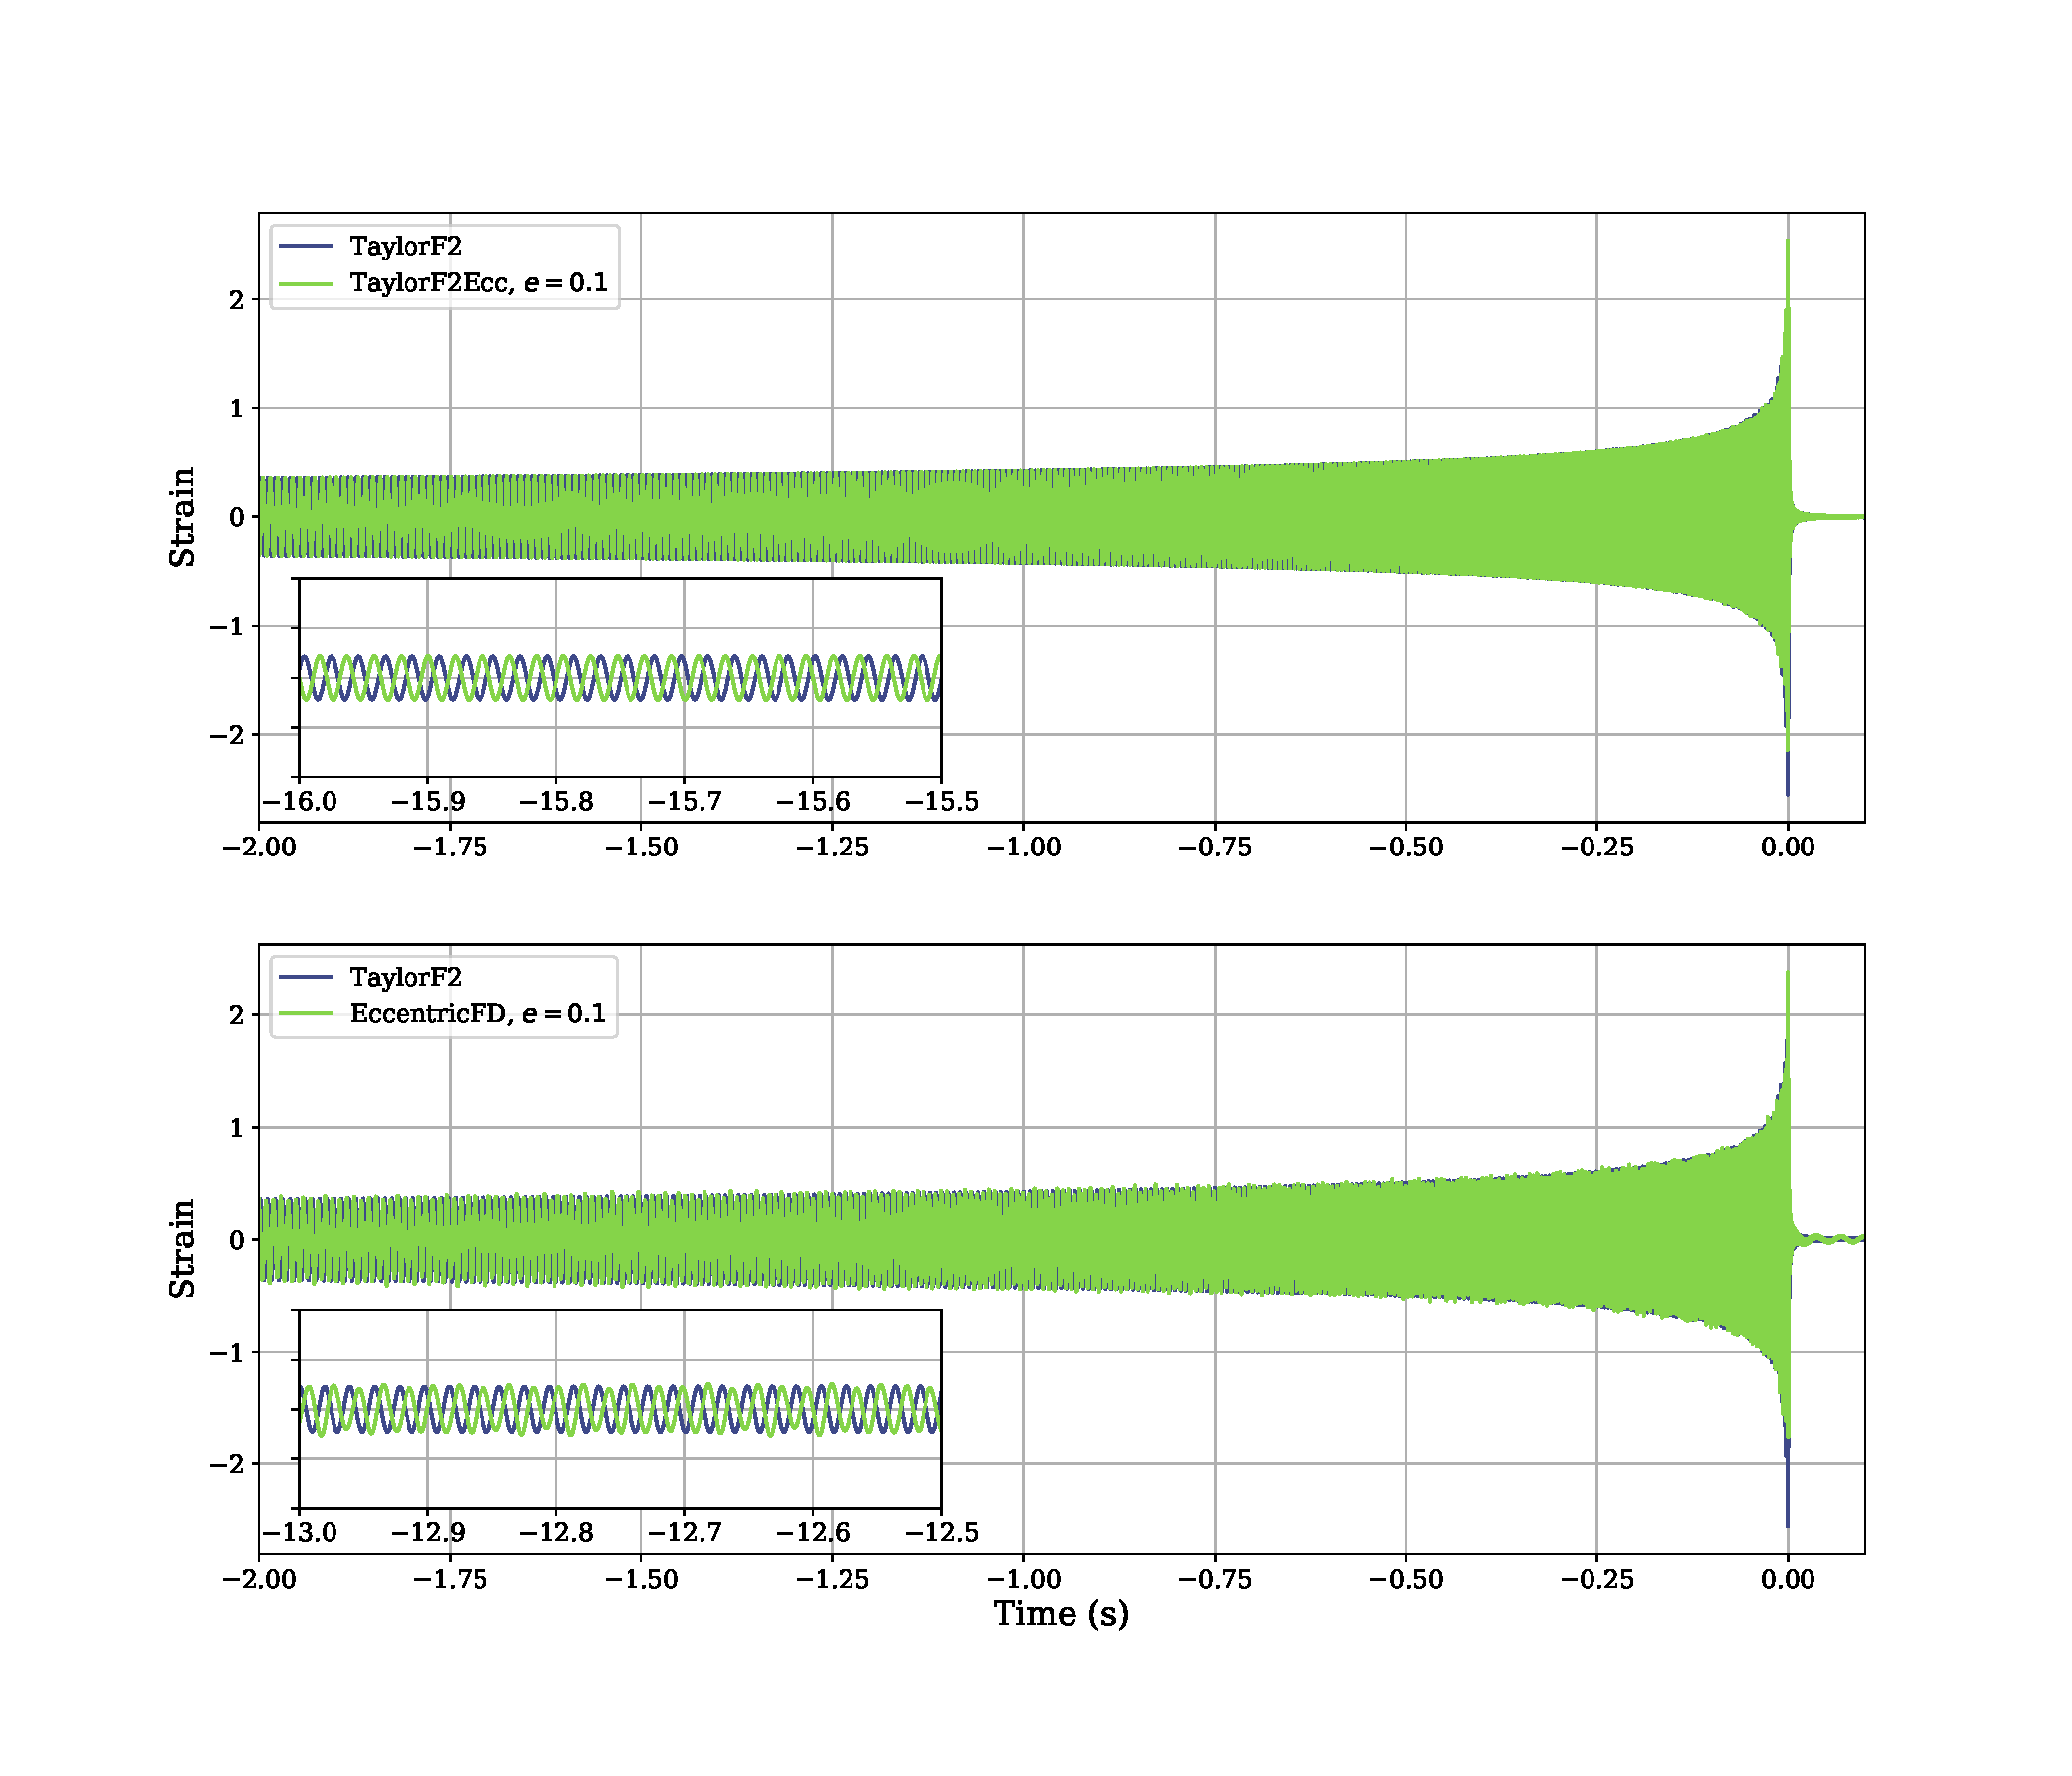
\includegraphics[width=1.0\textwidth,keepaspectratio]{Figures/Methods/Waveformplot.pdf}
    \caption{The scaled strain as a function of time for two eccentric gravitational waveform models. TaylorF2Ecc (top) EccentricFD (bottom) gravitational waveforms generated at a dominant-mode gravitational-wave reference frequency of 10Hz with component masses of 1.4$\msun$ at an eccentricity of $e=0.1$ compared with the non-eccentric TaylorF2 waveform that show merging binary neutron stars up to the time of merger. The inset plot shows a zoomed-in depiction of the the phase difference in the non-eccentric (violet) and eccentric (green) waveforms.}
    \label{fig:waveforms}
\end{figure}
\Chapter{Search for Eccentric Binary Neutron Star Mergers in the first and second observing runs of Advanced LIGO}
\label{ch:eccentric-search}
\section{Introduction}
\label{sec:intro}

\begin{figure*} 
  \centering
  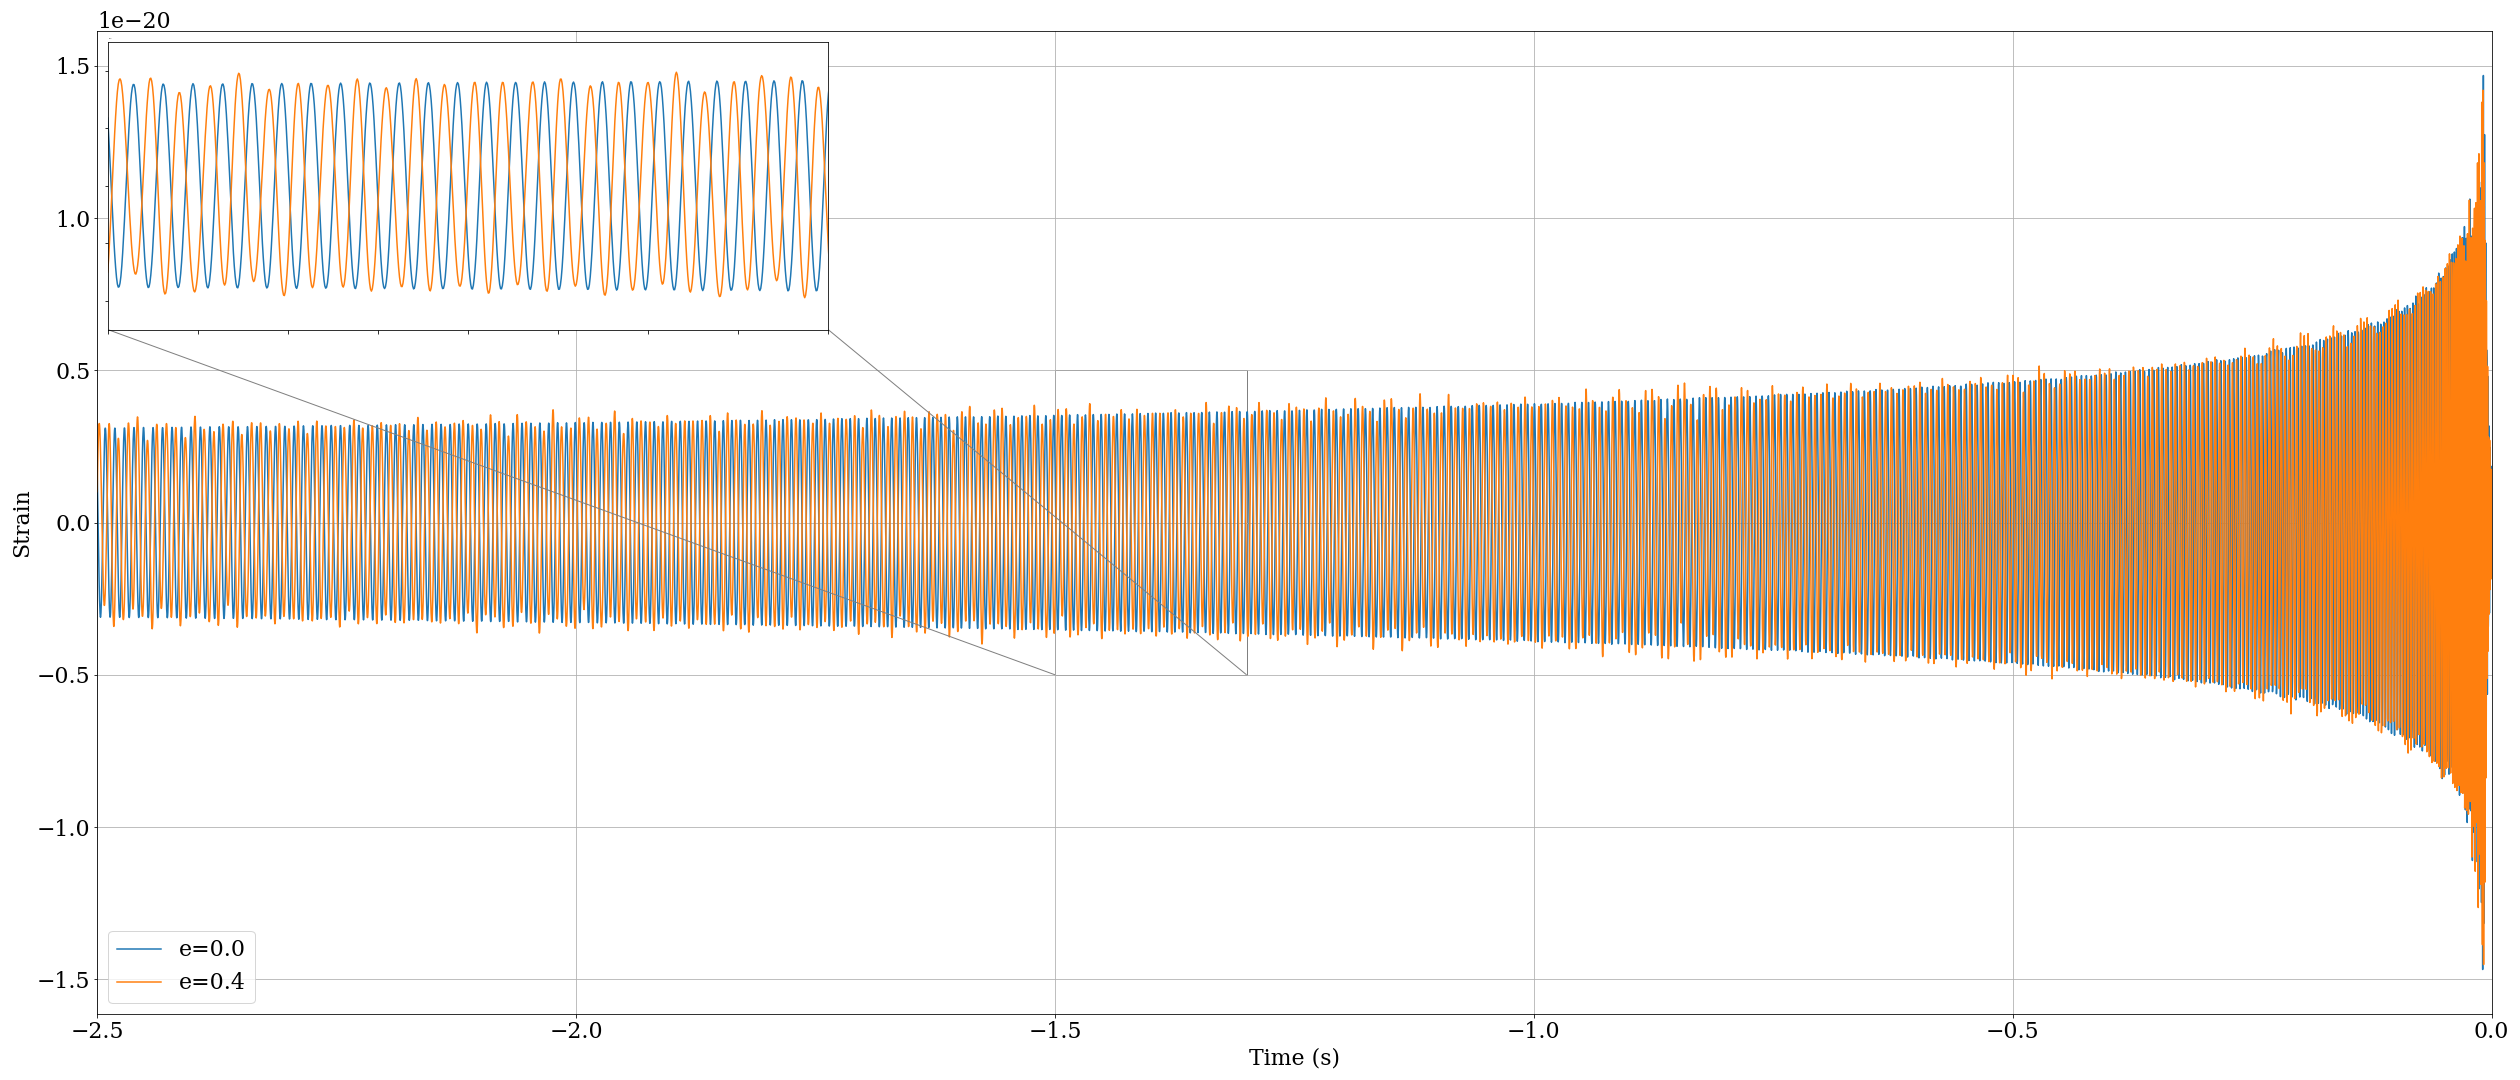
\includegraphics[width=\textwidth]{Figures/eccentric-search/tf2e_waveforms.png}
\caption{EccentricFD gravitational waveforms generated at a dominant-mode gravitational-wave reference frequency of 10Hz with component masses of 1.3$\msun$ for a non-eccentric, e=0.0, (blue) and eccentric, e=0.4, (orange) merging binary neutron star up to the time of merger. Though the waveforms look similar they overlap by $\sim 16\%$. The inset plot shows a zoomed-in depiction of the the phase difference in the non-eccentric (blue) and eccentric (orange) waveforms from -9.0 to -8.7s.}
\label{fig:waveform}
\end{figure*}

With the detections made by the Advanced LIGO (Laser Interferometer Gravitational Wave Observatory)~\cite{TheLIGOScientific:2014jea} and Virgo observatories~\cite{TheVirgo:2014hva}, we have entered the age of gravitational-wave astronomy. During their first (O1) and second (O2) observing runs, the LIGO and Virgo collaborations detected ten binary black hole (BBH) mergers and one binary neutron star (BNS) merger~\cite{LIGOScientific:2018mvr}. Independent groups have since verified these events and detected several additional binary black hole mergers~\cite{Venumadhav:2019tad,Venumadhav:2019lyq,Nitz:2018imz,Nitz:2019hdf}. One possible channel for the formation of merging binaries is through dynamical interaction in dense stellar environments such as globular clusters~\cite{Sigurdsson:1993zrm,PortegiesZwart:1999nm,Grindlay:2005ym} or galactic nuclei~\cite{Oleary:2008myb,Antonini:2012ad}. Unlike binaries formed in the field which can radiate away their eccentricity~\cite{Peters:1964,Hinder:2007qu}, dynamically formed binaries may still have significant residual eccentricity when their gravitational waves enter the LIGO-Virgo band. The observation of a binary with measurable eccentricity would confirm the existence of a dynamical formation channel. The existing LIGO-Virgo BBH candidates are consistent with non-eccentric binary mergers~\cite{Romero-Shaw:2019itr}. The third LIGO-Virgo observing run is currently underway and is expected to produce dozens more events~\cite{Aasi:2013wya}. 

A search for eccentric BBH mergers in O1 and O2 data using methods which do not use models of the gravitational waveform~\cite{Klimenko:2008fu,Klimenko:2015ypf,Tiwari:2015gal} reported no eccentric merger candidates~\cite{Salemi:2019owp}. The sensitivity of gravitational-wave searches can be improved by the use of matched-filtering, if a model of the target waveform is available. Existing matched-filter searches were designed for the detection of circular  binaries~\cite{DalCanton:2017ala,Usman:2015kfa,Venumadhav:2019tad}. It is possible that compact binaries with measurable eccentricity may have been missed by these initial searches~\cite{Brown:2009ng,Huerta:2013qb}. For BBH mergers, highly accurate models with the full inspiral-merger-ringdown, along with support for both a large range of eccentricity and spin do not yet exist, though development is rapidly progressing and there are models which satisfy some of these constraints~\cite{Huerta:2017kez,Cao:2017ndf,Hinderer:2017jcs,Hinder:2017sxy,Ireland:2019tao}.

In this paper, we search for eccentric BNS mergers.  There are several models of the gravitational waveform suitable for this task which include EccentricFD~\cite{Huerta:2014eca} and TaylorF2e~\cite{Moore:2018kvz,Moore:2019xkm}. These waveform models do not currently support compact-object spin. However, neutron star binaries formed by dynamical capture in globular clusters may have non-negligible spin if they follow the observed distribution of millisecond pulsars (MSPs). Even if large spins are supported, we may expect the  effective spin $\chieff = (\chi_{1z} m_1 + \chi_{2z} m_2)/(m_1+m_2)$ to peak around zero if the individual neutron stars orientations are isotropic. Searches which do not account for spin still have significant sensitivity to sources with low effective spin $\chieff < 0.1$, though there will be significantly reduced sensitivity in the case where both component neutron stars are consistent with the fastest observed MSP~\cite{Hessels:2006ze} and their respective spins are aligned with the orbital angular momentum~\cite{Brown:2012gs}.

Using these waveforms, we perform a matched-filtering based analysis by extending the methods used by Ref.~\cite{Nitz:2018imz} to include eccentric binaries. We find that our search is effective at detecting eccentric BNS mergers up to an eccentricity \ecc~$\sim 0.43$ at a dominant-mode gravitational-wave frequency of 10 Hz. Using a representative sample of the O1 and O2 dataset, we find that a non-eccentric search starts losing significant sensitivity relative to the eccentric search starting at $\ecc \sim 0.07$, in agreement with the results of~\cite{Huerta:2013qb,Moore:2019vjj}.

We find no individually significant eccentric BNS merger candidates using the public O1 and O2 datasets~\cite{Vallisneri:2014vxa}. The only significant event is the previously reported merger GW170817~\cite{TheLIGOScientific:2017qsa} since our search is also sensitive to circular binaries. In the absence of a new detection, we place a $90\%$ upper limit on the merger rate of $\sim 1700~\textrm{Gpc}^{-3}\textrm{Yr}^{-1}$ for binaries whose eccentricity is \ecc~$\lesssim0.43$ at the 10 Hz reference frequency. While we do not detect any individually significant mergers, it is possible that follow-up could uncover sub-threshold sources, and so we make available our full population of sub-threshold candidates~\cite{1-ECCBNS}.

We can compare our measured rate to predictions for the proposed channels for eccentric BNS formation. Ref.~\cite{Lee:2009ca} predict a BNS merger rate of 30 $\textrm{Gpc}^{-3} \textrm{Yr}^{-1}$ at z=0 from binaries formed by the tidal capture and collision of neutron stars in globular clusters. Ref.~\cite{Ye:2019xvf} predict a merger rate of $\sim 0.02 \textrm{Gpc}^{-3} \textrm{Yr}^{-1}$ from binaries formed by dynamical interactions in globular clusters. Given these predicted rates, it is unsurprising that our search did not observe a signal. Future detectors like A+~\cite{Aasi:2013wya} and Cosmic Explorer~\cite{Reitze:2019iox}, will observe a large volume of the universe and have a higher probability of observing eccentric BNS mergers. Using our measured rate and the expected sensitivity of A+ and Cosmic Explorer, we estimate the time it would take for observed rates to impinge on the predicted rates. Using the A+ expected sensitivity distance of 330 Mpc~\cite{Aasi:2013wya}, we find the most optimistic predictions~\cite{Lee:2009ca} require half a year of data for the measurement to be comparable to the predictions. The most pessimistic predictions~\cite{Ye:2019xvf}  require $\sim 775$ years of data before the measured rate limits are comparable with the prediction. However, the proposed third-generation detector Cosmic Explorer would need at most half a year of data to achieve a rate limit comparable to the most pessimistic models, although a serendipitous detection is always a possibility with  current detectors.

\section{Search Methodology}   

We use a matched-filtering search for compact-object binaries  using the PyCBC toolkit~\cite{pycbc-github}. We use gravitational waveforms that model mergers with elliptical orbits, but otherwise employ the same configuration as used by Ref.~\cite{Nitz:2018imz} for their search for gravitational waves from compact binary mergers.

\begin{figure}[t] 
  \centering
    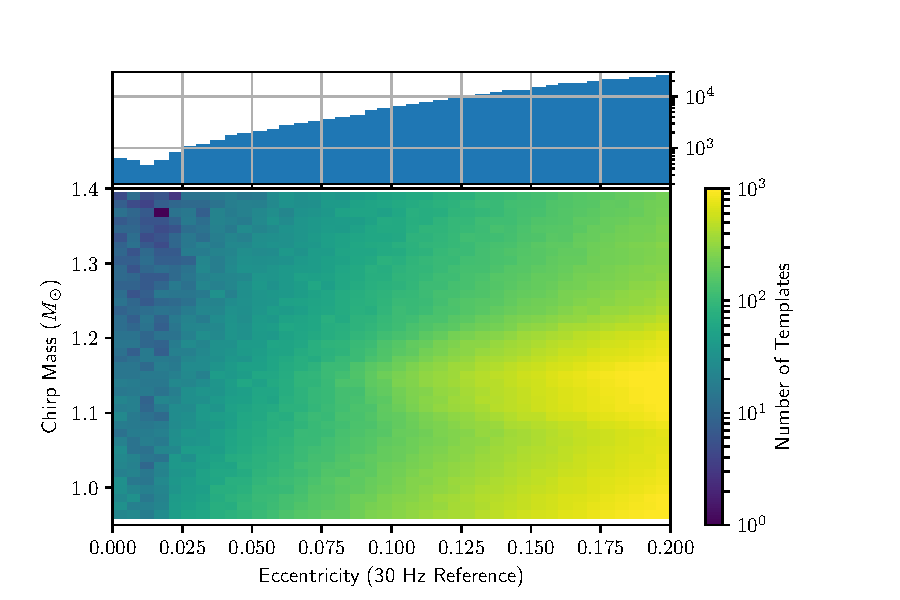
\includegraphics[width=\textwidth]{Figures/eccentric-search/bank.pdf}
\caption{This distribution of templates in our eccentric BNS bank. Note that the eccentricity
is given at a dominant-mode gravitational-wave reference frequency of 30 Hz as opposed to 10 Hz used elsewhere in this paper.}
\label{fig:bank}
\end{figure}

Of the available waveform models, we employ two waveform models that contain eccentricity, EccentricFD and TaylorF2e. EccentricFD~\cite{Huerta:2014eca} extends the post-circular (PC) analysis of \cite{Yunes:2009yz} to obtain a 3.5PN Fourier-domain enhanced PC gravitational-wave model that produces an eccentric, compact binary inspiral waveform in the small eccentricity approximation.  In the zero eccentricity limit this model reproduces the non-eccentric model, TaylorF2, and in the small eccentricity limit this model will reproduce the PC model to leading order. Figure~\ref{fig:waveform} shows two waveforms generated using EccentricFD with a non-eccentric waveform shown in blue and an eccentric waveform shown in orange. TaylorF2e is a 3PN Fourier-domain, eccentric waveform model, valid for larger initial eccentricities, defined by the stationary phase approximation (SPA) of a harmonically-decomposed time-domain signal. While both models expand the amplitude coefficients in small eccentricity, the TaylorF2e model does not invert the dependence of orbital frequency on eccentricity and numerically solves the stationary phase condition~\cite{Moore:2018kvz,Moore:2019xkm,Moore:2019vjj}.

We find that a template bank generated by straightforward stochastic placement of EccentricFD waveforms starting at a gravitational-wave frequency of 30 Hz is sufficient to recover BNS signals with eccentricity as modelled by either EccentricFD or TaylorF2e. In addition to the component masses of the BNS, our bank adds a parameter for the eccentricity, $\eccthirty$, along with an additional binary orientation parameter. Our template bank is designed to detect BNS mergers where the component masses range from $1.1-1.6 \msun$~\cite{Ozel:2016oaf} and eccentricities up to 0.2 at a reference of 30 Hz. This corresponds to $\sim0.43$ at a reference frequency of 10 Hz. Fig.~\ref{fig:bank} shows the distribution of templates in both chirp mass and eccentricity. The density of templates increases rapidly with eccentricity. Adding the additional degrees of freedom increases the size of the template bank by a factor of $160$ relative to a non-eccentric, non-spinning bank that would cover the same region. Due to the inherent degeneracy between the component masses, the template bank will have significant sensitivity outside this parameter space in regions where the chirp mass $\mathcal{M} = (m_1m_2)^{3/5} / (m_1+m_2)^{1/5}$ is otherwise consistent i.e. a $1.2 - 2.0\msun$ merger. 

Matched-filtering is used to calculate the signal-to-noise (SNR) time series using our bank of template waveforms independently for each observatory~\cite{Allen:2005fk}. Peaks in the SNR time series are followed up by a series of signal consistency tests~\cite{Nitz:2017lco,Allen:2004gu} and combined into multi-detector candidates~\cite{Usman:2015kfa,Nitz:2017svb}. We assign each candidate a ranking statistic, \rankingstat, using the same methods employed in the 1-OGC catalog~\cite{Nitz:2018imz}. The ranking statistic, \rankingstat, accounts for the signal-to-noise (SNR) of each candidate, the consistency of its morphology and signal properties with an astrophysical source, and the rate of background for candidates arising from similar templates.

\section{Observational Results}
\begin{table*}
  \begin{center}
\resizebox{\textwidth}{!}{
\begin{tabular}{ccrcrrrrrrrr}
Date designation & GPS time & FAR$^{-1}$ (y) & $\rankingstat$ & $\rho_H$ & $\rho_L$ & $m_1$ & $m_2$ & $\eccthirty$\\ \hline
170817+12:41:04UTC          & 1187008882.45          &   $>10000$                     &      27.86          &      18.41          &      23.60          &       1.48          &       1.28          &       0.02         \\
151127+02:24:56UTC          & 1132626313.67          &        .57                     &       8.60          &       7.28          &       5.73          &       1.23          &       1.55          &       0.16         \\
151130+22:40:53UTC          & 1132958470.76          &        .54                     &       8.60          &       6.76          &       5.89          &       1.29          &       1.22          &       0.19         \\
170705+12:02:50UTC          & 1183291388.00          &        .31                     &       8.54          &       7.29          &       5.56          &       1.48          &       1.57          &       0.16         \\
151227+13:12:35UTC          & 1135257172.28          &        .14                     &       8.42          &       6.33          &       6.21          &       1.42          &       1.37          &       0.10         \\
170618+15:35:01UTC          & 1181835319.00          &        .08                     &       8.40          &       7.30          &       5.35          &       1.22          &       1.19          &       0.15         \\
170812+20:07:43UTC          & 1186603681.67          &        .07                     &       8.35          &       6.92          &       5.47          &       1.21          &       1.13          &       0.17         \\
170302+22:45:10UTC          & 1172529928.62          &        .07                     &       8.42          &       6.93          &       5.46          &       1.23          &       1.17          &       0.12         \\
161222+07:49:11UTC          & 1166428168.98          &        .06                     &       8.39          &       6.33          &       6.14          &       1.50          &       1.12          &       0.18         \\
170328+07:26:40UTC          & 1174721218.74          &        .05                     &       8.38          &       5.11          &       7.26          &       1.11          &       1.22          &       0.12         \\
\end{tabular}}
    \caption{Binary neutron star candidates from the search of O1 and O2 LIGO data sorted by the rate of false alarms with a detection statistic at least as large as the candidate. The mass and eccentricity parameters of the template associated with each candidate are listed. Note the eccentricity is given at the 30 Hz gravitational-wave frequency reference used to generate the template bank. The values associated with a candidate can be considered point estimates and may differ significantly from the results of full Bayesian parameter estimation. Masses are quoted in the detector frame.}
    \label{table:search}
  \end{center}
\end{table*}


We search the public LIGO O1 and O2 dataset which contains $\sim164$ days of coincident LIGO-Hanford and LIGO-Livingston data after removal of data which has been flagged as potentially containing instrumental artefacts~\cite{TheLIGOScientific:2016zmo,TheLIGOScientific:2017lwt,Vallisneri:2014vxa}. Data when only a single observatory was operating was not considered, nor was data from the Virgo observatory which operated only in the last month of O2. In this search, we neglect data from the Virgo detector as it only provides a marginal senstivity improvement~\cite{Nitz:2019hdf}. Future analyses will incorporate data from the full network.

The most significant candidates are listed in Table~\ref{table:search}. As our search is also sensitive to circular binaries, it is not surprising that GW170817---first detected by the LIGO-Virgo search for circular binaries---was observed as a high-significance event. The remaining candidates are consistent with the rate of false alarms expected for the amount of data analyzed. However, we cannot rule out a sub-threshold population which may be uncovered by correlation with non-GW datasets (GRBs, Kilonovae, etc) such as performed in Ref.~\cite{Nitz:2019bxt}.

\section{Upper Limits}

\begin{figure}[t]
  \centering
    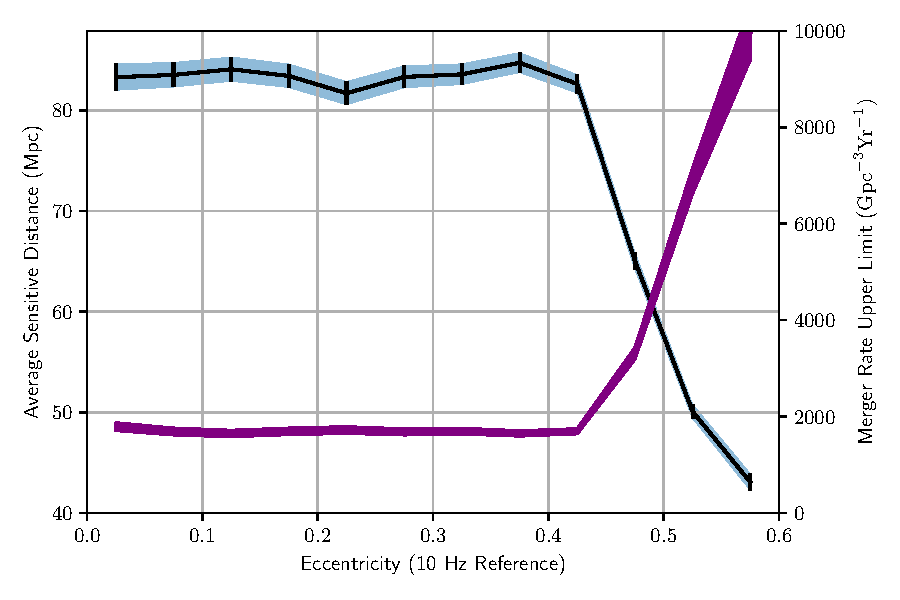
\includegraphics[width=\textwidth]{Figures/eccentric-search/rate.pdf}
\caption{The average sensitive distance of the search (blue/left scale) and the 90$\%$ upper limit on the rate of eccentric binary neutron star mergers (purple/right scale) as a function of eccentricity at a reference frequency of 10 Hz. The average sensitivity is nearly flat up to an eccentricity of 0.43, where we begin to see sharp drop-off in sensitive range. This corresponds to the edge of our template bank.
}
\label{fig:range}
\end{figure}

As our search did detect any significant individual eccentric BNS merger candidates, we place an upper limit on the rate of eccentric mergers as a function of their eccentricity. We determined a $90\%$ confidence upper limit on the rate of mergers using the method introduced in Ref.~\cite{Brady:2004gt}. The upper limit on the merger rate $R_{90}$ is

\begin{equation}
    R_{90} = 2.303 \left[TV(\mathcal{F}^*)\right]^{-1}
\end{equation}

where $T$ is the total observation time and $V(\mathcal{F^*})$ is the average volume the search is sensitive to at the false alarm rate of the loudest observed candidate. Under the assumption that GW170817 is a non-eccentric merger, we exclude it from our analysis. The sensitivity is measured using a simulated population of sources distributed uniform in volume and isotropic in orientation. We have primarily used the EccentricFD model for our simulated population, however, we have confirmed our results are consistent with a smaller sample using the TaylorF2e model. Fig.~\ref{fig:range} shows the upper limit on the merger rate as a function of the binary eccentricity as well as the average sensitive distance of the search over the observation period. We find that up to an eccentricity of $\sim 0.43$ at a reference frequency of 10 Hz, we can place a $90\%$ upper limit at $\sim$1700 mergers per cubic Gpc per year.

Under the assumption that eccentric signals will not have been detected, we can determine the observation time required by future detectors to constrain the BNS merger rates predicted by Ref.~\cite{Lee:2009ca} and Ref.~\cite{Ye:2019xvf} by scaling the upper limit from our search. We find that the Advanced LIGO observatories had an average range, $D_{O1+O2}$, of 90 Mpc during O1 and O2 for a fiducial $1.4-1.4 \msun$ merger by taking the weighted-average of their noise curves. Similarly, using their respective noise curves, we find an average range, $D_{A+}$, of 330 Mpc for A+~\cite{Aasi:2013wya} and $D_{CE}$ of 7130 Mpc for Cosmic Explorer\footnote{https://cosmicexplorer.org/researchers.html}. The observation time required, $T_{CE,A+}$, to match the predicted rates, $R_{Ye, Lee}$, is given as
\begin{equation}
    T_{CE,A+|Ye,Lee} = T_{O1+O2} \frac{R_{O1+O2}}{R_{Ye,Lee}} \left(\frac{D_{O1+O2}}{ D_{CE,A+}}\right)^3,
\end{equation}
where $T_{O1+O2}$ is the total observation time of O1 and O2 and $R_{O1+O2}$ is the upper limit achieved by our current search. We find that with the increased sensitivity of A+ the most optimistic predictions~\cite{Lee:2009ca} would require half a year of data and the most pessimistic predictions~\cite{Ye:2019xvf} would require $\sim 775$ years. Cosmic Explorer would need at most half a year of data to constrain current BNS merger rate models. Understanding the constraints that future observational limits place on eccentric binary formation channels will require computation of the rate as a function of eccentricity from population synthesis.

\section{Conclusions}

We have developed a search that is effective at detecting BNS mergers with orbital eccentricity $\lesssim0.43$ at 10 Hz. Our search uses the public PyCBC toolkit~\cite{pycbc-github} based on a standard matched filtering approach~\cite{Nitz:2018imz,Usman:2015kfa}. We have found that straightforward stochastic placement algorithms are sufficient to tackle the construction of template banks for eccentric binary merger waveforms. As broadly applicable and highly accurate eccentric waveform models are developed which include corrections for component-object spin, the full inspiral-merger-ringdown, and support for large values of eccentricity it will be possible to apply the same methods demonstrated here to the detection of BBH mergers.

To aid in further analysis of our results, we make available our full sub-threshold catalog of eccentric BNS candidates. For each candidate we provide the false alarm rate, parameters of the associated template waveform, and signal parameters such as the signal-to-noise and results of our signal consistency tests~\cite{1-ECCBNS}\footnote{\texttt{\url{www.github.com/gwastro/eccentric-bns-search}}}.

While the detection of a single BNS or BBH eccentric merger would immediately demonstrate the existence of dynamical formation, current estimates of the rate of BNS mergers imply that a single observation would be rare for the current generation of ground based observatories. Future observatories such as Cosmic Explorer will be able to probe current models.

\label{sec:disc}

\Chapter{Measuring the Eccentricity of GW170817 and GW190425}
\label{ch:bns-pe}
Two binary neutron star mergers, GW170817 and GW190425, have been detected by Advanced LIGO and Virgo. These signals were detected by matched-filter searches that assume the star's orbit has circularized by the time their gravitational-wave emission is observable. This suggests that their eccentricity is low, but full parameter estimation of their eccentricity has not yet been performed. We use gravitational-wave observations to measure the eccentricity of GW170817 and GW190425. We find that the eccentricity at a gravitational-wave frequency of 10 Hz is  $e \leq 0.024$ and $e \leq 0.048$ for GW170817 and GW190425, respectively (90\% confidence). This is consistent with the binaries being formed in the field, as such systems are expected to have circularized to $e \leq 10^{-4}$ by the time they reach the LIGO-Virgo band. Our constraint is a factor of two smaller that an estimate based on GW170817 being detected by searches that neglect eccentricity. However, we caution that we find significant prior dependence in our limits, suggesting that there is limited information in the signals. We note that other techniques used to constrain binary neutron star eccentricity without full parameter estimation may miss degeneracies in the waveform, and that for future signals it will be important to perform full parameter estimation with accurate waveform templates.

\section{Introduction}
\label{sec:pe-intro}
The Advanced LIGO and Virgo observatories have detected two binary neutron star mergers, GW170817 \cite{TheLIGOScientific:2017qsa} and GW190425 \cite{Abbott:2020uma}. To date, 17 double neutron star systems have been observed through radio surveys of the Milky Way field \cite{Martinez:2017jbp,Tauris:2017omb,Cameron:2017ody,Stovall:2018ouw,Lynch:2018zxo}. Observations of binary neutron stars allow us to determine their formation channels \cite{Smarr1976,Canal:1990dz,PortegiesZwart1:1997zn,Postnov:2006hka,Kalogera:2006uj,Kowalska:2010qg,Tauris:2017omb,Belczynski:2018ptv,Vigna-Gomez:2018dza,Giacobbo:2018etu,Mapelli:2018wys,Andrews:2019vou}, constrain the neutron-matter equation of state \cite{Bauswein:2017vtn,Annala:2017llu,Fattoyev:2017jql,De:2018uhw,Abbott:2018exr,Capano:2019eae,Tews:2018iwm,Most:2018hfd,Radice:2018ozg,Coughlin:2018fis,Forbes:2019xaz}, and test the strong-field regime of general relativity \cite{Abbott:2018lct}.

Although the eccentricity of double neutron stars in the Milky Way field ranges from $0.06$ to $0.828$ \cite{Zhu:2017znf,Andrews:2019vou}, field binaries will circularize to eccentricity $e \leq 10^{-4}$ \cite{Peters:1964zz,Kowalska:2010qg}, making them detectable by matched-filter searches that neglect eccentricity \cite{Martel:1999tm,Cokelaer:2009hj,Brown:2009ng,Huerta:2013qb}.
GW170817 and GW190425 were detected by searches that neglect eccentricity \cite{TheLIGOScientific:2017qsa,Abbott:2020uma}, suggesting that their eccentricity is $e \lesssim 0.05$ \cite{Huerta:2013qb}, however no direct measurement of their eccentricity has been made. Ref.~\cite{Romero-Shaw:2020aaj} place a limit on the eccentricity of GW190425 by estimating the effect of eccentricity on the measured parameters of the signal. Here, we directly measure the eccentricity of GW170817 and GW190425 using Bayesian parameter estimation \cite{Biwer:2018osg}.

We use the observations from the Gravitational-Wave Open Science Center \cite{TheLIGOScientific:2017qsa,Abbott:2020uma}, waveform templates that include eccentricity \cite{Moore:2016qxz}, and Markov Chain Monte Carlo parameter estimation \cite{ForemanMackey:2012ig,Biwer:2018osg} to measure the eccentricity of the GW170817 and GW190425 when they have a gravitational-wave frequency of 10 Hz. We find that the eccentricity of GW170817 is $e \leq 0.027$ and GW190425 is $e \leq 0.052$ at 90\% confidence for a uniform prior on $e$. Our limit on eccentricity of GW170817 is a factor of two smaller than the limit estimated by its detection with circular waveform templates. We note that when using a common prior on eccentricity, our limit on the eccentricity of GW190425 is a factor of three greater than the limit of Ref.~\cite{Romero-Shaw:2020aaj}. We find that this is due to a degeneracy between the chirp mass and eccentricity that is not included in the analysis of Ref.~\cite{Romero-Shaw:2020aaj}. However, this difference does not invalidate their conclusions about the formation of GW190425.

Dynamical interations may form binary neutron stars with residual eccentricity, although the rate of such mergers is expected to be small in current detectors \cite{Lee:2009ca,Ye:2019xvf} and a search for eccentric binary neutron stars in the O1 and O2 observing runs did not yield any candidates \cite{Nitz:2019spj}. However, since eccentricity is an interesting probe of binary formation channels and eccentric binaries may produce different electromagnetic emission than circular binary neutron stars \cite{Radice:2016dwd,Chaurasia:2018zhg}, it is important to accurately constrain the eccentricity of binary neutron stars as the number of observed mergers increases in the coming years.

\section{Methods}

\label{sec:pe-method}

We measure the parameters of GW170817 and GW190425 using Bayseian inference \cite{Finn:2000hj,Rover:2006ni}. We use gravitational-wave data from Advanced LIGO and Virgo \cite{Blackburn:170817,dataLIGO:190425}, $\boldsymbol{d}(t)$, and a model of the gravitational waves, $H$, to calculate the posterior probability density function, $p(\boldsymbol{\theta}|\boldsymbol{d}(t),H)$, given by
\begin{equation}
    p(\boldsymbol{\theta}|\boldsymbol{d}(t),H) = \frac{p(\boldsymbol{\theta}|H) p(\boldsymbol{d}(t)|\boldsymbol{\theta},H)}{p(\boldsymbol{d}(t)|H)},
\end{equation}
where $\boldsymbol{\theta}$ denotes the parameters of the gravitational waveform, $p(\boldsymbol{\theta}|H)$, is the prior distribution on the signal parameters, and $p(\boldsymbol{d}(t)|\boldsymbol{\theta},H)$, is the probability of observing the data, known as the likelihood. The likelihood models the noise in the detector as a Gaussian and depends upon a noise-weighted inner product between the gravitational waveform and gravitational-wave data, $\boldsymbol{d}(t)$. Markov Chain Monte Carlo (MCMC) techniques can be used to marginalize over the parameters to obtain the posterior probabilities \cite{Christensen:2001cr}. Our implementation of Bayesian inferences uses the \textit{PyCBC Inference} software package \cite{Biwer:2018osg,alex_nitz_2020_3630601} and the parallel-tempered \textit{emcee} sampler, \texttt{emcee\_pt} \cite{ForemanMackey:2012ig,emceept}.

For GW170817 and GW190425, the MCMC is performed over the component masses of the binary, $m_{1,2}$, the component spins aligned with the orbital angular momentum, $\chi_{1,2}$, the time of coalescence, $t_c$, the polarization of the GW, $\psi$, the inclination angle, $\iota$, and the eccentricity, $\ecc$.

We assume a uniform prior distribution on the component masses, component spins, and coalescence time around the trigger shown in Table~\ref{tab:prior}. We assume an isotropic sky location for GW190425 and a prior uniform in $\sin \iota$ for the inclination angle of both detections. We fix the sky location of GW170817 to the observed EM counterpart using a Gaussian prior distribution on the distance \cite{Cantiello:2018ffy}. We explore the prior distribution on the eccentricity by running the MCMC with two prior distributions: a prior that is uniform in $\ecc$ and a prior uniform in $\log e$ to compare with the GW190425 results found by Ref.~\cite{Romero-Shaw:2020aaj}.

We use the GW strain data from the Advanced LIGO and Virgo detectors for GW170817 and GW190425, available through the LIGO Open Science Center (LOSC) \cite{Vallisneri:2014vxa}. The \texttt{LOSC\_CLN\_4\_V1} data that we use for GW170817 includes post-processing noise-subtraction performed by the LIGO/Virgo Collaboration \cite{Blackburn:170817,Driggers:2018gii}. The \texttt{T1700406\_v3} data that we use for GW190425 includes pre-processing glitch removal performed by the LIGO/Virgo Collaboration specifically for use in parameter estimation \cite{Abbott:2020uma,dataLIGO:190425}.

We high-pass the data using an eighth-order Butterworth filter with an attenuation of 0.1 at 15 Hz. To conserve the phase of the delay, the filter is applied forward and backwards. A low-pass finite impulse response filter is applied to the data prior to resampling. The data is decimated to 2048 Hz for the analysis. For computing the likelihood, we use Welch's method to estimate the detector's noise power spectral density (PSD). Welch's method is used with 16 second Hanning windowed segments that are overlapped by 8 seconds. The PSD is shortened to 8 seconds in the time domain \cite{Allen:2005fk}. The gravitational-wave data, $\boldsymbol{d}(t)$, used in the likelihood is taken from the intervals shown in Table~\ref{tab:prior}. The gravitational-wave likelihood is evaluated from a low-frequency cutoff of 20 Hz to the Nyquist Frequency of 1024 Hz.

A variety of waveforms are available that model eccentricity \cite{Huerta:2014eca,Tanay:2016zog,Moore:2016qxz,Huerta:2016rwp,Cao:2017ndf,Hinder:2017sxy,Tiwari:2019jtz,Moore:2019xkm}. From what we know of binary neutron star mergers, we expect them to have low mass, spin, and eccentricity making TaylorF2Ecc a suitable waveform. The waveform model, H, is TaylorF2Ecc, a TaylorF2 post-Newtonian (pN) model with eccentric corrections. We use the LIGO Algorithm Library implementation \cite{lalsuite} accurate to 3.5 pN order in orbital phase \cite{Buonanno:2009zt}, 3.5 pN order in the spin-orbit interactions \cite{Bohe:2013cla}, 2.0 pN order in spin-spin, quadrupole-monopole, and self-interactions of individual spins \cite{Mikoczi:2005dn,Arun:2008kb}, and 3.0 pN order in eccentricity \cite{Moore:2016qxz}. Since TaylorF2Ecc follows TaylorF2 in its construction, the waveform will terminate at twice the orbital frequency of a particle at the innermost stable circular orbit of a Schwarzschild black hole.

As a check on our analysis, we estimate the parameters of GW170817 and GW190425 using two available waveforms: the TaylorF2Ecc waveform at $e=0$ and the TaylorF2 waveform. Our analyses are consistent with each other and with the parameters estimated by Advanced LIGO and Virgo \cite{TheLIGOScientific:2017qsa,Abbott:2020uma}. 

\section{Results}
\label{sec:pe-Results}
We first constrain the level of the eccentricity by using the TaylorF2Ecc waveform and a prior uniform in $\ecc$. We find that the 90\% credible intervals at 10 Hz for GW170817 and GW190425 are $e = 0.013^{+0.014}_{-0.011}$ and $e = 0.028^{+0.024}_{-0.024}$ respectively. A degeneracy between the chirp mass, $\chirpm$, and eccentricity, $\ecc$ and a small correlation between the effective spin, $\chieff$, and $\ecc$ are shown in our posterior distributions in Figure~\ref{Fig:GW170817} and Figure~\ref{Fig:GW190425}. Since $\chirpm$ and $\chieff$ are correlated \cite{Baird:2012cu,Safarzadeh:2020mlb}, this will create a small correlation between $\ecc$ and $\chieff$.

Ref.~\cite{Romero-Shaw:2020aaj} estimated the eccentricity of GW190425 to determine if the formation channel was due to unstable BB mass transfer. They estimate the eccentricity induced by the supernova kick in this formation scenario to be between $10^{-6}$ and $10^{-3}$ at 10 Hz. To find the eccentricity of GW190425, Ref.~\cite{Romero-Shaw:2020aaj} reweight the posterior samples from the parameter estimation performed using circular binaries to estimate the limit of the eccentricity using the same method used to estimate the eccentricity of binary black holes \cite{Romero-Shaw:2019itr}. They estimate the eccentricity of GW190425 at 10 Hz to be $e \leq 0.007$ (90\% confidence) using a prior uniform in $\log e$. They find no evidence for or against unstable BB mass transfer as their analysis is not able to distinguish the small residual eccentricity expected from the investigated formation channel. 

To more directly compare our limit on GW190425's eccentricity, we repeat our analysis using a $\log e$ prior. In Figure~\ref{Fig:1DMarginal} we can see the differences in the posterior distributions of each prior. With the $\log e$ prior we estimate the eccentricity at 10 Hz to be $e \leq 0.04$. This is a factor of three larger than interval estimated by Ref.~\cite{Romero-Shaw:2020aaj}. By re-weighting the posterior samples rather than a full MCMC, the degeneracy between $\chirpm$ and $\ecc$ is missed. We find that by excluding posterior samples with lower values of $\chirpm$, we can recover the upper limit reported by Ref.~\cite{Romero-Shaw:2020aaj}. Although our limit on the eccentricity is larger than that of Ref.~\cite{Romero-Shaw:2020aaj}, our result does not change their conclusion: indeed the strong dependence of the eccentricity posterior on the prior seen in Figure~\ref{Fig:1DMarginal} agrees with their conclusion that the signal-to-noise ratio of GW190425 is not large enough to explore the eccentricities expected in BB mass transfer. We would need to be able to determine the eccentricity at lower frequencies to distinguish the formation channel.

\section{Conclusion}
Our analysis used the gravitational-wave observations as well as a prior on the eccentricity to constrain the eccentricity of GW170817 and GW190425. Our 90\% confidence limit using a uniform prior on $\ecc$ for GW170817, $e \leq 0.027$, and GW190425, $e \leq 0.052$, are consistent with expectations since they were found by a circular search \cite{Peters:1964zz}. We have constrained the eccentricity to a factor of two smaller than estimates obtained from circular searches \cite{Brown:2009ng,Huerta:2013qb}. Our 90\% credible intervals on the eccentricity of GW190425 are a approximately a factor of six larger than the interval estimated by \cite{Romero-Shaw:2020aaj}, which used a prior uniform in $\log e$. This demonstrates the impact of prior choice, and the importance of measuring the eccentricity of signals using full parameter estimation to account for the correlation between parameters.

Unfortunately, based on current merger rate estimates the detection of an eccentric binary neutron star merger will be difficult with current observatories \cite{Lee:2009ca,Ye:2019xvf,Nitz:2019spj}, but gravitational-wave capture binaries that have $e \geq 0.8$ and could form in the LIGO-Virgo band \cite{Rodriguez:2018pss,Takatsy:2018euo}. However, since the eccentricity of the detections is expected to be low and negligible, $e \leq 0.02$, a circular search is effective in detecting them \cite{Brown:2009ng,Huerta:2013qb}. 

Current waveform models are effective for detection as spin and eccentricity are assumed to be low, but that might not be the case for future gravitational-wave signals. Future signals may have high eccentricity and spin and will need further corrections to be able to detect them efficiently and produce unbiased parameter estimates. Waveforms that better model eccentric signals will need to be developed before we are able to make a detection of a merger with a high eccentricity or spin. The detection of a binary neutron star mergers with high eccentricity or spin in future observing runs and with third generation detectors will reveal more about the formation channel of eccentric binaries and the existence of a dynamical formation channel. 

\begin{sidewaystable}
\begin{center}
\resizebox{\textwidth}{!}{
    \begin{tabular}{ccc}
        \textbf{Parameters}              & \textbf{GW170817}                 & \textbf{GW190425}                     \\  \hline
        \textbf{Component Masses} (\msun)  & {[}1.0,3.0{]}                     & {[}1.0,3.0{]}                         \\ 
        \textbf{Component Spins}         & {[}-0.05,0.05{]}                  & {[}-0.05,0.05{]}                      \\ 
        \textbf{Coalescence Time} (s)    & {[}1187008882.33,1187008882.53{]} & {[}1240215502.917,1240215503.117{]}   \\ 
        \textbf{Polarization}            & {[}0,2$\pi${]}                    & {[}0,2$\pi${]}                        \\ 
        \textbf{Inclination Angle}       & $\sin \iota$                      &  $\sin \iota$                         \\ 
        \textbf{Distance} (Mpc)          & 40.7 $\pm$ 2.36~\cite{Cantiello:2018ffy} & uniform in comoving volume                     \\ 
        \textbf{RA/Dec} ($^{\circ}$)        & 3.44615914, -0.40808407~\cite{Coulter:2017wya,Soares-Santos:2017lru} & {[}$-\pi/2$,$\pi/2${]}           \\ 
        \textbf{Eccentricity}            & {[}0.0,0.1{]}                     & {[}0.0,0.1{]}                        \\ \hline 
        \hline
        \textbf{PSD Estimation Interval} (s) & {[}1187008382,1187008918{]}   & {[}1240215003,1240215543{]}          \\
        \textbf{Likelihood Interval} (s) & {[}1187008692,1187008892{]}       & {[}1240215313,1240215513{]}          \\ 
    \end{tabular}}
\caption{Prior distributions and GPS time intervals for GW170817 and GW190425.}
\label{tab:prior}
\end{center}
\end{sidewaystable}

\begin{figure}[p]
    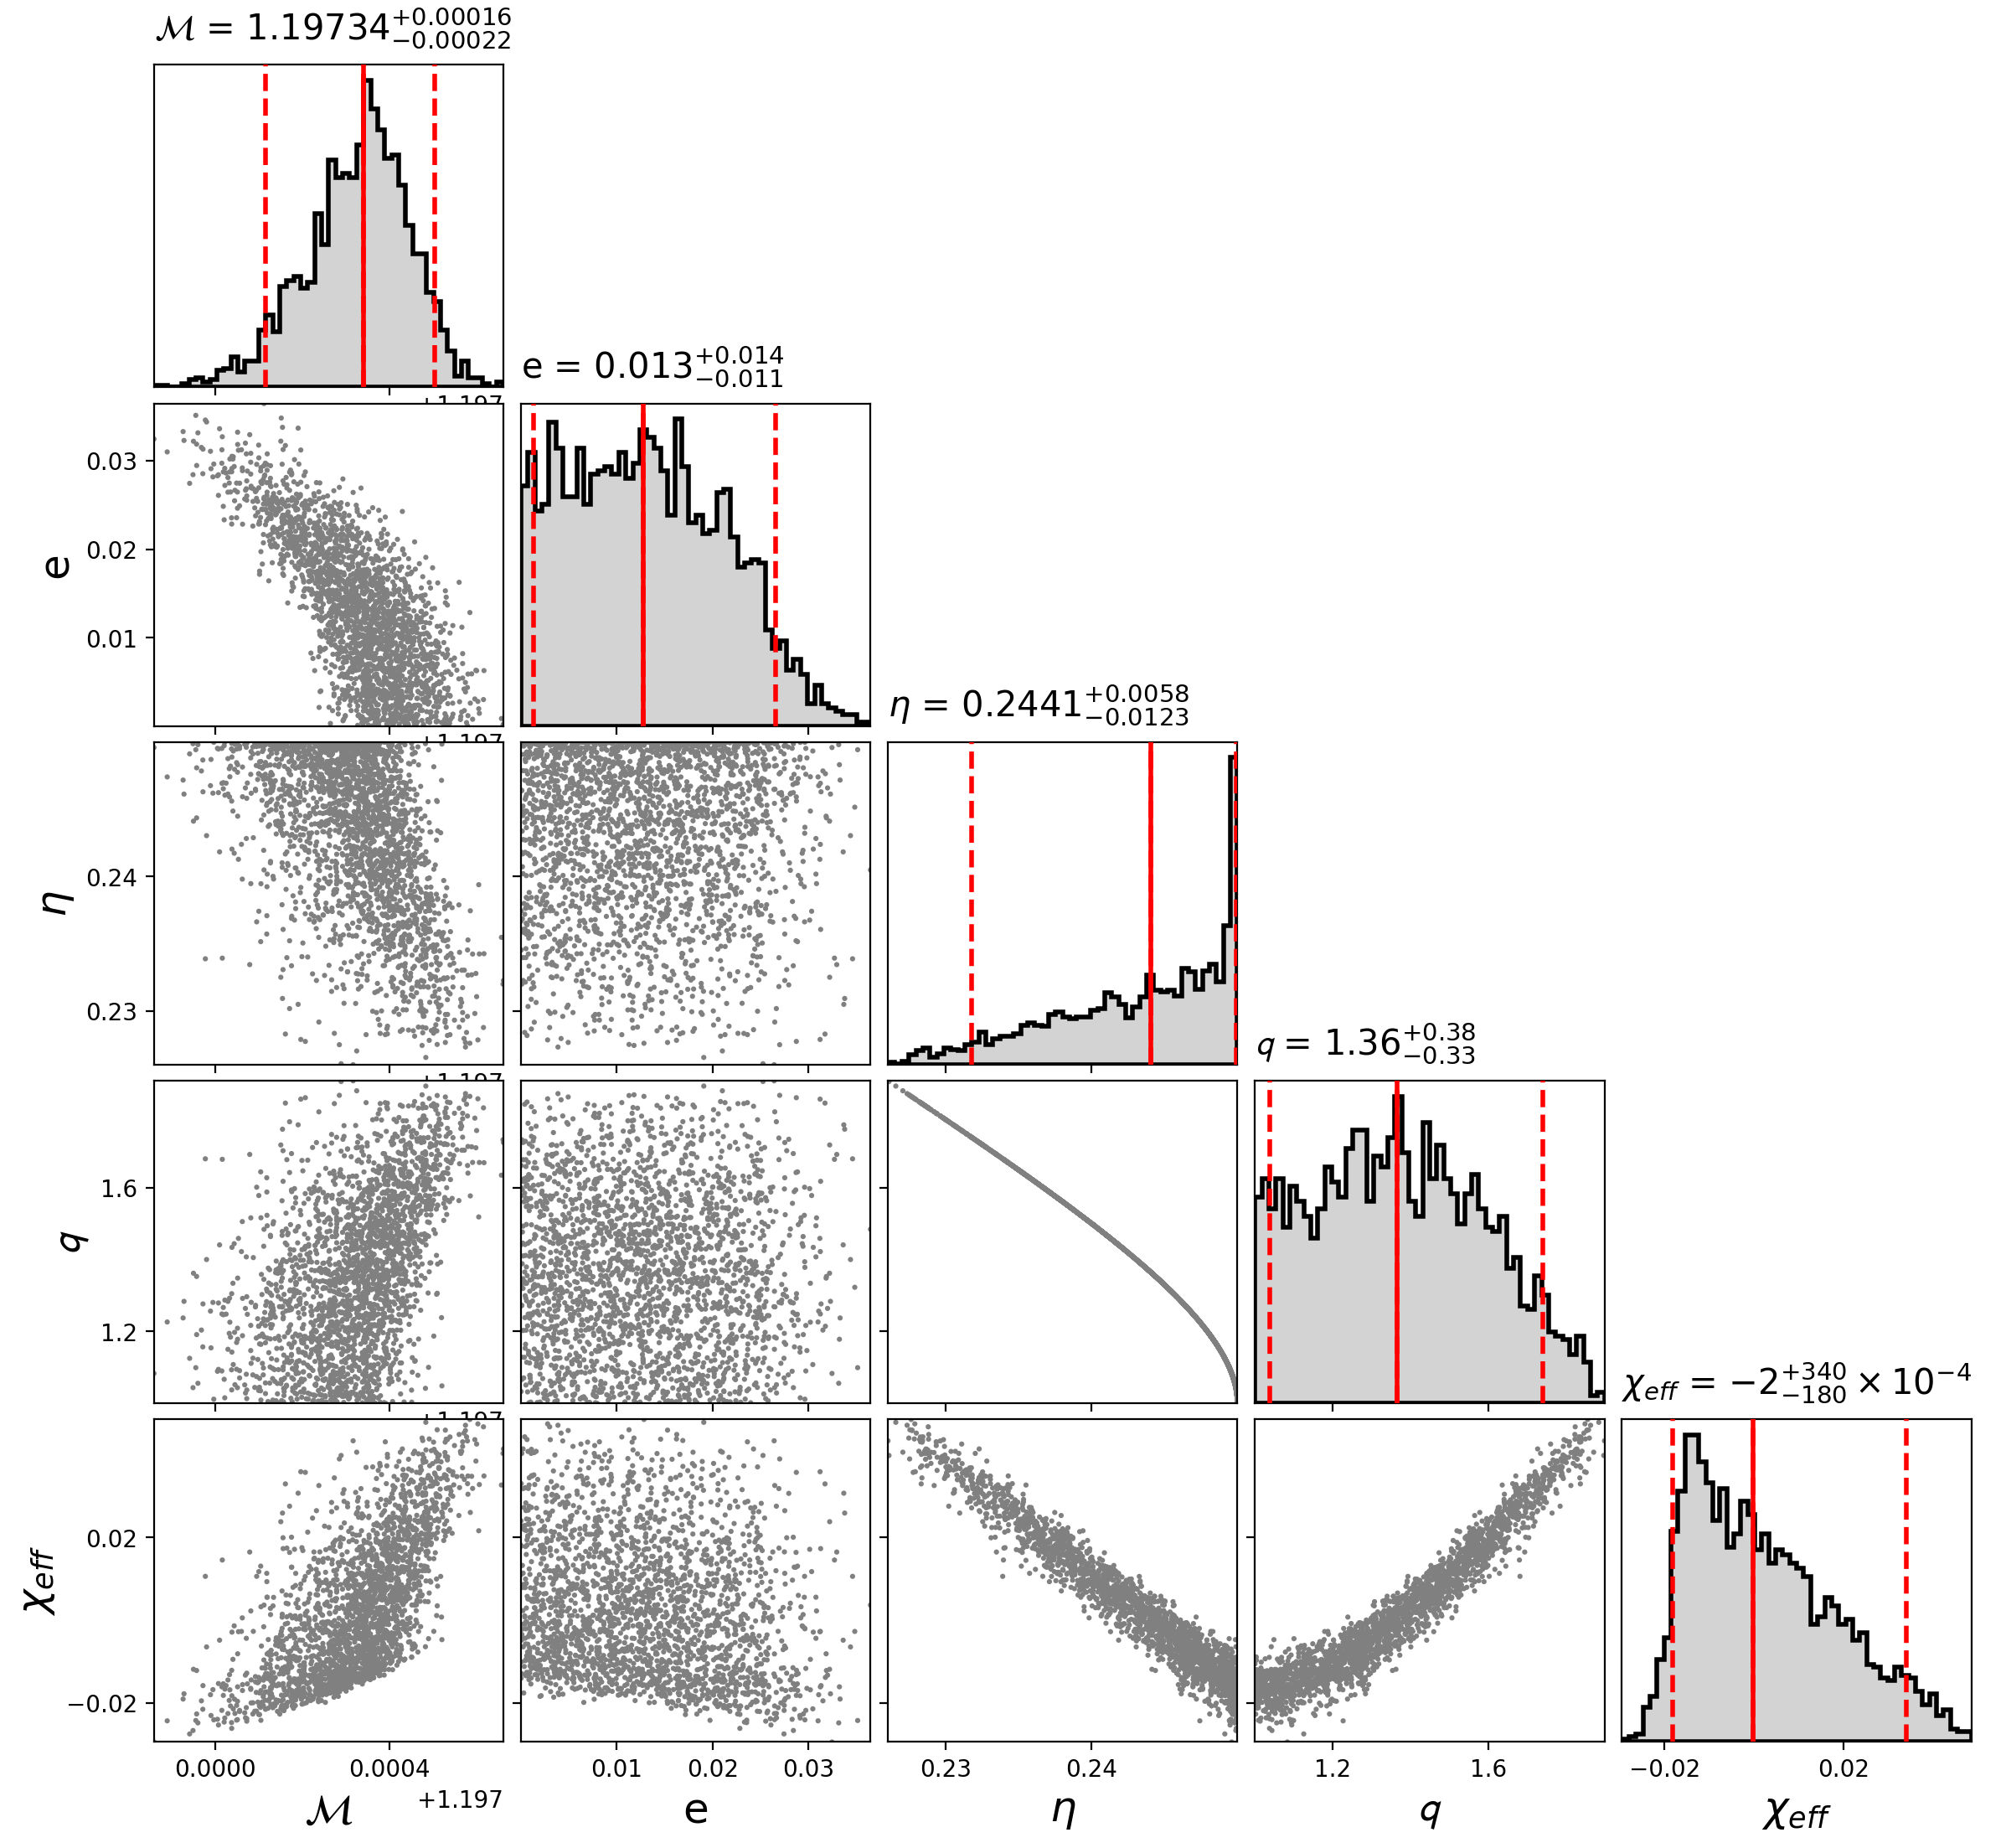
\includegraphics[width=\textwidth]{Figures/bns-pe/GW170817-e10.png}
    \caption{Posterior probability distribution of GW170817 at 10 Hz. The analysis used a prior uniform in $\ecc$. Each parameter is quoted with a median value (solid red line) and a 90\% credible interval (dashed red lines). The chirp mass $\chirpm$ is given in the detector frame. Note the degeneracy between $\chirpm$ and $\ecc$.}
\label{Fig:GW170817}
\end{figure}

\begin{figure}[p]
    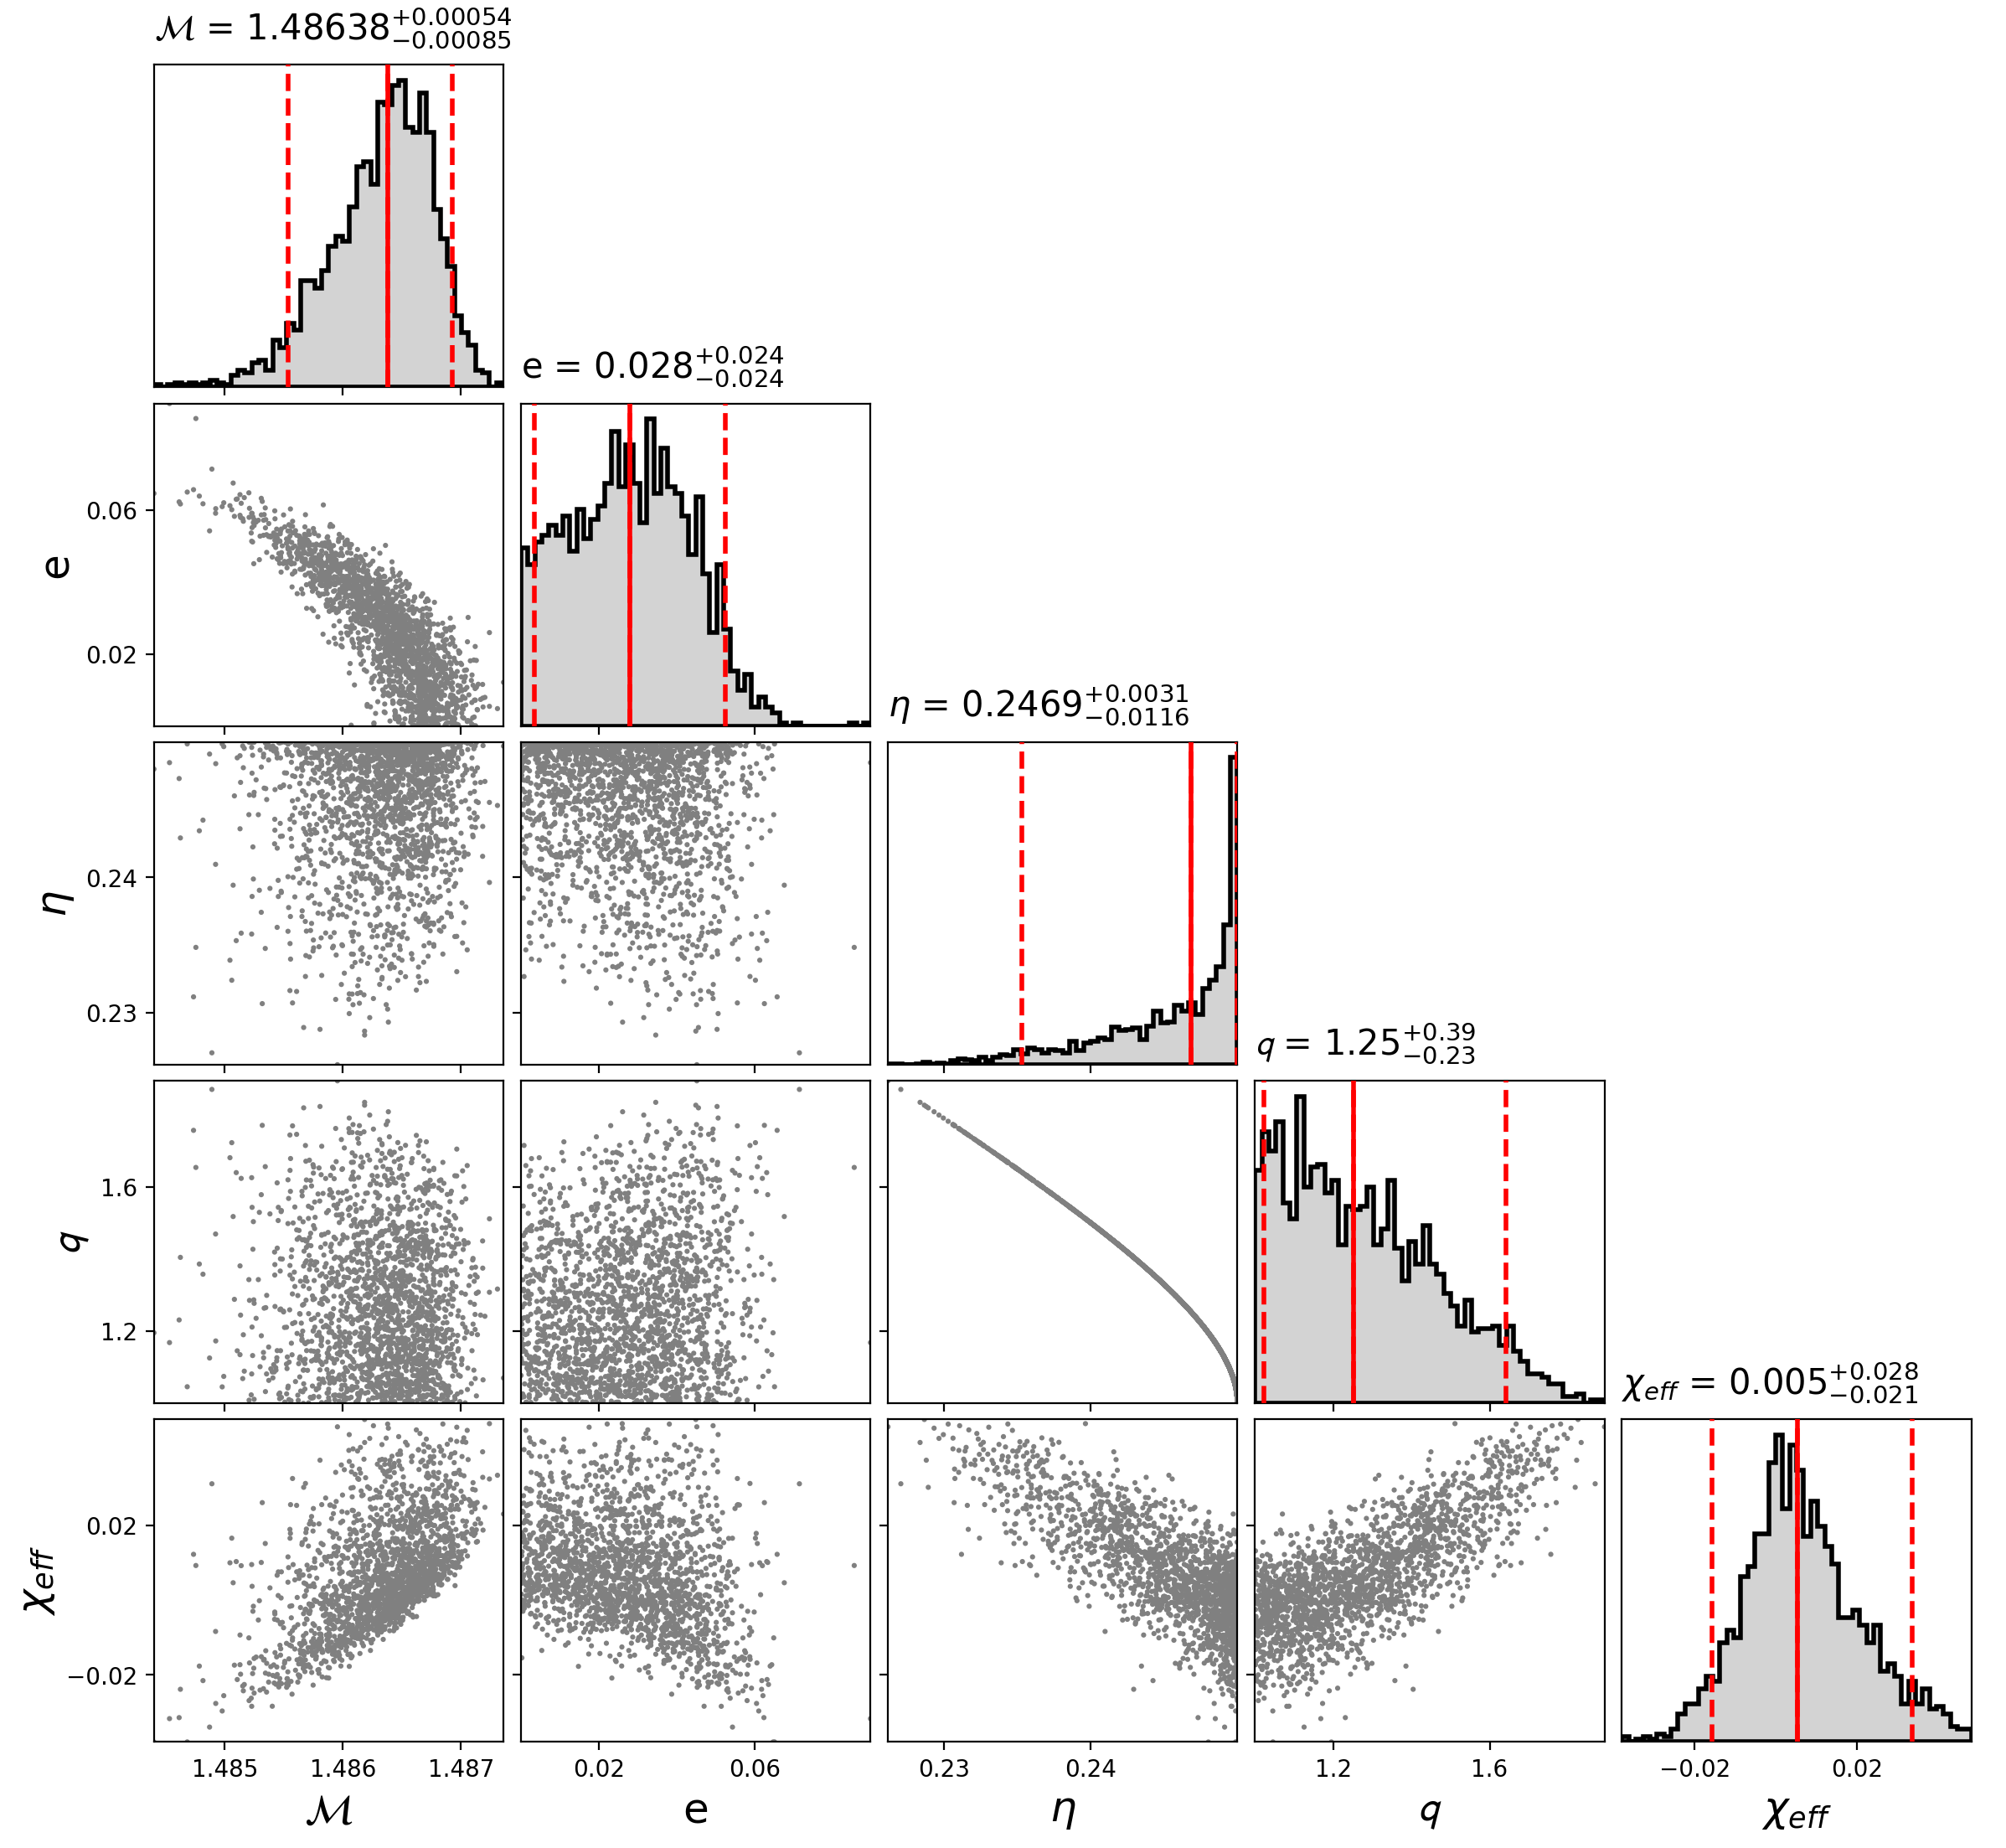
\includegraphics[width=\textwidth]{Figures/bns-pe/GW190425-e10.png}
    \caption{Posterior probability distribution of GW190425 at 10 Hz. The analysis used a prior uniform in $\ecc$. Each parameter is quoted with a median value (solid red line) and a 90\% credible interval (dashed red lines). The chirp mass $\mathcal{M}$ is given in the detector frame. Note the degeneracy between $\chirpm$ and $\ecc$.}
\label{Fig:GW190425}
\end{figure}

\begin{figure}[p]
    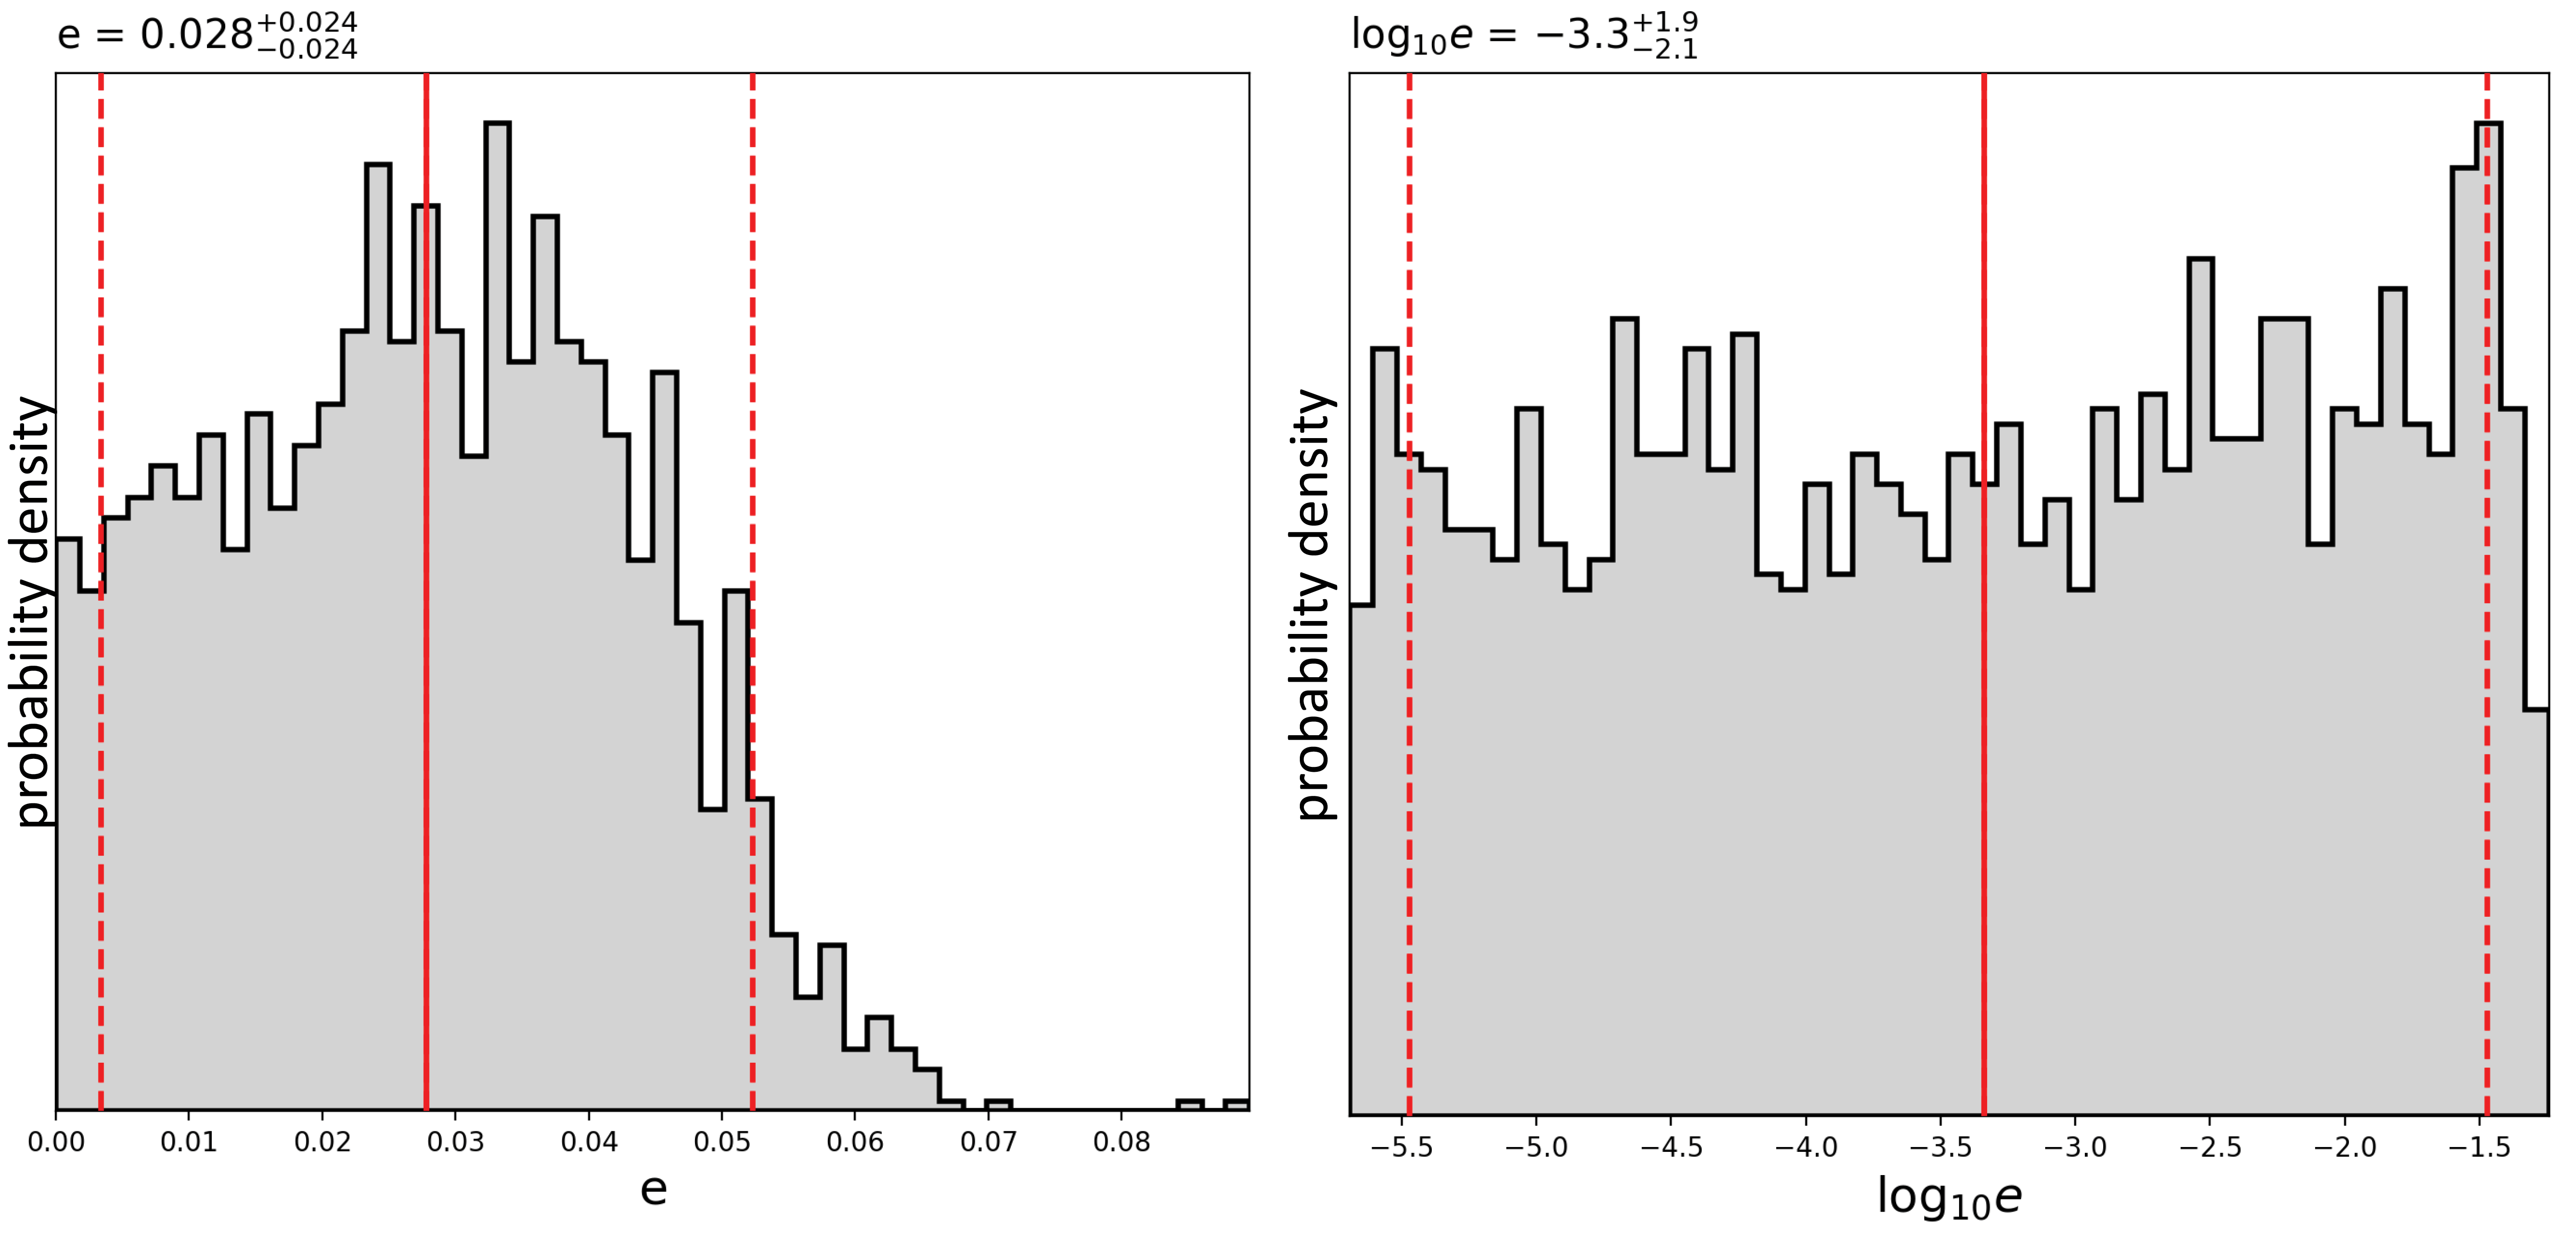
\includegraphics[width=\textwidth]{Figures/bns-pe/1Dmarginal-eccen-10hz.png}
    \caption{Eccentricity posteriors of GW190425 (solid black line) plotted against their priors (dotted line) for two choices of prior: uniform in $\ecc$ (left) and uniform in $\log_{10}(e)$ (right). We quote the median (solid red line) and 90\% credible interval (dashed red lines) for e in each posterior. The prior uniform in $\log_{10}(e)$ has the same distribution as the prior used in the Ref.~\protect\cite{Romero-Shaw:2020aaj} analysis.}
    \label{Fig:1DMarginal}
\end{figure}
\Chapter{Eccentric Binary Neutron Star Search Prospects for Cosmic Explorer}
\label{ch:3G-eccen-prospects}
\section{\label{sec:3G-Intro}Introduction}

Cosmic Explorer is a proposed third-generation gravitational-wave observatory that will have an order of magnitude improved sensitivity beyond that of Advanced LIGO and will be able to explore gravitational-wave frequencies below 10~Hz~\cite{Reitze:2019iox}. Cosmic Explorer will be able to detect binary neutron stars with a signal-to-noise ratio of $\ge 8$ out to a distance of $\sim 2$~Gpc~\cite{Chen:2017wpg}. Although most of the detected neutron-star binaries will be in circular orbits, measurement of eccentricity in neutron-star mergers allows us to explore their formation and to distinguish between field binaries, which are expected to be circular by the time they are observed~\cite{Peters:1964}, and binaries formed through other channels~\cite{Smarr1976,Canal:1990dz,PortegiesZwart1:1997zn,Postnov:2006hka,Kalogera:2006uj,Kowalska:2010qg,Beniamini:2015uta,Tauris:2017omb,Palmese:2017yhz,Belczynski:2018ptv,Vigna-Gomez:2018dza,Giacobbo:2018etu,Mapelli:2018wys,Andrews:2019vou}.

Dynamical interactions can form binary neutron stars with eccentricity that is measurable, although the predicted rate of these mergers detectable by current gravitational-wave observatories is small~\cite{Lee:2009ca,Ye:2019xvf}. The two binary neutron star mergers observed by Advanced LIGO and Virgo \cite{TheLIGOScientific:2017qsa,Abbott:2020uma} were both detected with searches that use circular waveform templates \cite{Allen:2004gu,Allen:2005fk,Canton:2014ena,Usman:2015kfa,Nitz:2017svb,Sachdev:2019vvd,Cannon:2020qnf,Davies:2020tsx, DalCanton:2020vpm}. Constraints have been placed on the eccentricity of these binaries. At a gravitational-wave frequency of 10 Hz, the eccentricity of GW170817 is $e_{10} \leq 0.024$~\cite{Lenon:2020oza} and GW190425 has an eccentricity $e_{10} \leq 0.048$~\cite{Romero-Shaw:2019itr, Lenon:2020oza} (90\% confidence). Ref.~\cite{Romero-Shaw:2019itr} considered unstable mass transfer as a formation scenario for GW190425, but the measured eccentricity limit was insufficient to confirm this hypothesis. A search for eccentric binary neutron stars in the first and second Advanced LIGO and Virgo observing runs did not yield any candidates~\cite{Nitz:2019spj}.

By extrapolating the upper limit on the rate of eccentric binary neutron stars from LIGO--Virgo observations, Ref.~\cite{Nitz:2019spj} estimates that the A+ upgrade~\cite{Aasi:2013wya} of Advanced LIGO will require between half a year of observation and $\sim 775$ years of observation before the detectable rate is comparable with the optimistic~\cite{Lee:2009ca} and pessimistic~\cite{Ye:2019xvf} rate predictions respectively, and an observation is plausible.  However, with its increased sensitivity and bandwidth, Cosmic Explorer would need at most half a year of observations to achieve a detectable rate comparable to even the pessimistic models~\cite{Nitz:2019spj}.

We investigate the ability of Cosmic Explorer to detect eccentric binary neutron stars and to measure their eccentricity. We find that at an eccentricity $e_{7} = 0.004$, a matched-filter search using circular waveform templates begins to lose more than $3\%$ of the signal-to-noise ratio due to mismatch between the circular and eccentric waveforms; this is an order of magnitude smaller than the equivalent limit for Advanced LIGO~\cite{Brown:2009ng,Huerta:2013qb}. We demonstrate that stochastic template placement \cite{Harry:2009ea,Manca:2009xw} can be use to construct a template bank that maintains a fitting factor greater than 97\% to binaries with $e_{7} \le 0.05$. We will reference eccentricity at a reference frequency of We will use a reference frequency of $7$~Hz in reference to eccentricity unless otherwise stated.

Using template banks constructed for Cosmic Explorer, we estimate the computational cost of matched-filter searches for binary neutron stars in circular and eccentric orbits and find that both are accessible with present-day computational resources. We then estimate the ability of Cosmic Explorer to measure and constrain the eccentricity of detected binary neutron star systems. For a binary neutron star with signal-to-noise ratio 8 (800), Cosmic Explorer will be able to measure eccentricities $\gtrsim 8\times 10^{-3}$ ($8\times 10^{-4}$). 

This paper is organized as follows: In Sec.~\ref{s:3G-circ}, we investigate the ability of a matched-filter search to detect eccentric binary neutron stars in Cosmic Explorer. We calculate the lower-frequency cutoff required to obtain at least $99.9\%$ of the available signal-to-noise ratio for binary neutron stars ($m_{1,2} \in [1,3]\,\mathrm{M}_\odot$). Using this frequency cutoff, we use geometric placement to construct a template bank using circular waveform for Cosmic Explorer that has a fitting factor of $97\%$ and estimate the computational cost of performing a matched-filter search using this bank. In Sec.~\ref{s:3G-ecc} we measure the loss in fitting factor when using a bank of circular waveform with neutron-star binaries with eccentricity $e \le 0.05$. We use stochastic template placement to generate a bank containing circular and eccentric waveforms than has a fitting factor of $96.5\%$ and estimate the computational cost of this eccentric binary search. In Sec.~\ref{s:3G-pe}, we estimate the minimum eccentricity that can be measured by Cosmic Explorer as a function of the signal-to-noise ratio of the detected signal. We compare this to estimates of Advanced LIGO and the eccentricity constraints placed by the detection of GW170817. Finally, in Sec.~\ref{s:3G-conc}, we discuss the implications our results for measurement of eccentric binaries with Cosmic Explorer and extension of our work to higher eccentricities and binary black holes.


\section{\label{s:3G-circ} Binary Neutron Star Searches in Cosmic Explorer}

Cosmic Explorer has a two-stage design~\cite{Reitze:2019dyk, Reitze:2019iox}. The first stage of Cosmic Explorer (CE1) assumes that the detector's core technologies will be similar to those of Advanced LIGO with the sensitivity gain from increasing the detector's arm length from 4~km to 40~km. The second stage (CE2) is a technology upgrade to the CE1 detector that further increases Cosmic Explorer's sensitivity. Estimates of the detector's noise power spectral density $S_n(f)$ are available for both CE1 and CE2~\cite{CE:NoiseCurves}; we consider both detector configurations in our analysis. 

Compared to the low-frequency sensitivity limit of Advanced LIGO, which lies around $10$~Hz, Cosmic Explorer pushes the low-frequency limit of the detector below this limit~\cite{Reitze:2019iox}. As for Advanced LIGO, the detector noise begins to rapidly increase as the gravitational-wave frequency reaches the seismic and Newtonian noise walls at low-frequency. The length of a binary neutron star waveform has a steep power-law dependence on its starting frequency $f_\mathrm{lower}$, with the number of cycles between $f_\mathrm{lower}$ and the coalescence frequency scaling as $f_\mathrm{lower}^{-8/3}$. A binary neutron star waveform that starts at $f_\mathrm{lower} = 3$~Hz has a length of approximately $7$~hours, presenting non-trivial data analysis challenges in searches and parameter estimation. 

To determine the optimal starting frequency for binary neutron star searches in Cosmic Explorer, we consider the accumulation of the the signal-to-noise ratio in a matched filter search for a neutron star binary with $m_1 = m_2 = 1.4\,M_\odot$; this accumulates linearly with frequency $f$ as $f^{-7/3} / S_n(f)$~\cite{Finn:2000hj,Allen:2005fk}. Fig.~\ref{Fig:comp-cost-SNRfrac} shows the fraction of the total signal-to-noise ratio accumulated at a given frequency for Cosmic Explorer and Advanced LIGO. Advanced LIGO's most sensitive frequency lies around 40~Hz with almost no detectable signal below 10~Hz. For CE1 and CE2, the peak sensitivity of the detectors to binary neutron stars is shifted to lower frequencies, with a non-trivial amount of signal-to-noise available below 10~Hz.
The fraction of signal-to-noise available drops rapidly as the frequency decreases due to the low-frequency noise wall of Cosmic Explorer.
\begin{figure}
    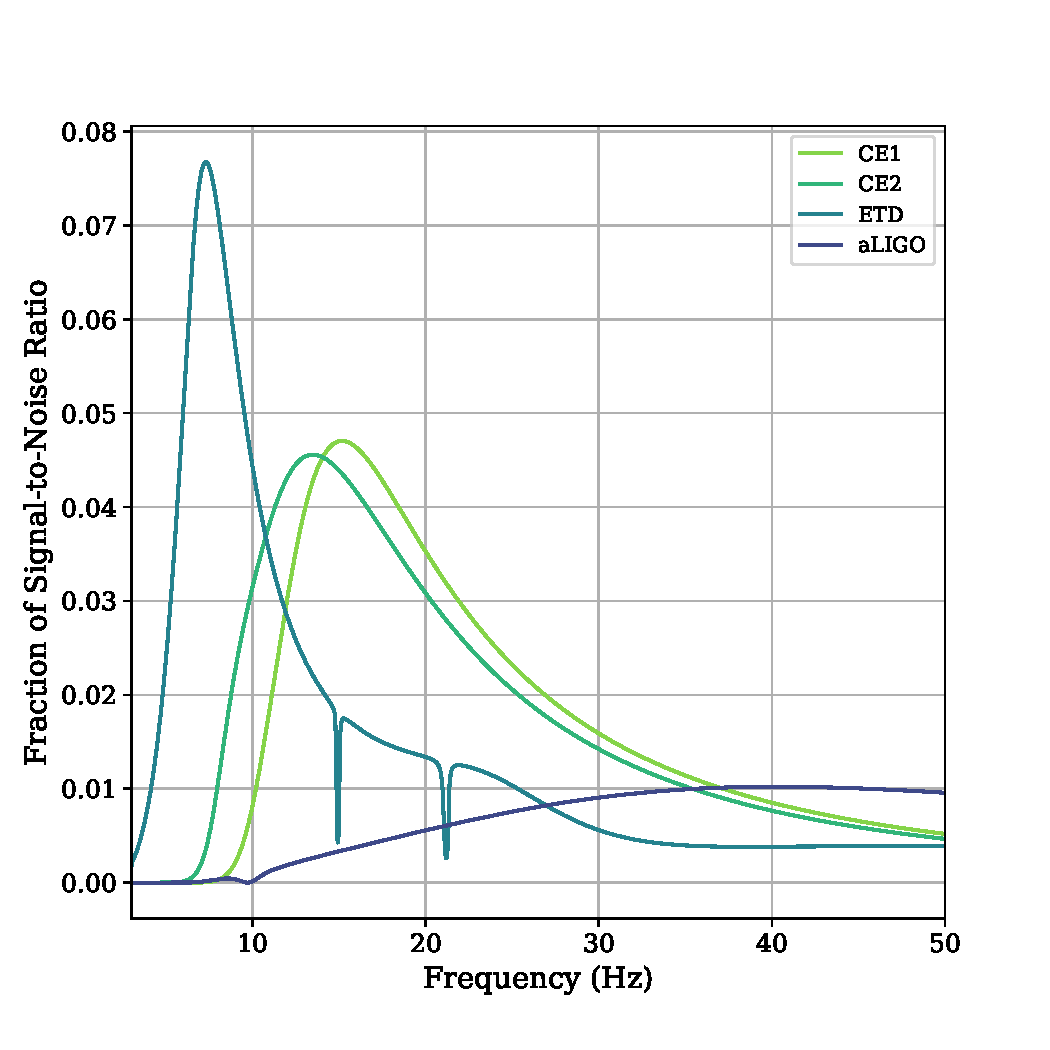
\includegraphics[width=1.1\columnwidth]{Figures/3G-bns-search-prospects/SNRfraction-compcost.pdf}
    \caption{The fraction of signal-to-noise ratio as a function of frequency for Cosmic Explorer (CE1/CE2), Einstein Telescope (ETD) and Advanced LIGO (aLIGO). This gives a visual representation of what the matched filter sees when it is integrating up the signal-to-noise ratio. A majority of the signal-to-noise ratio for Cosmic Explorer and Advanced LIGO is accumulated between 10 and 50~Hz, while the signal-to-noise ratio for Einstein Telescope is accumulated below 10~Hz.}
\label{Fig:comp-cost-SNRfrac}
\end{figure}

To determine the optimal low-frequency cutoff, we consider the cumulative fraction of the total signal-to-noise ratio as a function of low-frequency cutoff, shown in Fig.~\ref{Fig:comp-cost-cumulSNR}. This is computed by comparing the ratio of the signal-to-noise obtained by integrating from $3$~Hz to a fiducial low-frequency cutoff shown on the ordinate of Fig.~\ref{Fig:comp-cost-cumulSNR}.
We find that for both the CE1 and CE2 detector sensitivity curves, the matched filter accumulates 99.97\% (99.53\%) of the signal-to-noise above 7~Hz for CE1 (CE2). We therefore use 7~Hz as an appropriate low-frequency cutoff for our analysis. At this starting frequency, the length of a binary neutron star waveform is reduced by two orders of magnitude to $4600$~s (77 minutes). For a
waveform of this length, the Doppler frequency modulation due to the diurnal
and orbital motion is $(\Delta f / f ) \sim 10^{-8}$ and can be neglected in
search algorithms. Similarly, the time dependence of the antenna response due to the Earth's rotation can be neglected as the match between a waveform that neglected the time variation and a waveform that accounted for the variation is 98-99\%. For comparison, we show the same result for the proposed E.U. third-generation detector Einstein Telescope~\cite{Maggiore:2019uih}. Einstein Telescope has a significantly lower seismic--Newtonian-noise wall than Cosmic Explorer and so searches must be pushed to lower frequencies to accumulate all of the possible signal-to-noise ratio. We focus on Cosmic Explorer in this work as we have found that existing methodologies are sufficient to effectively address the challenges presented by the increased low-frequency sensitivity of the third generation observatory.  Einstein Telescope has a significantly lower seismic--Newtonian-noise wall than Cosmic Explorer and so searches must be pushed to lower frequencies to accumulate all of the possible signal-to-noise ratio. For an optimal search of Einstein Telescope, this may require addressing how to best account for the time-dependent detector response. 
\begin{figure}
    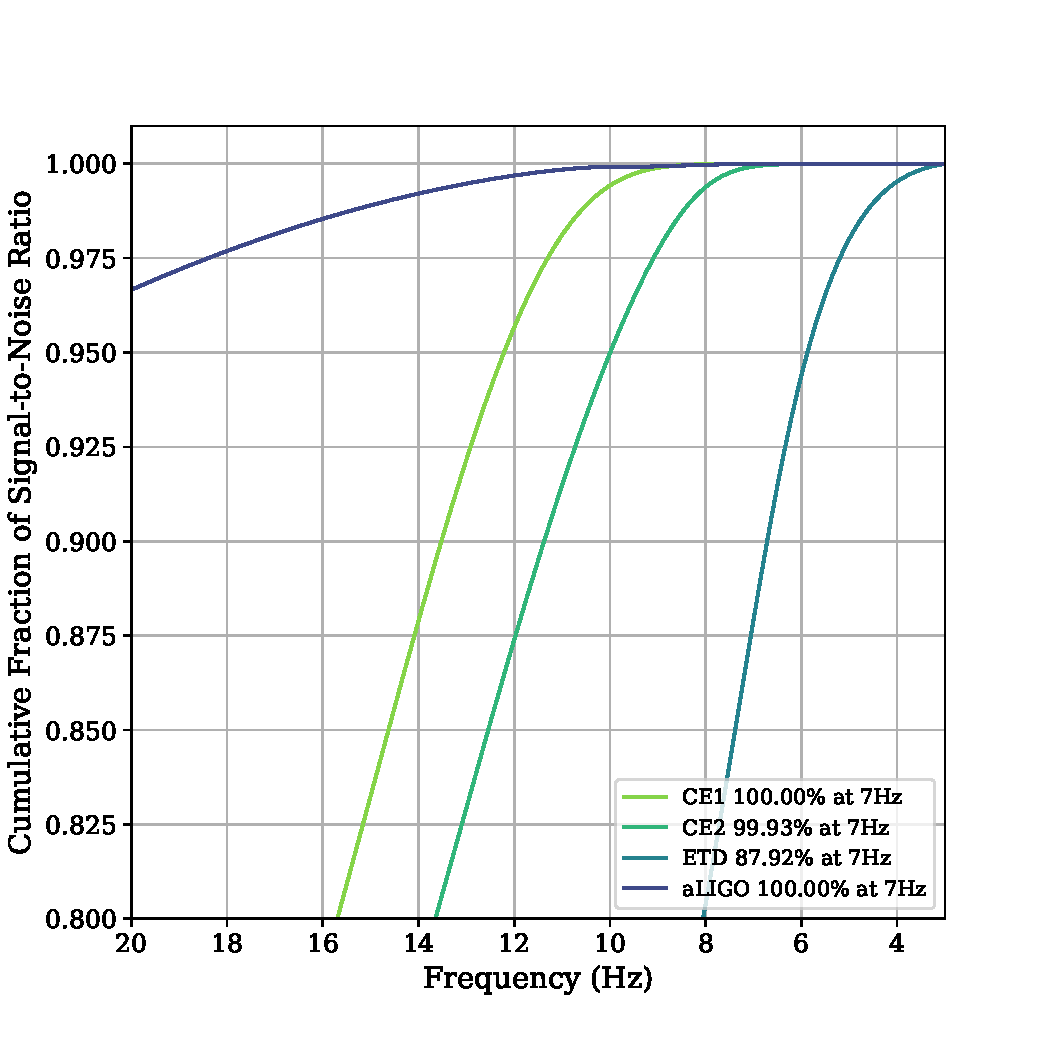
\includegraphics[width=1.1\columnwidth]{Figures/3G-bns-search-prospects/cumul-SNR-compcost.pdf}
    \caption{The cumulative fraction of signal-to-noise ratio as a function of frequency. Cosmic Explorer (CE1/CE2) and Advanced LIGO (aLIGO) have accumulated more than 99.9\% of their total signal-to-noise ratio from frequencies above 7~Hz. At 7~Hz, Einstein Telescope (ETD) accumulated more than 85\% of their total signal-to-noise ratio. Since more than 99.9\% of the total signal-to-noise ratio is accumulated, we use a low-frequency cutoff of 7~Hz to generate the waveforms in our template banks.}
\label{Fig:comp-cost-cumulSNR}
\end{figure}

Using a $7$~Hz low-frequency cutoff, we generate a template bank that can be used to search for binary neutron star merger with component masses $1.0 \leq m_1,m_2 \leq 3.0$. We first generate a template bank for binaries with zero eccentricity and component spin using the standard hexagonal lattice method of template placement~\cite{Owen:1995tm,Owen:1998dk,Cokelaer:2007kx,Brown:2012qf}. The template bank is constructed so that it has a fitting factor of $97\%$~\cite{Apostolatos:1995pj}. We find that the number of templates required for the CE1 (CE2) sensitivity is $130,000$ ($209,000$) to achieve a fitting factor of $97\%$. A template bank generated using the Advanced LIGO sensitivity and a $10$~Hz low-frequency cutoff contains $77,000$ points. Since the CE1 (CE2) template banks are only a factor of 1.7 (2.8) larger than the equivalent template bank for Advanced LIGO, we do not expect significant computational challenges executing these searches. We certainly expect no obstacles to implementing real-time searches a decade or more from now when Cosmic Explorer will be operational.

Before constructing a template bank for binaries with eccentricity, we determine how effective the non-eccentric template bank is at detecting signals from eccentric binary neutron star sources. We perform the standard test of measuring the match between a random set of eccentric gravitational-wave signals and maximizing this over the template bank to obtain the bank's fitting factor to a population of eccentric signals. To model eccentric sources, we use the LIGO Algorithm Library implementation \cite{lalsuite} of TaylorF2Ecc, a frequency-domain post-Newtonian model with eccentric corrections. This waveform is accurate to 3.5 pN order in orbital phase \cite{Buonanno:2009zt}, 3.5 pN order in the spin-orbit interactions \cite{Bohe:2013cla}, 2.0 pN order in spin-spin, quadrupole-monopole, and self-interactions of individual spins \cite{Mikoczi:2005dn,Arun:2008kb}, and 3.0 pN order in eccentricity \cite{Moore:2016qxz}. To model non-eccentric waveforms, we use the restricted TaylorF2 approximant, accurate to the same post-Newtonian order.

We test the template bank against $120,000$ simulated signals that have detector-frame component masses $1.0 \leq m_1,m_2 \leq 3.0$ and eccentricity $0 \le e \le 0.05$. The results of the simulation are shown in Fig.~\ref{Fig:ff-circ-CE1} and Fig.~\ref{Fig:ff-circ-CE2} for CE1 and CE2, respectively. If the population of neutron star binaries has eccentricity less than 0.004 (0.003) in CE1 (CE2), then the non-eccentric template banks achieve a fitting factor of $97\%$ and are effectual. However, for sources with larger eccentricities the effectualness of the template bank begins to rapidly decline; the effectualness of a non-eccentric binary neutron star bank fails at an eccentricity an order of magnitude lower than that of Advanced LIGO~\cite{Brown:2009ng, Huerta:2013qb}. To recover these signals, it is necessary to construct a template bank that captures eccentricity. We consider this in the next section.
\begin{figure}
    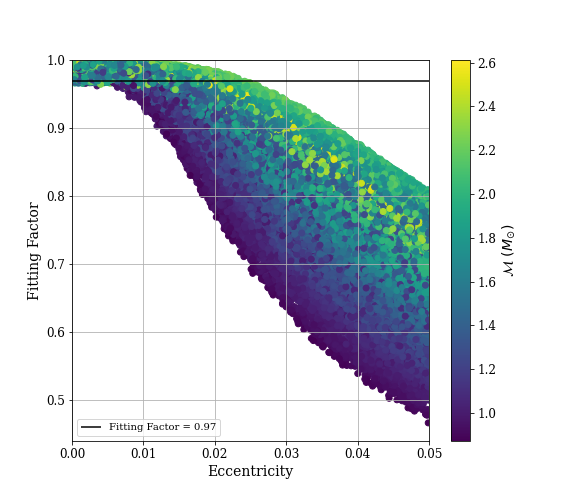
\includegraphics[width=1.1\columnwidth]{Figures/3G-bns-search-prospects/non-eccen-ff-mchirp-CE1.png}
    \caption{The fitting factor as a function of eccentricity correlated with chirp mass for CE1. A non-eccentric template bank was used to calculate the fitting factor. For Cosmic Explorer the fitting factor decreases for increasing values of eccentricity. The non-eccentric template bank is effective in detecting eccentric systems with a fitting factor greater than 97\% for $\ecc \lesssim 0.004$.}
\label{Fig:ff-circ-CE1}
\end{figure}
\begin{figure}
    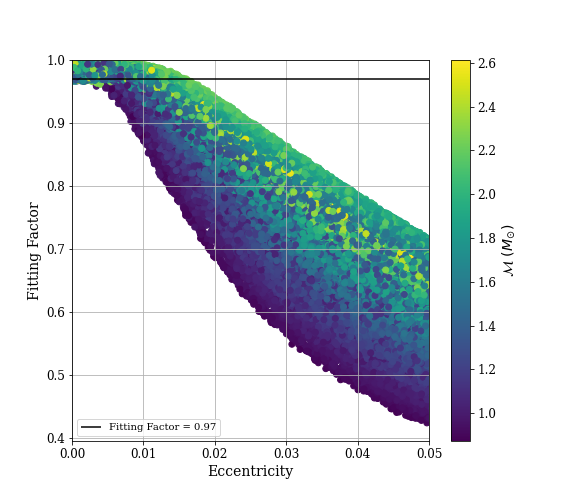
\includegraphics[width=1.15\columnwidth]{Figures/3G-bns-search-prospects/non-eccen-ff-mchirp-CE2.png}
    \caption{As in Fig.~\ref{Fig:ff-circ-CE1}, but we use the CE2 noise curve. A non-eccentric template bank was used to calculate the fitting factor. The non-eccentric template bank is effective in detecting eccentric systems with a fitting factor greater than 97\% for $\ecc \lesssim 0.003$.}
\label{Fig:ff-circ-CE2}
\end{figure}

\section{\label{s:3G-ecc} Extension to Eccentric Template Banks}

The number of templates in an eccentric bank will depend on the bandwidth of the detector and the upper eccentricity boundary of the bank. To visualize the dependency on detector bandwidth , Fig.~\ref{Fig:eccen-lim} shows the eccentricity ambiguity function for a $m_1 = m_2 = 1.4~\msun$ binary. This shows how quickly the loss in signal-to-noise ratio (match) changes as the  eccentricity increases from $0$ to $0.4$ (referenced to 7~Hz). Without the use of eccentric templates, the match for CE1 (CE2) decreases to 34\% (30\%) at $e = 0.05$. In contrast, the Advanced LIGO match decreases much more slowly, reaching 38\% at $e = 0.4$. Consequently, the density of an eccentric template bank will be significantly greater for Cosmic Explorer than Advanced LIGO.

Searches for eccentric binary neutron stars in Advanced LIGO used a template bank that covers the eccentricity range $0 \le e \le 0.4$ (referenced to 10~Hz)~\cite{Nitz:2019spj}; this bank contained $350,000$ templates. To generate template banks of comparable density in eccentricity for Cosmic Explorer, we set the upper eccentricity of the template bank to $e=0.05$ and keep the mass boundaries at $1.0 \leq m_1,m_2 \leq 3.0$ and the lower-frequency cutoff at 7~Hz. We then generated a template bank for eccentric gravitational-wave signals in this region using the stochastic placement method~\cite{Harry:2009ea,Manca:2009xw} with a fitting factor of $96.5\%$. 
\begin{figure}
    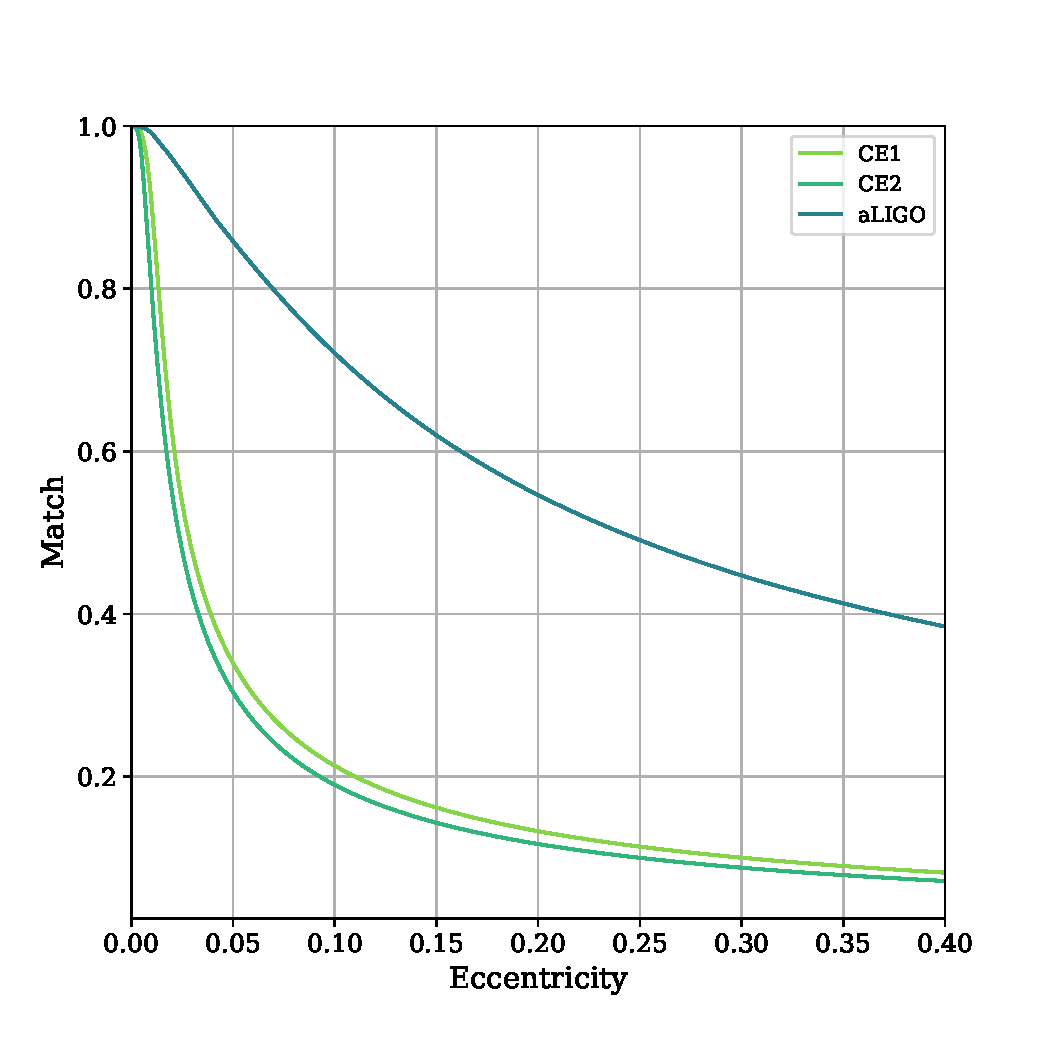
\includegraphics[width=1.1\columnwidth]{Figures/3G-bns-search-prospects/eccen-limit.pdf}
    \caption{The match as a function of eccentricity for Cosmic Explorer (CE1/CE2) and Advanced LIGO (aLIGO). This gives a representation of the match between an circular waveform and an eccentric waveform for various eccentricities. The match for Cosmic Explorer at an eccentricity of 0.05 is about a factor of 3 smaller than that of Advanced LIGO.}
\label{Fig:eccen-lim}
\end{figure}

We test the eccentric template bank against $25,000$ simulated signals with detector-frame component masses uniformly distributed between $1.0 \leq m_1,m_2 \leq 3.0$ and eccentricity uniformly distributed between $0 \le e \le 0.05$. The resulting fitting factor of these bank is shown in Fig.~\ref{Fig:cumul-hist}, with the fitting factor of the non-eccentric bank as reference. This result shows that the stochastic bank placement is effectual for signals with eccentricity in the target region, as all signals can be recovered with a fitting factor of $\gtrsim 95\%$ both the CE1 and CE2 banks. The number of eccentric templates generated using the CE1 (CE2) sensitivity is $1,900,000$ ($6,400,000$), an order of magnitude larger than the non-eccentric template banks for CE and an order of magnitude larger than the the Advanced LIGO eccentric bank. We consider the size of a template bank with $e_{max} = 0.1$ to determine the increase in templates as eccentricity increases. A template bank with $0 \le e \le 0.1$ has $4,500,000$ templates using the CE1 sensitivity, this is twice the size of the template bank we consider in this work. We expect that a bank of this size will present no computational challenges when Cosmic Explorer is operational in the 2030s; searches of similar magnitude are already regularly performed~\cite{Nitz:2020bdb, Nitz:2021mzz}.  

\begin{figure}
    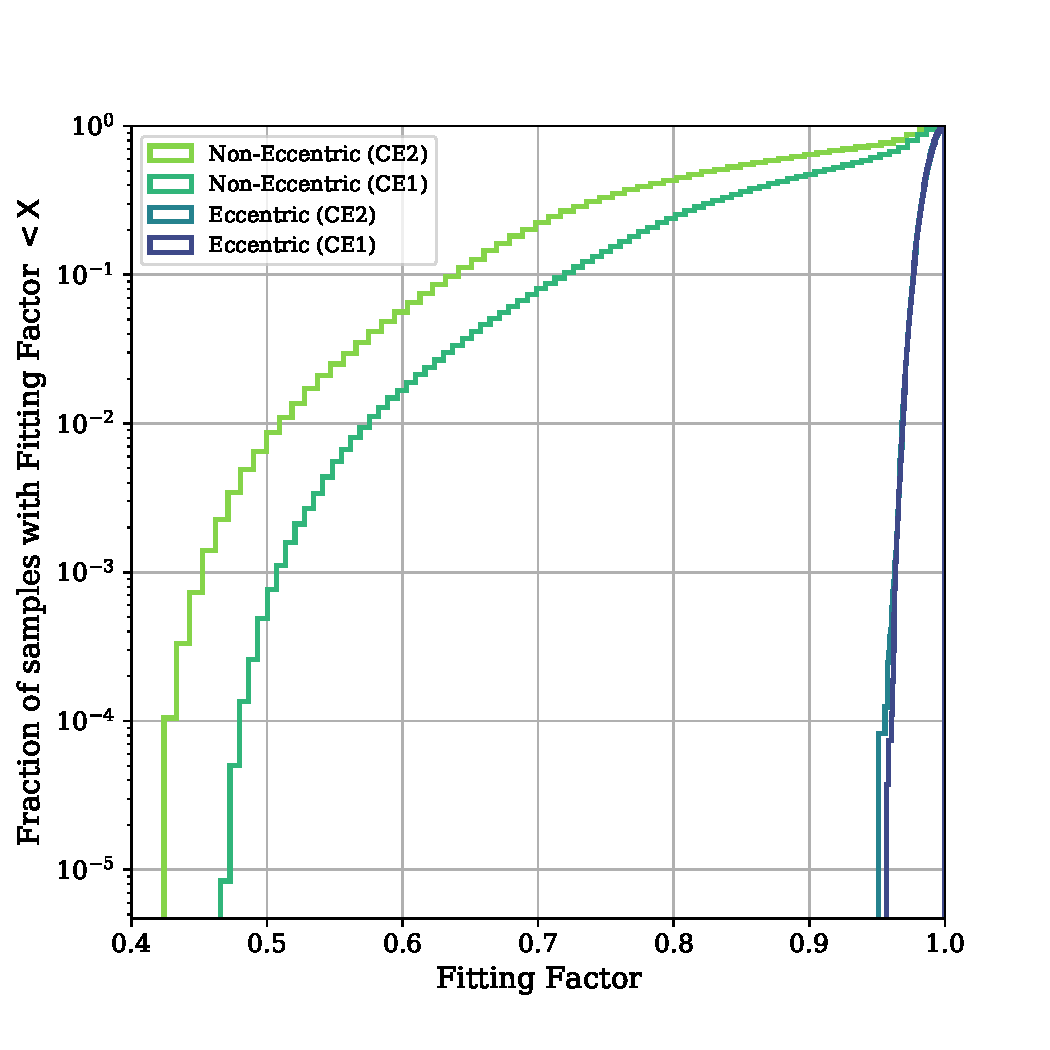
\includegraphics[width=1.1\columnwidth]{Figures/3G-bns-search-prospects/cumhist-ff-CB.pdf}
    \caption{A cumulative histogram that shows the fraction of points where the fitting factor is less than the value on the x-axis for each template bank. Using the eccentric template bank, a majority of the samples are at a fitting factor $\gtrsim 95\%$. For our eccentricity range, the eccentric template banks appear to do a better job at detecting eccentric systems than the non-eccentric template banks.}
\label{Fig:cumul-hist}
\end{figure}
        
\section{\label{s:3G-pe}Binary Neutron Star Parameter Estimation in Cosmic Explorer}

We can use our results to estimate the constraints that Cosmic Explorer will be able to place on the eccentricity of detected binary neutron stars with parameter estimation. We express this as the signal-to-noise ratio required to distinguish between an eccentric and circular binary at 90\% confidence. This can be interpreted as the minimum detectable eccentricity at a given signal-to-noise ratio, or the upper limit that can be placed on the eccentricity of a circular a binary detected at a given signal-to-noise ratio.

To estimate this signal-to-noise required to distinguish between a circular binary and a binary with eccentricity $e$ at 90\% confidence, we use the method of Baird {\it et al.}~\cite{Baird:2012cu}. This method relies on the fact that parameter estimation identifies regions of parameter space where a waveform is most consistent with the data. Ref.~\cite{Baird:2012cu} uses the fact that high confidence regions in parameter estimation are associated with regions of high match between signal and template to obtain a relationship between the match and signal-to-noise ratio $\rho$, given by
\begin{equation}
    M(h(\theta),h(\langle\theta\rangle)) \geq 1 - \frac{\chi_k^2(1-p)}{2\rho^2}
    \label{eq:baird}
\end{equation}
where $k$ is the dimension of the parameter space of interest, $\chi^2(1 - p)$ is the chi-square value for which there is $1 - p$ probability of obtaining that value or larger. Here, we set $k=4$ corresponding to intrinsic parameter space of an aligned spin binary neutron star merger with eccentricity ($m_1, m_2, \chi_\mathrm{eff}, e$), where $\chi_\mathrm{eff}$ is the effective spin of the binary, and $p = 0.9$ for 90\% confidence.

For Eq.~(\ref{eq:baird}) to provide a reasonable estimate of the signal-to-noise ratio, the match $M$ must be maximized over the parameters of the signal. For eccentric binaries, there is a known degeneracy between the chirp mass $\mathcal{M} = (m_1  m_2)^{3/5} / (m_1 + m_2)^{1/5}$ of the binary and the eccentricity~\cite{Martel:1999tm,Lenon:2020oza}. Full parameter estimation naturally explores the likelihood and this degeneracy. Here, we use our method of eccentric template placement to place a fine grid of templates and brute-force maximize the match over this template bank to account for the chirp mass--eccentricity degeneracy.

Using this method, we estimate Cosmic Explorer's ability to constrain the eccentricity of a $m_1 = m_2 = 1.4\,\msun$ binary as follows: Using a low frequency cutoff of $7$~Hz, we generate a template bank with binary neutron star component masses $1.399 \leq m_1,m_2 \leq 1.401$, eccentricity $0 \leq e \leq 0.05$, an upper-frequency cutoff of $4096$~Hz, and a minimal match of 99.9999\%. We measure the match between a simulated eccentric gravitational-wave signal with component masses $m_1 = m_2 = 1.4$ and eccentricity $0 \leq e \leq 0.05$ and maximize over the chirp mass in the template bank to get the signal-to-noise ratio. From this we determine the signal-to-noise ratio needed to reach a 90\% confidence interval~\cite{Baird:2012cu} to measure the eccentricity.

We apply the above method using the CE1, CE2, and Advanced LIGO design noise curves to obtain the signal-to-noise ratio as a function of eccentricity required to distinguish between a circular and eccentric binary. To check the accuracy of our estimation, we also compute this function using the detector noise around the time of GW170817 and compare the Baird {\it et al.} estimate to the 90\% upper limit on the eccentricity of GW170817 computed using full parameter estimation~\cite{Lenon:2020oza}. These result are shown in Fig.~\ref{Fig:SNRvEccen}. First, we note that our method provides a reasonable approximation when comparing to GW170817 and as the eccentricity increases the signal-to-noise ratio needed to resolve the signal decreases, as expected. Our results suggest that for $e \geq 8\times10^{-3}$ ($8\times 10^{-4}$), a minimum signal-to-noise ratio of 8 (800) would be needed to resolve the signal at 90\% confidence in CE1 and CE2. This is an order of magnitude better than expected from Advanced LIGO operating at design sensitivity.

\begin{figure}
    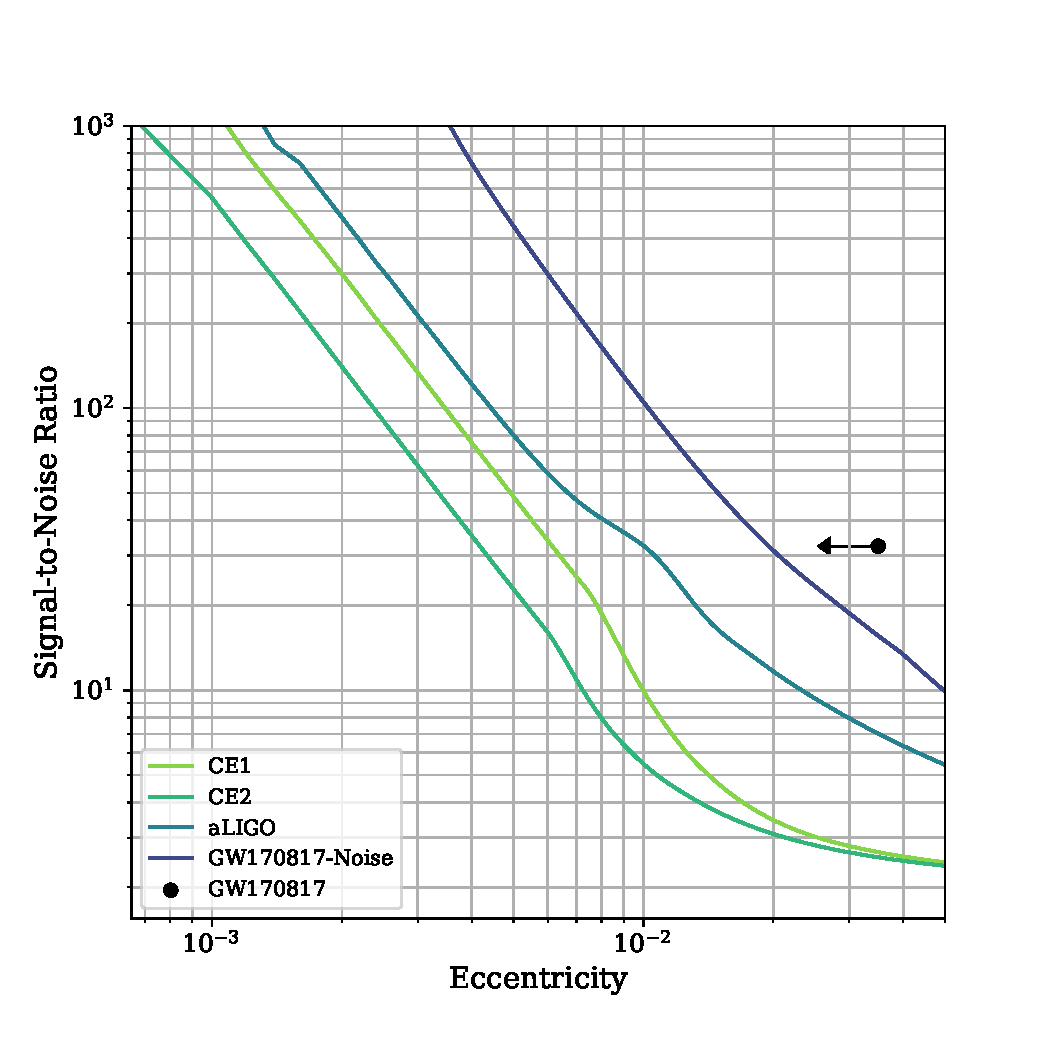
\includegraphics[width=1.1\columnwidth]{Figures/3G-bns-search-prospects/SNR-loglog-e7.pdf}
    \caption{The signal-to-noise ratio as a function of eccentricity. The black dot is at an signal-to-noise ratio of $32.4$~\cite{TheLIGOScientific:2017qsa} and eccentricity of 0.024 at 90\% confidence~\cite{Lenon:2020oza}. For each detector, we show the signal-to-noise ratio needed to resolve the signal with eccentricity on the x-axis at 90\% confidence. For $e \geq 10^{-3}$, a signal-to-noise ratio of 8 would be needed to resolve the signal at 90\% confidence in Cosmic Explorer. As the eccentricity decreases, the signal-to-noise ratio needed to resolve the signal increases.}
\label{Fig:SNRvEccen}
\end{figure}

\section{\label{s:3G-conc}Conclusion}

Our analysis used circular and eccentric template banks to determine the ability of Cosmic Explorer to detect eccentric binary neutron stars and to measure their eccentricity. The circular template banks are effective for detecting eccentric binaries with $e \leq 0.004$ ($e \leq 0.003$) in CE1 (CE2) at a reference frequency of $7$~Hz. However, for larger eccentricities a template bank containing circular and eccentric waveform templates is required. This estimate is an order of magnitude smaller than estimates for Advanced LIGO~\cite{Brown:2009ng, Huerta:2013qb}. We determine the signal-to-noise ratio needed to constrain the eccentricity of a detected neutron star binary signal with 90\% confidence. We also find that in Cosmic Explorer to measure binary neutron star with eccentricity $\gtrsim 8\times 10^{-3}$ ($8\times 10^{-4}$) a signal-to-noise ratio of 8 (800) is needed to resolve the signal at a reference frequency of $7$~Hz (90\% confidence). Accurately constraining the eccentricity of the binary would provide valuable information on the formation of these mergers.

The computational cost of searches with template banks containing higher eccentricities will be challenging in Cosmic Explorer today as the density of the template bank increases with increasing eccentricity (see Fig. 2 of Ref.~\cite{Nitz:2019spj}). However, improvements in technology by the 2030s may make these searches a possibility. Along with the high computational cost, current waveform models for eccentricity break down for $e \geq 0.4$. To accurately search for higher eccentricity neutron-star binaries models that extend to high eccentricities will need to be developed or a burst search will need to be used. To extend this work to binary black holes, waveforms that better model the merger--ringdown will need to be accessible~\cite{Tanay:2016zog, Huerta:2016rwp, Cao:2017ndf, Huerta:2017kez, Hinder:2017sxy} and will be left for future work. Understanding the constraints that future observational limits place on eccentric binary formation channels will require computation of the rate as a function of eccentricity from population synthesis. As Cosmic Explorer will be able to aid in the understanding of the physics of binary neutron star mergers it is important to accurately constrain the eccentricity as the number of mergers increases.

\Chapter{Conclusions}
\label{ch:conclusions}
In the current era of gravitational-wave astrophysics we are moving beyond first direct detections and first multimessenger observations, to now making routine discoveries that deepen our understanding of the compact objects in our cosmic neighborhood. The LIGO-Virgo gravitational-wave detector network has detected 52 confirmed binary merger observations so far, and the detection rate has only accelerated as improved detector sensitivity extends our reach deeper into the universe. From the two observed binary neutron star mergers, our knowledge of the dynamics of these events and of neutron star physics has grown dramatically. They have provided confirmation of binary neutron star mergers as a source of short gamma-ray bursts, and also as important sites of heavy element production through $r$-process nucleosynthesis that can help explain observed chemical abundances. They have also shown that it is possible to measure the tidal information in a gravitational-wave signal to meaningfully update our constraints on the nuclear equation of state. As the LIGO-Virgo detectors approach their design sensitivity, and as third-generation detectors begin to come online, we expect to see many more binary neutron star mergers in the coming years. We anticipate that these new detections will provide even further insights into the physics of neutron stars.

In this thesis we have studied binary neutron star mergers, through a combination of observations and computational modeling. Specifically we explore the ability of a gravitational-wave analysis to extract physical parameters of the binary system, and of the neutron stars involved in the merger. We investigate the impact of multimessenger information on a gravitational-wave analysis, and we study the measurability of the nuclear equation of state, both now and in the future.

We have presented an analysis of the binary neutron star merger GW170817 informed by electromagnetic distance measurements of its identified host galaxy, and we demonstrated that using an independent distance measurement in a gravitational-wave analysis can break the distance-inclination degeneracy to allow for much tighter constraints on the inclination angle of the binary. We find our improved measurement of the inclination supports models for a structured relativistic jet and its afterglow emission being viewed off-axis.

We have presented measurements of the tidal deformabilities and radii of the neutron stars in GW170817. Our analysis imposed a physical constraint to require that both neutron stars obey the same equation of state, and we used a prior on the leading order tidal parameter constructed to contain all physical models of the equation of state without biasing the measurement toward any particular model. We note that the methodology we employed could be adapted for the analysis of future binary neutron star merger events with similar masses. We find our results are broadly consistent with several other studies~\cite{Abbott:2018exr,Radice:2018ozg,Coughlin:2018fis,Capano:2019eae} which employed various methods to measure the tidal deformabilities and radii in their own analyses of GW170817.

We have presented a likelihood model developed for \textit{PyCBC Inference} that uses the relative binning parameter estimation technique to reduce computational cost for potential multimessenger gravitational-wave sources. We extended the work of previous implementations to make our relative likelihood model a coherent network statistic so that it can additionally measure sky locations. We validated the relative model on populations of simulated binary neutron star and simulated neutron star--black hole merger signals, and we showed that it is possible to seed the relative analysis with the best-fit template parameters from a low-latency search pipeline. We found that the parameter estimation for all signals in our simulated populations completed in less than 20 minutes, with sky localization and intrinsic parameter estimates that are comparable to analyses done with a standard non-relative likelihood.

We have presented a comprehensive study of the future prospects for a precise equation of state measurement from Advanced LIGO and Cosmic Explorer. We explored the measurability of the equation of state across the full parameter space allowed by combined constraints from astrophysical observations and nuclear experiments. We showed that a precision threshold for measurements to distinguish between substantially similar theoretical models for the equation of state is equivalent to measuring the radius of a 1.4\msun\ neutron star to better than $2\%$, and we presented a framework for combining individual equation of state measurements across entire populations to produce a combined, high-precision measurement. We found it is unlikely that Advanced LIGO will achieve $2\%$ precision in the next observing runs given current estimates of the merger rate for binary neutron stars, however Cosmic Explorer will measure the equation of state to better than $1\%$ within one year of operation. Our framework can be directly applied to any future signals from binary neutron star mergers, and we anticipate that the resulting precise knowledge of the true equation of state will be invaluable for efforts to model these merger events and their associated kilonovae.
%\appendix
%\chapter{}
%\label{}
%\input{}
\clearpage
\bibliographystyle{unsrt}
\bibliography{eccentric-search-bib,bns-pe-bib,3G-eccen-prospects,references}
\addcontentsline{toc}{chapter}{\numberline {Bibliography}}

\renewenvironment{thebibliography}[1]%
  {\begin{list}{\labelenumi\hss}%
     {\usecounter{enumi}\setlength{\labelwidth}{3em}%
      \setlength{\leftmargin}{5em}}}%
  {\end{list}}
\renewcommand{\bibitem}[1]{\item\label{#1}\relax}%
\renewcommand{\theenumi}{\arabic{enumi}}%
%\fi
%\clearpage
%\newpage

\setboolean{@twoside}{false}
\includepdf[pages=-,pagecommand={}]{Amber_lenon_CV.pdf}

% The grad school requires the last page to be blank
\newpage
\thispagestyle{empty}
\end{document}
